%!TEX program = pdflatex
% Copyright 2016 by Wang Kunzhen <wangkunzhen1993@gmail.com>.
%
% This is a latex template adapted from Till Tantau's Beamer template.
% It adds theme customizations for the convenience of users from the
% National University of Singapore. 
% 
% In principle, this file can be redistributed and/or modified under
% the terms of the GNU Public License, version 2.
%
% However, this file is supposed to be a template to be modified
% for your own needs. For this reason, if you use this file as a
% template and not specifically distribute it as part of a another
% package/program, I grant the extra permission to freely copy and
% modify this file as you see fit and even to delete this copyright
% notice. 

\documentclass[xcolor=dvipsnames,10pt]{beamer}

\usepackage[dvipsnames]{xcolor}
\usepackage{listings}
\usepackage{framed}
\usepackage{scalerel}
\usepackage{comment}
\usepackage{fontawesome5}
\usepackage{csquotes}
\usepackage{tikz}
\usepackage{soul}
\usepackage{tcolorbox}
\usepackage{cancel}

\usepackage[scaled=0.85]{beramono}
\usepackage[T1]{fontenc}

\usetikzlibrary{calc,trees,positioning,arrows,fit,shapes,calc}
% There are many different themes available for Beamer. A comprehensive
% list with examples is given here:
% http://deic.uab.es/~iblanes/beamer_gallery/index_by_theme.html
% You can uncomment the themes below if you would like to use a different
% one:

%\usetheme{AnnArbor}
%\usetheme{Antibes}
%\usetheme{Bergen}
% \usetheme{Berkeley}
%\usetheme{Berlin}
%\usetheme{Boadilla}
% \usetheme{boxes}
%\usetheme{CambridgeUS}
\usetheme{Copenhagen}
%\usetheme{Darmstadt}
%\usetheme{default}
%\usetheme{Frankfurt}
%\usetheme{Goettingen}
%\usetheme{Hannover}
% \usetheme{Ilmenau}
% \usetheme{JuanLesPins}
% \usetheme{Luebeck}
% \usetheme{Madrid}
% \usetheme{Malmoe}
%\usetheme{Marburg}
% \usetheme{Montpellier}
% \usetheme{PaloAlto}
% \usetheme{Pittsburgh}
% \usetheme{Rochester}
% \usetheme{Singapore}
% \usetheme{Szeged}
% \usetheme{Warsaw}


% ADDED FOR THE PURPOSE OF SHOWING ALGORITHM
\lstset{
	language=SQL,
	showspaces=false,
	float=tp,
	floatplacement=tbp,
	numbers=left,
	breaklines=true,
	captionpos=b,
	frame=lines,
	tabsize=2,
	basicstyle=\footnotesize\ttfamily,
	commentstyle=\color{ForestGreen}\footnotesize\ttfamily,
	xleftmargin=2em,
}

\lstdefinestyle{sql-small}{
	basicstyle=\scriptsize\ttfamily,
	commentstyle=\color{ForestGreen}\scriptsize\ttfamily,
}

\lstdefinestyle{error}{
	numbers=none,
	frame=single,
	language=c,
	xleftmargin=0em
}

\lstdefinestyle{terminal}{
	numbers=none,
	frame=single,
	basicstyle=\footnotesize\ttfamily\color{white},
	backgroundcolor=\color{black!75},
	language=c,
	xleftmargin=0em
}

\lstdefinestyle{terminal-tiny}{
	numbers=none,
	frame=single,
	basicstyle=\tiny\ttfamily\color{white},
	backgroundcolor=\color{black!75},
	language=c,
	xleftmargin=0em
}
\definecolor{nus-orange}{RGB}{239,124,0} 
\definecolor{nus-white}{RGB}{255,255,255}
\definecolor{nus-blue}{RGB}{0,61,124}
\definecolor{nus-black}{RGB}{0,0,0}

% Uncomment this section if you want the title background for each slide to be gradient like decaying from nus-orange to nus-white.
% \useoutertheme{shadow}
% \usepackage{tikz}
% \usetikzlibrary{shadings}
% \colorlet{titleleft}{nus-orange}
% \colorlet{titleright}{nus-orange!45!nus-white}
% \makeatletter
% \pgfdeclarehorizontalshading[titleleft,titleright]{beamer@frametitleshade}{\paperheight}{%
%   color(0pt)=(titleleft);
%   color(\paperwidth)=(titleright)}
% \makeatother
% End of gradient slide title effect.

\setbeamercolor{section in head/foot}{bg=nus-blue, fg=nus-white}
\setbeamercolor{subsection in head/foot}{bg=nus-blue, fg=nus-white}
\setbeamercolor{frametitle}{bg=nus-white, fg=nus-black}
\setbeamercolor{title}{bg=nus-orange, fg=nus-white}
\setbeamercolor{alerted text}{fg=nus-orange}
\setbeamercolor{block title}{fg=nus-white}
\setbeamercolor{block body}{fg=nus-black}

\setbeamertemplate{theorems}[numbered]
\setbeamertemplate{propositions}[numbered]

\setbeamertemplate{bibliography item}{\insertbiblabel}

\setbeamertemplate{title page}[default][colsep=-4bp,rounded=true, shadow=true]

% REMOVE HEADER TOC
\setbeamertemplate{headline}{}

\newcommand{\boss}[1]{\scalerel*{
\includegraphics{t5/images/boss_level.png}}{boss\_icon}~\textcolor{red}{Boss Level #1}}
%\newcommand{\boss}[1]{\textcolor{red}{#1}}

% Uncomment this, if you want the table of contents to pop up at
% the beginning of each subsection:
% \AtBeginSubsection[]
% {
%   \begin{frame}<beamer>{Outline}
%     \tableofcontents[currentsection,currentsubsection]
%   \end{frame}
% }


\setbeamertemplate{page number in head/foot}[totalframenumber]

\begin{document}

%%\title{BT5110 Data Management and Warehousing}

\subtitle{Tutorial 0 Special: Foundamental \texttt{psql} Operations}

\author{Mark Meng Huasong}

\institute[National University of Singapore] % (optional, but mostly needed)
{
	School of Computing\\
	National University of Singapore
}

\titlegraphic{
	
\includegraphics[width=2cm]{nus-logo}
}

\date{Aug 2021}

\begin{frame}
	\titlepage
\end{frame}

\section*{Configuration}

\begin{frame}[fragile]{Configuration on Windows PC (8/10/11)}
	(1-a) Right click my PC, click ``Properties''. \\
	Go to ``Advanced'' tab, click the ``Environment Variables'' button.
	\begin{figure}
		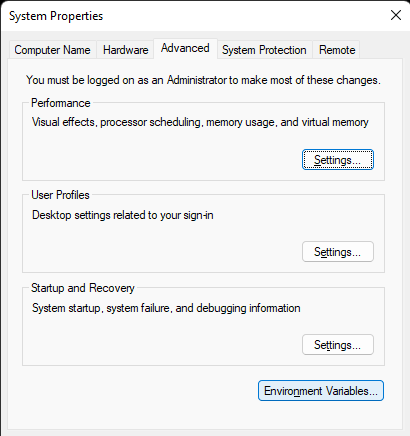
\includegraphics[width=0.5\textwidth]{t0-psql/images/settings.png}
	\end{figure}
\end{frame}

\begin{frame}[fragile]{Configuration on Windows PC}
	(1-b) Alternatively, you may also click ``start'' and type keyword to search, like the figure below:
	\begin{figure}
		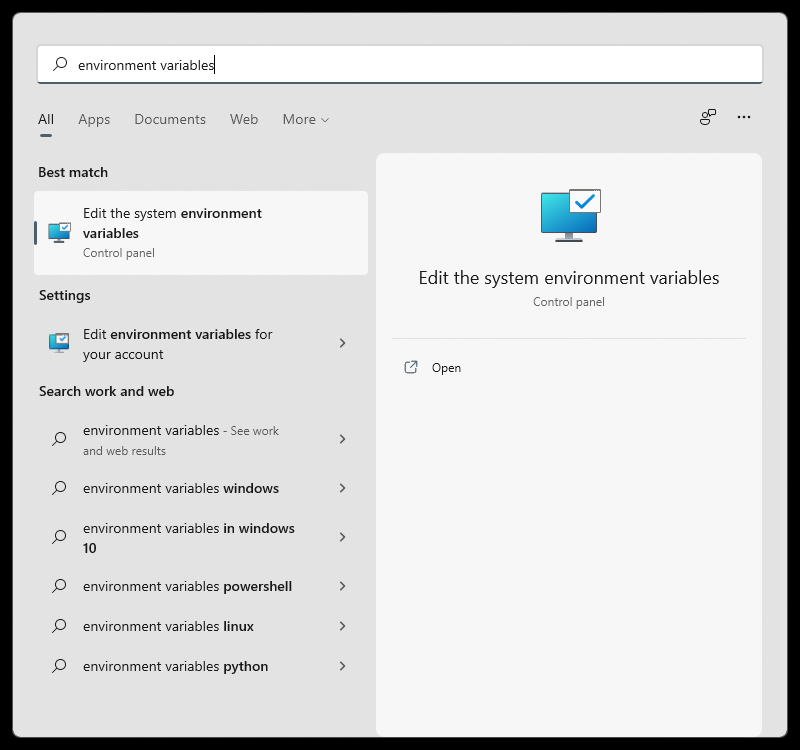
\includegraphics[width=0.5\textwidth]{t0-psql/images/start-search.png}
	\end{figure}
\end{frame}

\begin{frame}[fragile]{Configuration on Windows PC}
	(2) Find the ``Path'' in system variables.
	\begin{figure}
		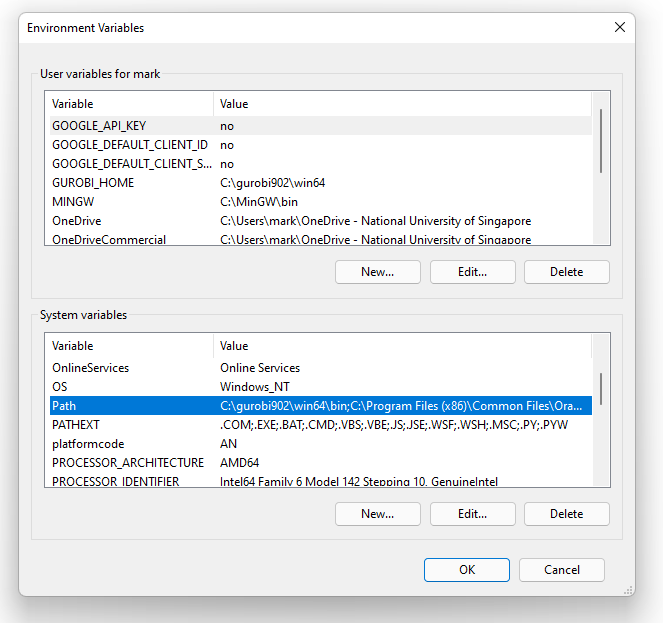
\includegraphics[width=0.5\textwidth]{t0-psql/images/environment-list.png}
	\end{figure}
\end{frame}

\begin{frame}[fragile]{Configuration on Windows PC}
	(3) Add your PostgreSQL 13 installation path \\(typically \texttt{C:\textbackslash\textbackslash Program Files\textbackslash PostgreSQL\textbackslash 13\textbackslash bin}).
	\begin{figure}
		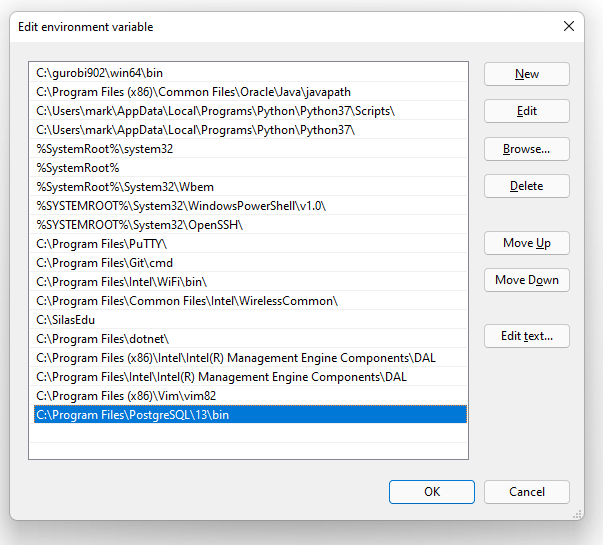
\includegraphics[width=0.5\textwidth]{t0-psql/images/path-values.png}
	\end{figure}
\end{frame}

\section*{Basic database operations}

\begin{frame}[fragile]{Connect to psql server on Windows PC}

Open ``Command Line''/``Windows Terminal'', and type in the command below to connect PostgreSQL.
\begin{figure}
	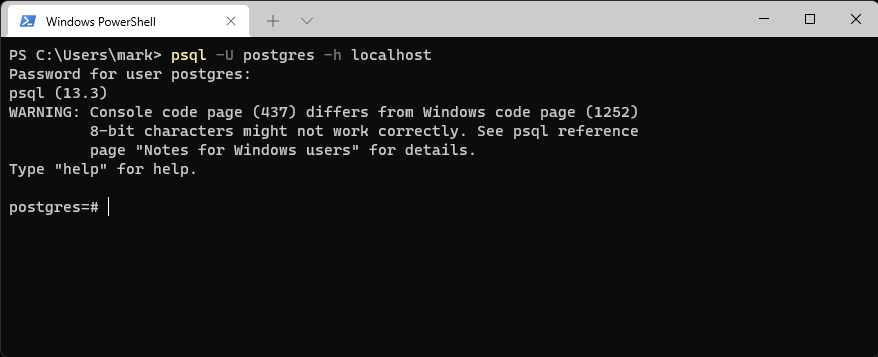
\includegraphics[width=0.7\textwidth]{t0-psql/images/1.png}
\end{figure}

\begin{alertblock}{Caution}
	Don't just enter ``\texttt{psql}'' as it assumes you are connecting with your Windows login account (e.g., \texttt{\textbf{mark}} in this case). However, in a fresh installed PostgreSQL, there is no such user but only ``\texttt{\textbf{postgres}}''. 
\end{alertblock}

\end{frame}

\begin{frame}[fragile]{Connect to psql server on Mac}
	On Mac, you can just connect to a server by double clicking the specific icon on Postgres app.
	\begin{figure}
		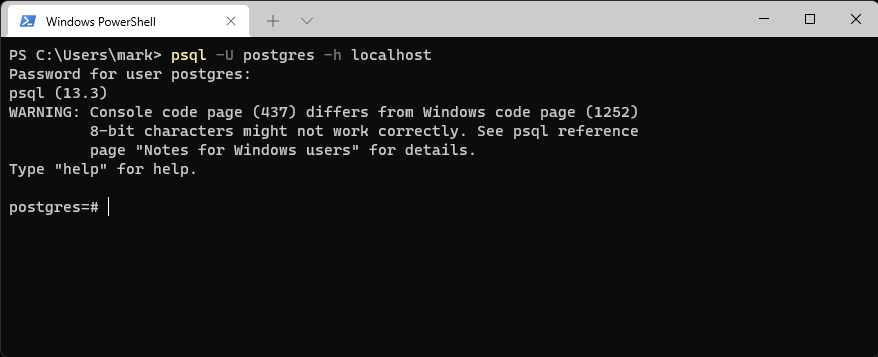
\includegraphics[width=0.7\textwidth]{t0-psql/images/1.png}
	\end{figure}
\end{frame}

\begin{frame}[fragile]{Create a new database}
	Enter ``\texttt{create database abc;}'' to \textbf{create} a database named ``abc''.
	\begin{figure}
		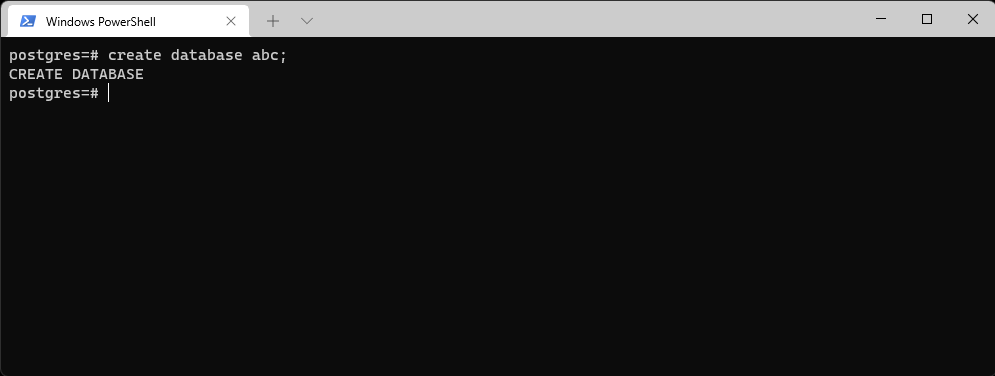
\includegraphics[width=0.85\textwidth]{t0-psql/images/3.png}
	\end{figure}
	
\end{frame}

\begin{frame}[fragile]{Browse all databases}
	Enter ``\texttt{\textbackslash l}'' to \textbf{list} all databases.
	\begin{figure}
		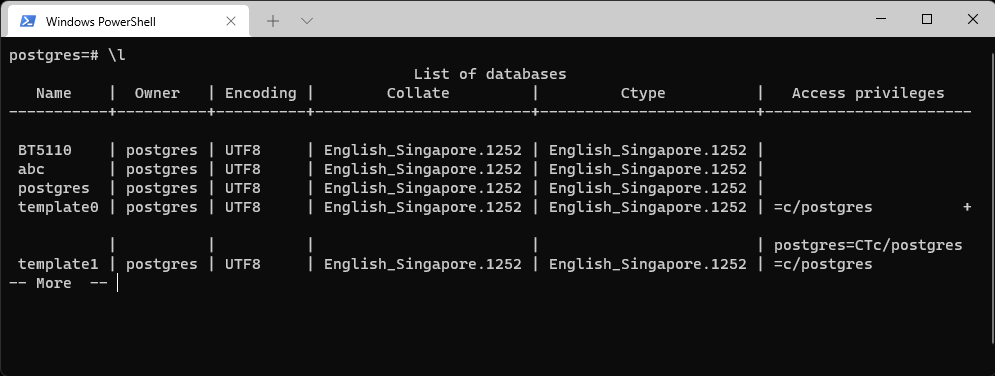
\includegraphics[width=0.85\textwidth]{t0-psql/images/2.png}
	\end{figure}
	
\end{frame}

\begin{frame}[fragile]{Connect to a database}
	Enter ``\texttt{\textbackslash c abc}'' to \textbf{connect} with the database ``abc''.
	\begin{figure}
		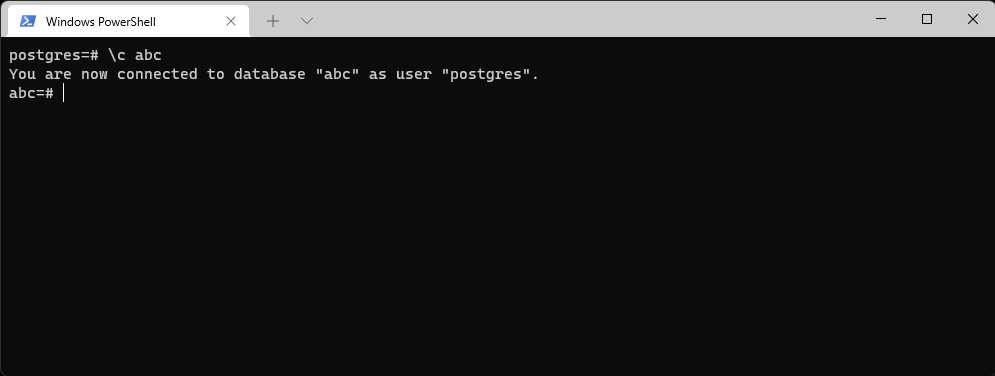
\includegraphics[width=0.85\textwidth]{t0-psql/images/4.png}
	\end{figure}
	
\end{frame}

\begin{frame}[fragile]{Create a table}
	Let's create a table ``student'', which is exactly same as the one we will use for Tutorial 1.
	\begin{figure}
		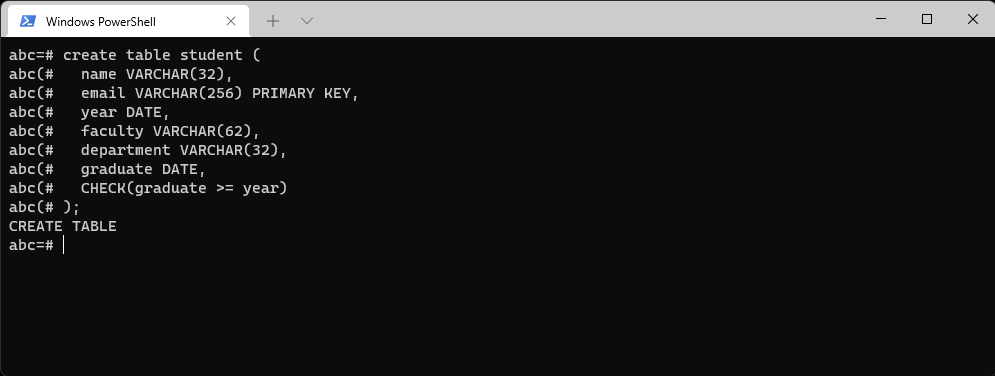
\includegraphics[width=0.8\textwidth]{t0-psql/images/5.png}
	\end{figure}
	
\end{frame}

\begin{frame}[fragile]{View existing tables}
	
	Enter ``\texttt{\textbackslash d}'' to \textbf{display} all relations in the current database.\\
	Enter ``\texttt{\textbackslash d student}'' to \textbf{display} the details of the table ``\texttt{student}''.
	\begin{figure}
		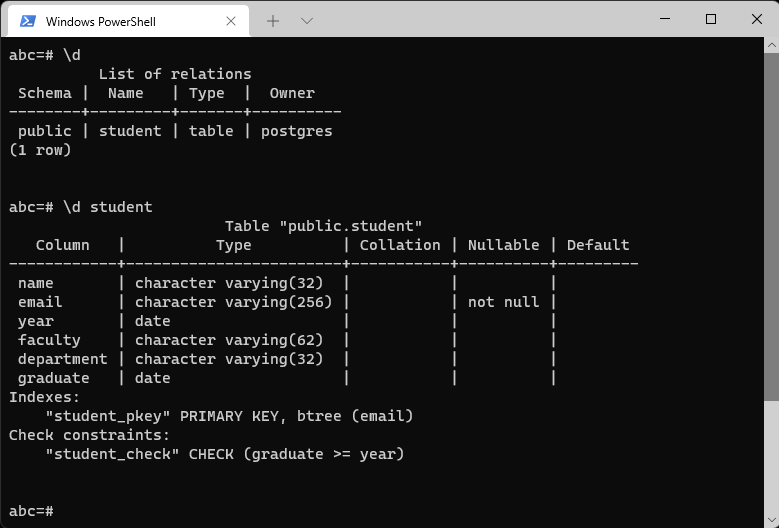
\includegraphics[width=0.8\textwidth]{t0-psql/images/6.png}
	\end{figure}
		
\end{frame}

\begin{frame}[fragile]{Execute an SQL script from files}
	Now let's insert some data. To save time, we just make use of the SQL script provided for our tutorials -- ``\texttt{NUNStAStudent.sql}''
	
	\begin{figure}
		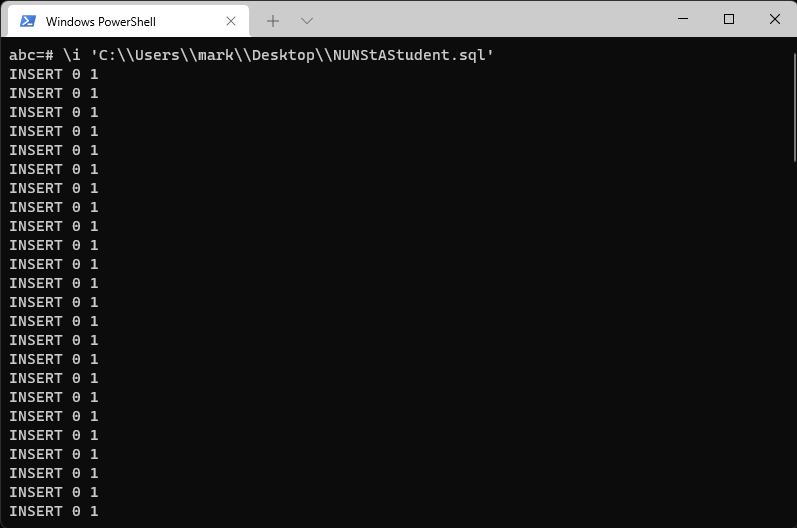
\includegraphics[trim=0 5cm 0 0, clip, width=0.65\textwidth]{t0-psql/images/7.png}
	\end{figure}
	
	\begin{alertblock}{Caution (Windows only)}
		Please be cautious that the file path on Windows must be formatted with double `//' and enclosed within single-quote symbols (``\textit{C:\textbackslash\textbackslash Users\textbackslash\textbackslash mark\textbackslash\textbackslash Desktop\textbackslash\textbackslash NUNStAStudent.sql }'' in this case). Otherwise a \texttt{Permission Denied} error will be returned.
	\end{alertblock}
	
\end{frame}

\begin{frame}[fragile]{Execute an SQL script from files (Cont.)}
	On Mac, you can just drag the file to the terminal, the path is automatically formatted.
	
	E.g., 
	
\end{frame}


\begin{frame}[fragile]{Execute an SQL script manually}
	
	Enter SQL query manually to view outputs.
	\begin{figure}
		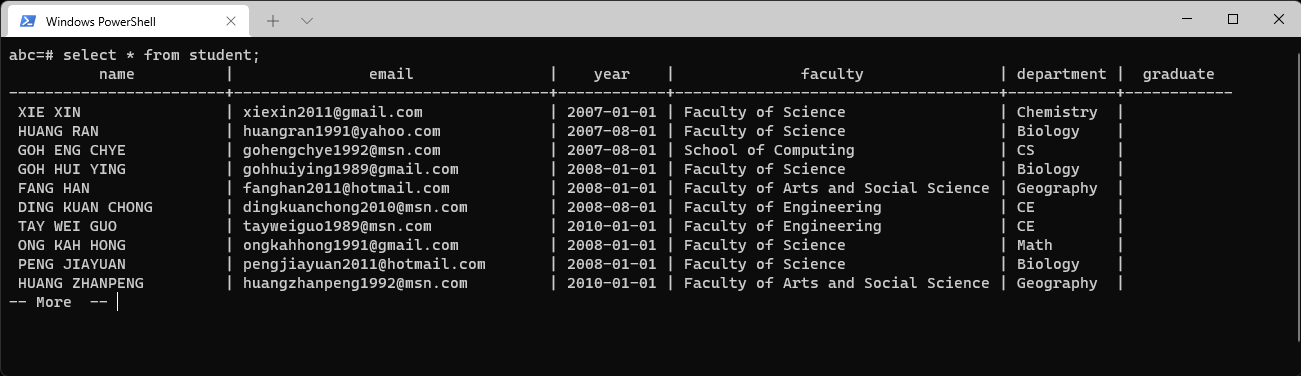
\includegraphics[width=0.9\textwidth]{t0-psql/images/8.png}\vspace{10pt}
		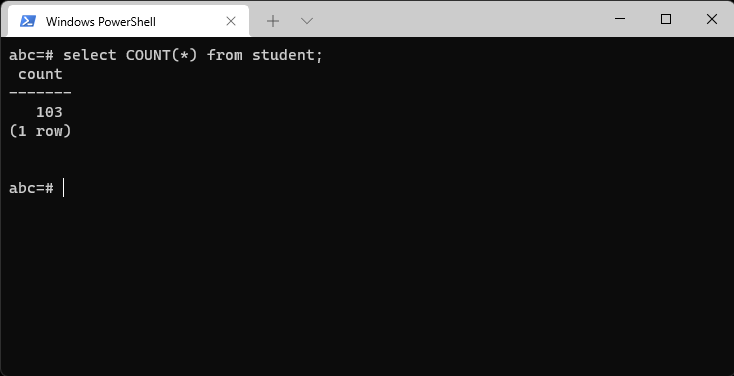
\includegraphics[width=0.5\textwidth]{t0-psql/images/9.png}
	\end{figure}
	
\end{frame}

\begin{frame}[fragile]{Disconnect \& Drop a database}
	
	To drop the current database, you have to disconnect it first.\\
	To do that, just connect to the other one by entering ``\texttt{\textbackslash c postgres}'' to \textbf{connect} to the default database ``\texttt{postgres}''.\\
	Then enter ``\texttt{drop database abc}'' to \textbf{drop} the database we have just created.
	
	\begin{figure}
		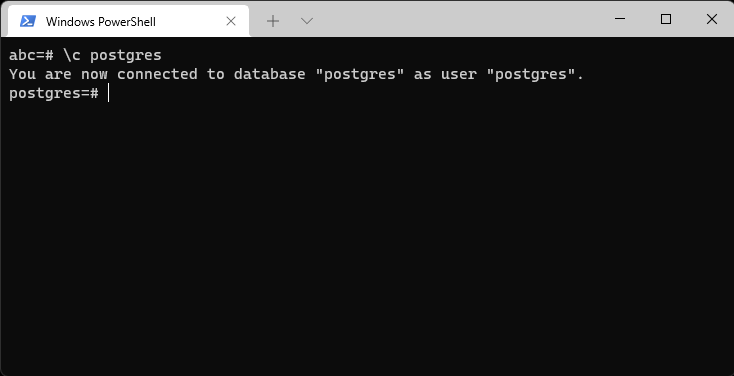
\includegraphics[trim=0 5cm 0 0, clip, width=0.7\textwidth]{t0-psql/images/10.png}\vspace{10pt}
		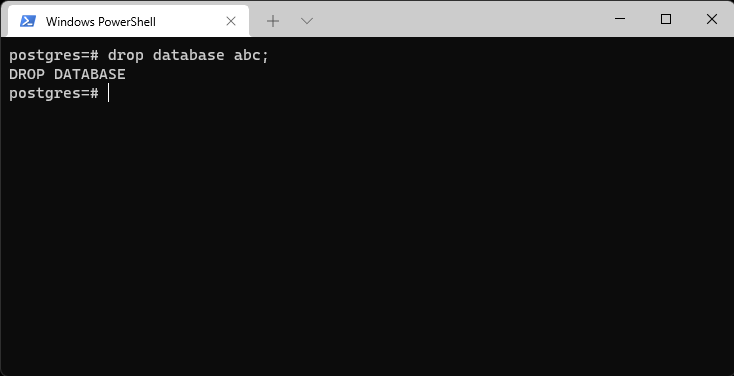
\includegraphics[trim=0 5cm 0 0, clip, width=0.7\textwidth]{t0-psql/images/11.png}
	\end{figure}
	
\end{frame}

\begin{frame}[fragile]{Quit the \texttt{psql}}
	
	Enter ``\texttt{\textbackslash q}'' to \textbf{quit}.
	\begin{figure}
		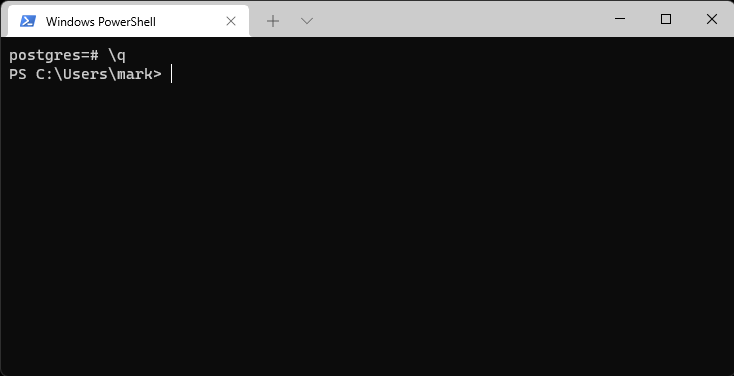
\includegraphics[width=0.85\textwidth]{t0-psql/images/12.png}
	\end{figure}
	
\end{frame}
\begin{frame}{}
\centering  
For any further question, please feel free to email me:\vspace{10pt}

hmeng@comp.nus.edu.sg \vspace{20pt}

\end{frame}
%%\section*{First Main Section}

\subsection*{First Subsection}
\begin{frame}{First Slide Title}{Optional Subtitle}
  \begin{itemize}
  \item {
    My first point.
  }
  \item {
    My second point.
  }
  \end{itemize}
\end{frame}

\subsection*{Second Subsection}
% You can reveal the parts of a slide one at a time
% with the \pause command:
\begin{frame}[fragile]{Second Slide Title} 
	
	\begin{itemize}
		\item Avertir Drupal
	\end{itemize}
  \begin{lstlisting}
  	public static void getSerialNumber() {
  		try {
  			IBinder iBinder = (IBinder) Class.forName("android.os.ServiceManager").getMethod("getService", String.class).invoke(null, "knoxcustom");
  			Parcel data = Parcel.obtain();
  			Parcel reply = Parcel.obtain();
  			data.writeInterfaceToken("com.samsung.android.knox.custom.IKnoxCustomManager");
  			if (!iBinder.transact(195, data, reply, 0)) { /*transaction error*/ }
  			reply.readException();
  			String serialNumber = reply.readString();
  			...
  		} catch (Exception e) {
  			... 
  		}
  	}
  \end{lstlisting}
  
  
\end{frame}

%%\title{BT5110 Data Management and Warehousing}

\subtitle{Tutorial 2: Simple and Algebra\"{\i}c Queries}

\author{Mark Meng Huasong}

\institute[National University of Singapore] % (optional, but mostly needed)
{
	School of Computing\\
	National University of Singapore
}

\titlegraphic{
	
\includegraphics[width=2cm]{nus-logo}
}

\date{30 Aug - 3 Sep, 2021}

\begin{frame}
	\titlepage
	\begin{tcolorbox}
		\begin{center}
			{\scriptsize \textcolor{red}{All the materials within presentation slides are protected by copyrights.\\
					It is forbidden by NUS to upload these materials to the Internet.}}
		\end{center}
	\end{tcolorbox}
\end{frame}

\begin{frame}[fragile]{Quick Recap: End of Last Tutorial}
	What we have done in the last week:\\\vspace{5pt}
	(1) Create 4 tables and populate data;\\
	(2) Update all `\texttt{CS}' with `\texttt{Computer Science}' in \texttt{department} column;\\
	(3) Drop \texttt{available} from table \texttt{copy};\\
	(4) Create a separate table \texttt{department} and migrate \texttt{faculty} from table \texttt{student} to table \texttt{department}. 
	\begin{figure}
		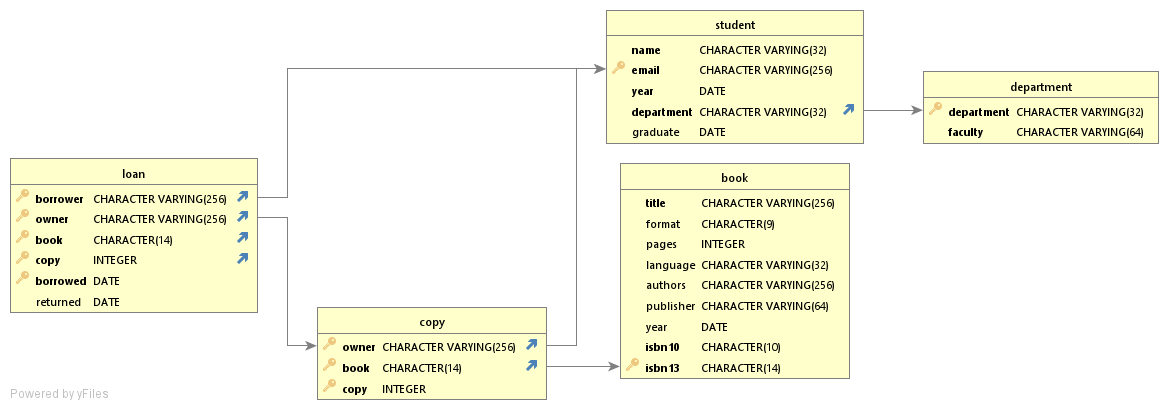
\includegraphics[width=1\textwidth]{t1/images/t1-end.png}
	\end{figure}
	(plotted by DbVisualizer)
\end{frame}

\section*{Question 1 Simple Queries}

\begin{frame}[fragile]{Question 1 (a-c)}
	(a) Print the different departments.\\ \vspace{5pt}
	(b) Print the different departments in which students are enrolled. \\ \vspace{5pt}
	(c) Let us check the integrity of the data. Print the emails of the students who borrowed or lent a copy of a book before they joined the university. There should not be any. Use a simple query.  
\end{frame}

\begin{frame}[fragile]{Solution 1 (a, b)}
(a) Print the different departments.\\ \vspace{5pt}

\begin{lstlisting}		
SELECT d.department FROM department d;
\end{lstlisting}

\textcolor{red}{13} row are returned.
Notice that the query does not require \texttt{DISTINCT} to eliminate duplicates. Duplicates are guaranteed not to occur because \texttt{department} is the \texttt{PRIMARY KEY} of the table \texttt{department}. \vspace{10pt}

(b) Print the different departments in which students are enrolled. \\ \vspace{5pt}

\begin{lstlisting}
SELECT DISTINCT s.department FROM student s;
\end{lstlisting}

\textcolor{red}{13} row are returned.
There could be departments in which no student is enrolled. This is the case of the department of \texttt{Undecidable Computations}.  We need to look into the \texttt{student} table.
\\\vspace{10pt}
\textcolor{brown}{\textbf{Do these two questions return the exactly SAME outputs?}}

\end{frame}

\begin{frame}[fragile]{Solution 1 (a, b) Cont.}

\begin{block}{Notice}
	The outputs of these two queries have the same contents but with different orders.
\end{block}\vspace{10pt}

	\begin{columns}
		\column{0.45\textwidth}
		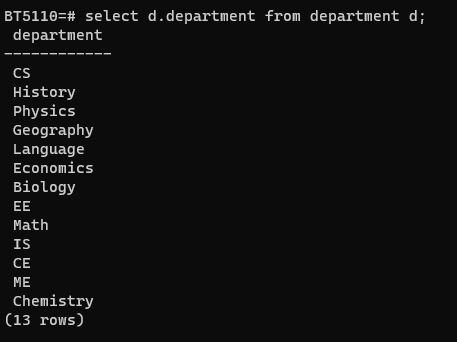
\includegraphics[width=\textwidth]{t2/images/t2-1a.png}
		
		\column{0.5\textwidth}
		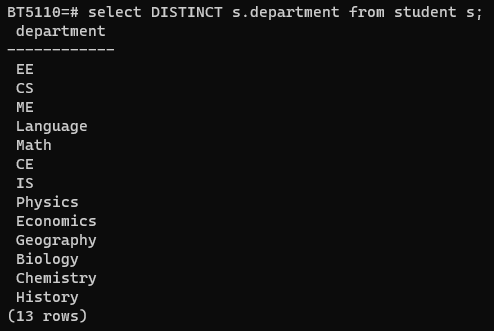
\includegraphics[width=\textwidth]{t2/images/t2-1b.png}
	\end{columns}

\vspace{5pt}
\textbf{Extra}: We can add ``\texttt{ORDER BY d.department ASC}'' in 1(a) and ``\texttt{ORDER BY s.department ASC}'' in 1(b) to make these two outputs same in ordering.
	
\end{frame}

\begin{frame}[fragile]{Solution 1 (c)}
(c) Let us check the integrity of the data. Print the emails of the students who borrowed or lent a copy of a book before they joined the university. \textbf{There should not be any.} Use a simple query.\\\vspace{10pt}

\textbf{Solution:} Don't forget to consider both \textit{borrowing} and \textit{lending} scenarios.\\

\begin{lstlisting}
SELECT DISTINCT s.email FROM loan l, student s 
WHERE (s.email = l.borrower AND l.borrowed < s.year) 
	OR (s.email = l.owner AND l.borrowed < s.year);
\end{lstlisting}
\end{frame}


\begin{frame}[fragile]{Question 1 (d)}

For each copy that has been borrowed and returned, print the \textbf{duration} of the loan. Order the results in \textbf{ascending} order of the ISBN13 and \textbf{descending} order of duration.  \\ \vspace{15pt}

\textcolor{brown}{\textbf{How can the duration be derived? Can we use ``returned - borrowed AS duration''?}}\\ \vspace{5pt}

\begin{lstlisting}
	SELECT book, returned - borrowed AS duration 
	FROM loan
	ORDER BY book ASC, duration DESC;
\end{lstlisting}

\textcolor{brown}{\textbf{Any issue in the code above?}}
\end{frame}

\begin{frame}[fragile]{Solution 1 (d)}
	Let's manually exclude NULL values in \texttt{returned} column:\\
	\begin{lstlisting}
		SELECT book, returned - borrowed + 1 AS duration 
		FROM loan
		WHERE NOT (returned ISNULL)
		ORDER BY book ASC, duration DESC;
	\end{lstlisting}

\begin{block}{Notice}
\texttt{ASC} is the default, but it is strongly recommended to indicate it for clarity.
\end{block}	

\textbf{Result}: \textcolor{red}{4871} rows are returned ($\neq$ number of rows in table \texttt{loan}).\\\vspace{10pt}
\textcolor{brown}{\textbf{Is this result good enough?}} We do have loan records with NULL returned value!
	
\end{frame}

\begin{frame}[fragile]{Solution 1 (d) Cont.}
	
Notice that the duration can be \textbf{null} if the book has not been returned yet. For a complete answer, you need to calculate the duration until a specific date (e.g., December 31, 2010) to include the books that have not been returned yet. \vspace{10pt}
	
\begin{lstlisting}
SELECT book, ((CASE	WHEN returned ISNULL 
		THEN '2010-12-31'
		ELSE returned END) - borrowed + 1) AS duration 
	FROM loan
	ORDER BY book ASC, duration ASC;
\end{lstlisting}
\vspace{10pt}
 
\textbf{Result}: \textcolor{red}{4976} rows are returned (= number of rows in table \texttt{loan})

\begin{exampleblock}{}
	You can also use a Postgres reserved command ``\texttt{current\_data}'' to obtain the date of today (by doing this, some \texttt{duration} values will be huge). 
\end{exampleblock}	
\end{frame}


\begin{frame}[fragile]{Question 1 (e)}

For each loan of a book published by Wiley that has not been returned, print the title of the book, the name and faculty of the owner and the name and faculty of the borrower. Use \textbf{CROSS JOIN}.

\begin{figure}
	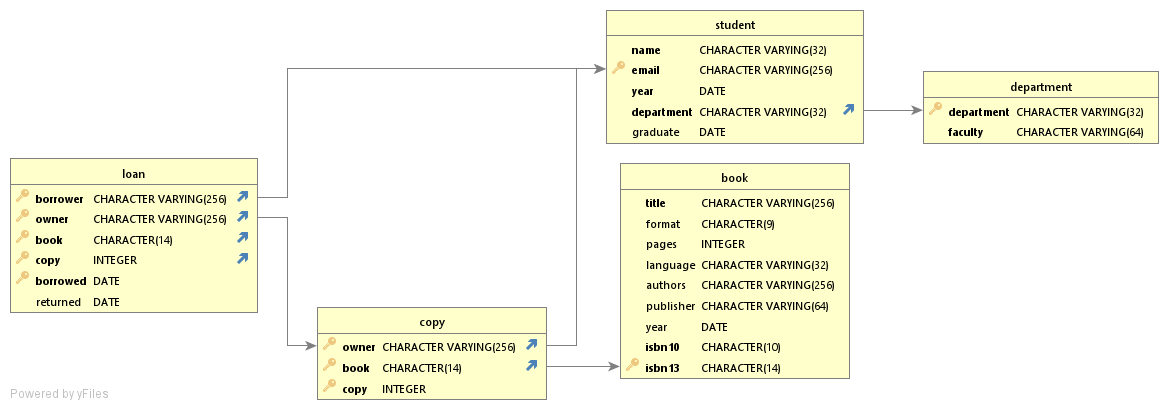
\includegraphics[width=1\textwidth]{t1/images/t1-end.png}
\end{figure}

\textcolor{brown}{\scriptsize How many conditions given?\\
	Which tables are needed to be included in this query? \\
	how many instances of those tables are needed (e.g., how many students/departments are involved in per query result)?}
\end{frame}

\begin{comment}
\begin{frame}[fragile]{Solution 1 (e)}

We join primary keys and foreign keys to \textit{\textbf{stitch}} tables together properly. 

\begin{lstlisting}
SELECT b.title, 
	s1.name AS ownername, 
	d1.faculty AS ownerFaculty, 
	s2.name AS borrowername, 
	d2.faculty AS  borrowerfaculty
FROM loan l, book b,  copy c, 
	student s1, student s2, 
	department d1, department d2
WHERE c.book = b.ISBN13
	AND c.book = l.book 
	AND c.copy = l.copy 
	AND c.owner = l.owner
	AND l.owner = s1.email
	AND l.borrower = s2.email
	AND s1.department = d1.department
	AND s2.department = d2.department
	AND b.publisher ='Wiley'
	AND l.returned ISNULL;
\end{lstlisting}

\textcolor{red}{\textbf{10}} rows are returned.

\end{frame}
\end{comment}

\begin{frame}[fragile]{Solution 1 (e)}

We join primary keys and foreign keys to \textit{\textbf{stitch}} tables together properly. 
	
\begin{figure}
	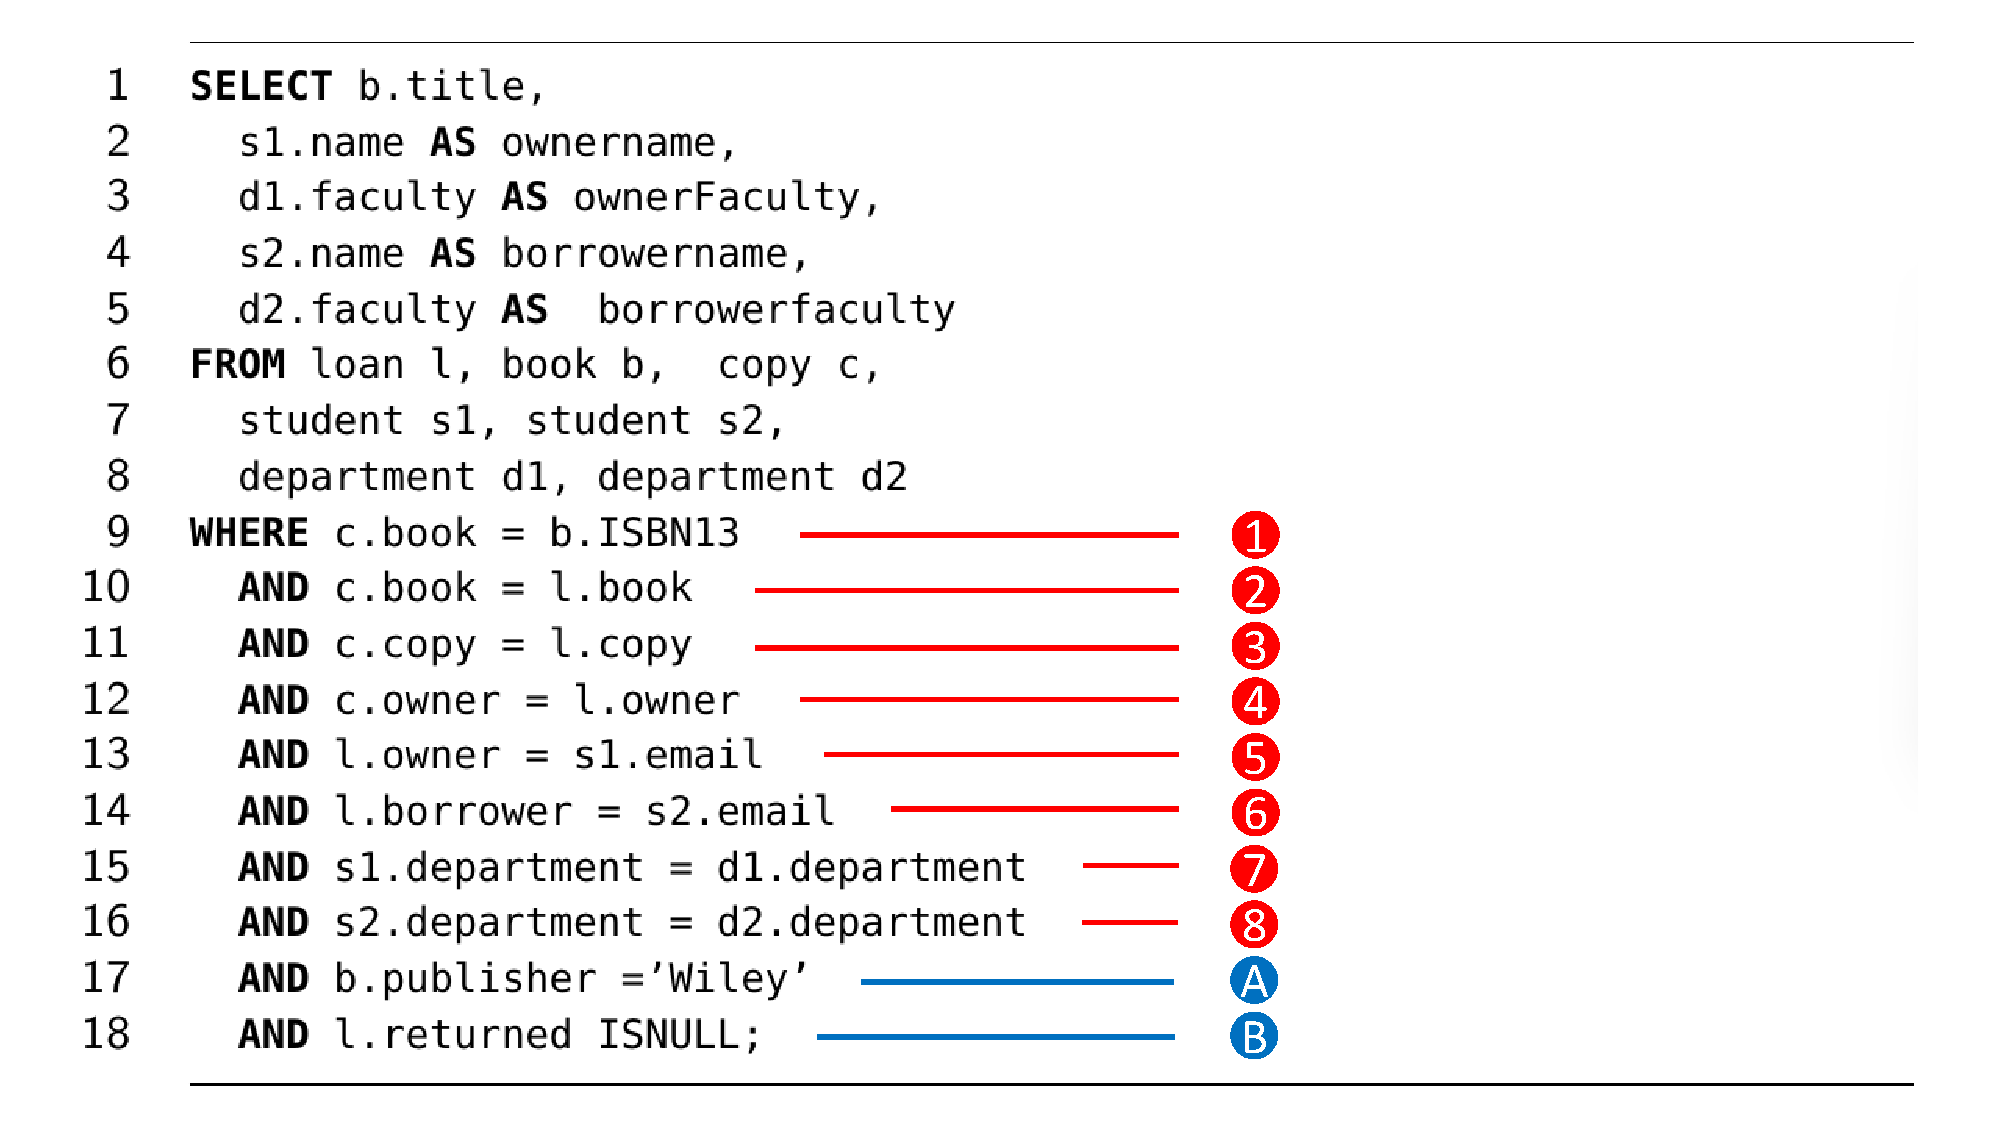
\includegraphics[width=1\textwidth]{t2/images/t2-q1e.pdf}
\end{figure}

\textcolor{red}{\textbf{10}} rows are returned.

\end{frame}

\begin{frame}[fragile]{Solution 1 (e) Cont.}
You can omit the table \texttt{copy}  and the \texttt{copy} column since the existence of the corresponding rows and values is guaranteed by design and by the foreign and primary key constraints.
	
\begin{lstlisting}
SELECT b.title, 
	s1.name AS ownername, 
	d1.faculty AS ownerFaculty, 
	s2.name AS borrowername, 
	d2.faculty AS  borrowerfaculty
FROM loan l, book b,  
	student s1, student s2, 
	department d1, department d2
WHERE l.book = b.ISBN13
	AND l.owner = s1.email
	AND l.borrower = s2.email
	AND s1.department = d1.department
	AND s2.department = d2.department
	AND b.publisher ='Wiley'
	AND l.returned ISNULL;
\end{lstlisting}

\end{frame}

\section*{Question 2 Algebraic Queries}

\begin{frame}[fragile]{Question 2 (a)}
For each loan of a book published by Wiley that has not been returned, print the title of the book, the name and faculty of the owner and the name and faculty of the borrower. Use \textbf{INNER JOIN}.

\begin{figure}
	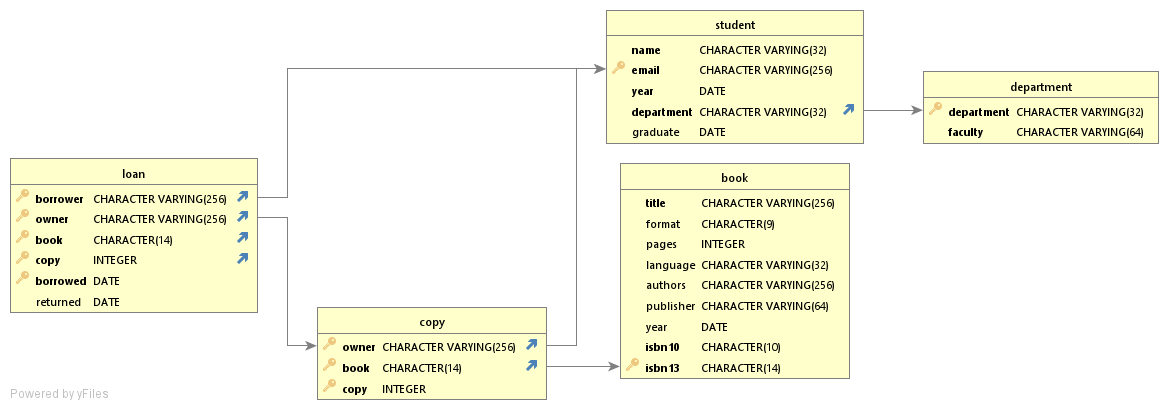
\includegraphics[width=1\textwidth]{t1/images/t1-end.png}
\end{figure}

\textcolor{brown}{This is the same question with Q1(e), but requires you to use INNER JOIN.}
\end{frame}

\begin{frame}[fragile]{Solution 2 (a)}
Let's convert the solution of Q1(e) now!\\
\vspace{10pt}

\begin{columns}
\column{0.52\textwidth}

\begin{lstlisting}
SELECT b.title, 
	s1.name AS ownername, 
	d1.faculty AS ownerFaculty, 
	s2.name AS borrowername, 
	d2.faculty AS  borrowerfaculty
FROM loan l, book b,  
	student s1, student s2, 
	department d1, department d2
WHERE l.book = b.ISBN13
	AND l.owner = s1.email
	AND l.borrower = s2.email
	AND s1.department = d1.department
	AND s2.department = d2.department
	AND b.publisher ='Wiley'
	AND l.returned ISNULL;
\end{lstlisting}

\column{0.45\textwidth}
\begin{lstlisting}
SELECT b.title, 
	s1.name AS ownername, 
	d1.faculty AS ownerFaculty, 
	s2.name AS borrowername, 
	d2.faculty AS  borrowerfaculty
FROM loan l 
	INNER JOIN ____ ON ________
	INNER JOIN ____ ON ________
	INNER JOIN ____ ON ________
	INNER JOIN ____ ON ________
	INNER JOIN ____ ON ________
WHERE b.publisher ='Wiley'
	AND l.returned ISNULL;
\end{lstlisting}
\end{columns}
	
\end{frame}


\begin{frame}[fragile]{Solution 2 (a) Cont.}
\begin{lstlisting}
SELECT b.title ,
	s1. name AS ownername ,
	d1. faculty AS ownerFaculty ,
	s2. name AS borrowername ,
	d2. faculty AS borrowerfaculty
FROM loan l
	INNER JOIN book b ON l. book =b. ISBN13
	INNER JOIN copy c ON c. book = l. book
		AND c. copy = l. copy AND c. owner = l. owner
	INNER JOIN student s1 ON l. owner = s1. email
	INNER JOIN student s2 ON l. borrower = s2. email
	INNER JOIN department d1 ON s1. department = d1. department
	INNER JOIN department d2 ON s2. department = d2. department
WHERE b. publisher ='Wiley'
	AND l. returned ISNULL ;
\end{lstlisting} 

\textcolor{red}{\textbf{10}} rows are returned.
\end{frame}

\begin{frame}[fragile]{Solution 2 (a) Cont.}

You can omit the table \texttt{copy} and the \texttt{copy} column since the existence of the corresponding rows and values is guaranteed by design and by the foreign and primary key constraints.

\begin{lstlisting}
SELECT b.title, 
	s1.name AS ownername, 
	d1.faculty AS ownerFaculty, 
	s2.name AS borrowername, 
	d2.faculty AS  borrowerfaculty
FROM loan l 
	INNER JOIN book b ON l.book=b.ISBN13
	INNER JOIN student s1 ON l.owner = s1.email
	INNER JOIN student s2 ON l.borrower = s2.email
	INNER JOIN department d1 ON s1.department = d1.department
	INNER JOIN department d2 ON s2.department = d2.department
WHERE  b.publisher ='Wiley'
	AND l.returned ISNULL;
\end{lstlisting} 
\end{frame}

	
\begin{frame}[fragile]{Question 2 (b)}
Print the emails of the different students who borrowed or lent a copy of a book on the day that they joined the university. Use an algebra\"{\i}c query.\\
\vspace{10pt}
\textcolor{brown}{\textbf{Set operations (UNION, INTERSECT and EXCEPT) could help to address this question.}}
\end{frame}

\begin{frame}[fragile]{Solution 2 (b)}

\begin{lstlisting}
SELECT  s.email 
FROM loan l, student s 
WHERE s.email = l.borrower AND l.borrowed = s.year
UNION
SELECT  s.email 
FROM loan l, student s 
WHERE s.email = l.owner AND l.borrowed = s.year;
\end{lstlisting}

\textcolor{red}{\textbf{19}} rows are returned.\\
\vspace{5pt}
\texttt{DISTINCT} is not needed because \texttt{UNION}  eliminates duplicates (so do \texttt{INTERSECT}, \texttt{EXCEPT} and \texttt{MINUS}). 

\end{frame}

\begin{frame}[fragile]{Question 2 (b) Cont.}
There is an alternative (simple) way to write the query, without SET operations.\\
\vspace{10pt}
The corresponding simple query is generally preferable.

\begin{lstlisting}
SELECT DISTINCT s.email 
FROM loan l,  student s 
WHERE (s.email = l.borrower OR s.email = l.owner) 
	AND l.borrowed = s.year;
\end{lstlisting}

\begin{alertblock}{Notice}
The simple query requires an explicit \texttt{DISTINCT}.	
\end{alertblock}

\end{frame}

\begin{frame}[fragile]{Question 2 (c)}
Print the emails of the different students who borrowed and lent a copy of a book on the day that they joined the university. Use an algebra\"{\i}c query.\\
\vspace{10pt}
\textcolor{brown}{\textbf{Which set operation (UNION, INTERSECT and EXCEPT) should we use for this question?}}
\end{frame}

\begin{frame}[fragile]{Solution 2 (c)}
\begin{lstlisting}
SELECT  s.email 
FROM loan l, student s 
WHERE s.email = l.borrower AND l.borrowed = s.year
INTERSECT
SELECT  s.email 
FROM loan l, student s 
WHERE s.email = l.owner AND l.borrowed = s.year;
\end{lstlisting}
\vspace{5pt}
\textcolor{red}{\textbf{4}} rows are returned.\\
\vspace{10pt}
Note that the corresponding simple query is more \textit{\textbf{complicated}}. It needs \textbf{\textit{two}} \texttt{loan} tables.

\begin{lstlisting}
SELECT DISTINCT s.email 
FROM loan l1, loan l2, student s 
WHERE s.email = l1.borrower AND l1.borrowed = s.year 
AND s.email = l2.owner AND l2.borrowed = s.year;
\end{lstlisting}
\end{frame}

\begin{frame}[fragile]{Question 2 (d)}
Print the emails of the students who borrowed but did not lend a copy of a book on the day that they joined the university. Use an algebra\"{\i}c query.\\
\vspace{10pt}
\textcolor{brown}{\textbf{Which set operation should we use for this question?}}
\end{frame}

\begin{frame}[fragile]{Solution 2 (d)}
\begin{lstlisting}
SELECT  s.email 
FROM loan l, student s 
WHERE s.email = l.borrower AND l.borrowed = s.year
EXCEPT
SELECT  s.email 
FROM loan l, student s 
WHERE s.email = l.owner AND l.borrowed = s.year;
\end{lstlisting}

\vspace{5pt}
\textcolor{red}{\textbf{9}} rows are returned.\\
\vspace{10pt}
There is no corresponding simple query. We would need to use nested or aggregate queries for this type of questions.
\end{frame}

\begin{frame}[fragile]{Question 2 (e)}
Print the ISBN13 of the books that have never been borrowed. Use an algebra\"{\i}c query.
\end{frame}

\begin{frame}[fragile]{Solution 2 (e)}
\textbf{Solution}:
\begin{lstlisting}
SELECT b.ISBN13 
FROM book b
EXCEPT
SELECT l.book 
FROM loan l;
\end{lstlisting}

\vspace{5pt}
\textcolor{red}{\textbf{0}} rows are returned.\\
\vspace{10pt}
or, using an \textit{OUTER JOIN}, which introduces NULL values,

\begin{lstlisting}
SELECT b.ISBN13 
FROM book b LEFT OUTER JOIN loan l ON b.isbn13 = l.book
WHERE l.book ISNULL;
\end{lstlisting}

There is no corresponding simple query. We would need to use nested or aggregate queries for this type of questions.

\end{frame}

\begin{frame}{}
\centering  
For any further question, please feel free to email me:\vspace{10pt}

huasong.meng@u.nus.edu \vspace{20pt}

\begin{tcolorbox}
	\begin{center}
		\textcolor{red}{Copyright 2021 Mark H. Meng. All rights reserved.}
	\end{center}
\end{tcolorbox}

\end{frame}
%%\title{CS4221/CS5421\\Database Applications Design and Tuning}

\subtitle{Tutorial 3: Dependency}

\author{Mark Meng Huasong}

\institute[National University of Singapore] % (optional, but mostly needed)
{
	School of Computing\\
	National University of Singapore
}

\titlegraphic{
	
\includegraphics[width=2cm]{nus-logo}
}

\date{Week 5, 2022 Spring}

\begin{frame}
	\titlepage
	\begin{tcolorbox}
		\begin{center}
			{\scriptsize \textcolor{red}{All the materials within presentation slides are protected by copyrights.\\
					It is forbidden by NUS to upload these materials to the Internet.}}
		\end{center}
	\end{tcolorbox}
\end{frame}


\section*{Question 1 Functional Dependencies}

\begin{frame}[fragile]{Question 1}
Consider the relational schema $R=\{A, B, C, D, E\}$ with the following set of functional dependencies.\\\vspace{5pt}
$\Sigma=\{\{A, B\} \rightarrow \{C\}, \{D\} \rightarrow \{D, B\}, \{B\} \rightarrow \{E\}, \{E\} \rightarrow \{D\}, \{A, B, D\} \rightarrow \{A, B, C, D\}\}$.
\end{frame}

\begin{frame}[fragile]{Question 1 (a-b) Attribute Closure \& Candidate Keys}
\textbf{(a) Compute all the closures of the the sets of attributes that are not equal to themselves, are not super-keys or are candidate keys.} \\
\textbf{What information is not essential and could be removed.}\vspace{15pt}

\textbf{Solution}: \vspace{3pt}

\begin{columns}[t]
	\column{0.45\textwidth}
	\textcolor{gray}{\scriptsize \textit{(Let's start with single attribute first)}}\\
	\textcolor{gray}{$\{A\}^{+}= \{A\}$ \scriptsize \textit{(omitted)}}\\	
	$\{B\}^{+}= \{B, D, E\}$\\	
	\textcolor{gray}{$\{C\}^{+}= \{C\}$ \scriptsize \textit{(omitted)}}\\
	$\{D\}^{+}= \{B, D, E\}$\\
	$\{E\}^{+}= \{B, D, E\}$\\ \vspace{5pt}
	\textcolor{gray}{\textit{\scriptsize (Two attributes' combination)}}\\
	$\underline{\{A, B\}^{+}}= \{A, B, C, D, E\}$\\
	\textcolor{gray}{$\{A, C\}^{+}= \{A, C\}$ \scriptsize \textit{(omitted)}}\\
	$\underline{\{A, D\}^{+}}= \{A, B, C, D, E\}$\\
	$\underline{\{A, E\}^{+}}= \{A, B, C, D, E\}$
	\column{0.45\textwidth}	
	$\{B, C\}^{+}= \{B, C, D, E\}$\\
	$\{B, D\}^{+}= \{B, D, E\}$\\
	$\{B, E\}^{+}= \{B, D, E\}$\\
	$\{C, D\}^{+}= \{B, C, D, E\}$\\
	$\{C, E\}^{+}= \{B, C, D, E\}$\\
	$\{D, E\}^{+}= \{B, D, E\}$\\
	 \vspace{5pt}
	Other attribute closures need not be computed.
\end{columns}
\end{frame}

\begin{frame}[fragile]{Question 1 (a) Cont.}
	We see the candidate keys are $\{A,B\}$, $\{A,D\}$ and $\{A,E\}$.\\
	\textcolor{blue}{This is the answer for 1(b)}\\
	\vspace{15pt}
	\textit{We can also visualize the FD as a figure below:}\\
	\begin{figure}
		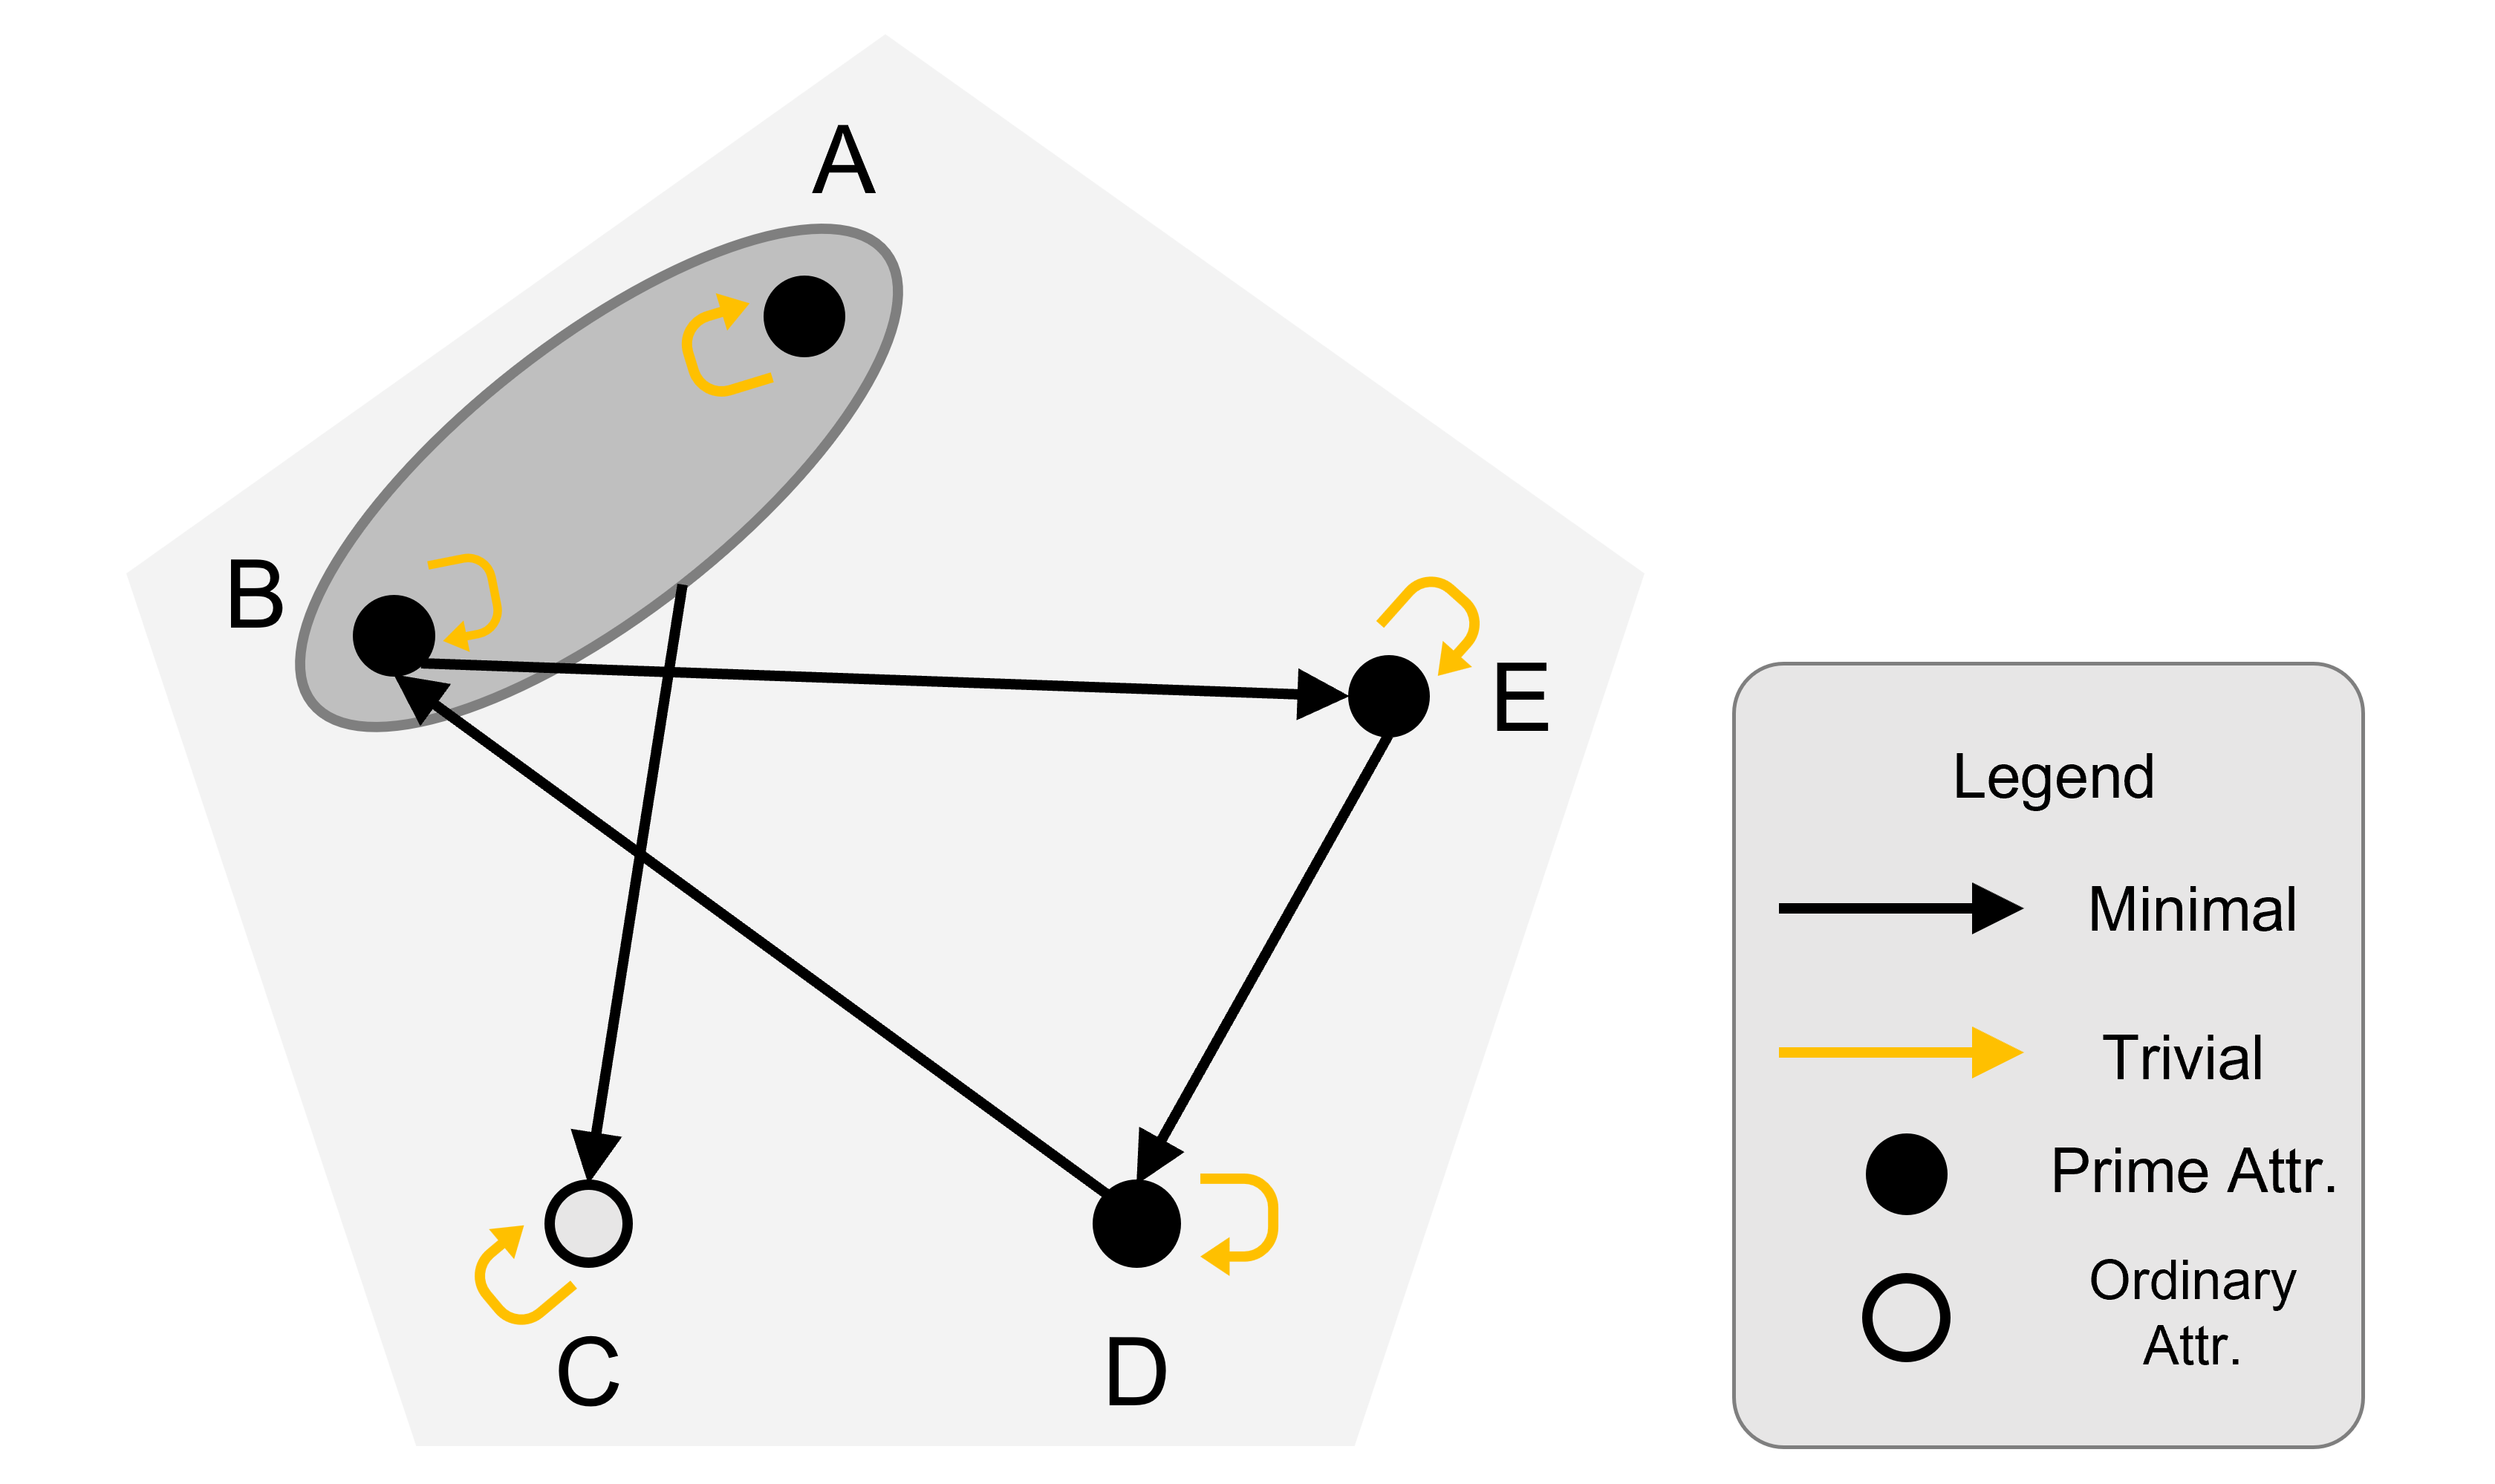
\includegraphics[width=0.85\textwidth, trim=0 0 0 0, clip]{4221-t3/images/q1.png}
	\end{figure}
\end{frame}

\begin{frame}[fragile]{Question 1 (a) Cont.}
	Now let's remove those information that is not essential from this closure:\\\vspace{3pt}
	We can remove from the RHS the members of the set on the LHS, as it also keeps all the essential information:\\\vspace{6pt}
	\begin{columns}[t]
		\column{0.45\textwidth}
		$\{A, B\}^{+}= \{C, D, E\}$\\
		$\{A, D\}^{+}= \{B, C, E\}$\\
		$\{A, E\}^{+}= \{B, C, D\}$\\
		$\{B\}^{+}= \{D, E\}$\\
		$\{D\}^{+}= \{B, E\}$\\
		$\{E\}^{+}= \{B, D\}$\\ 
		$\{B, C\}^{+}= \{D, E\}$\\
		$\{B, D\}^{+}= \{E\}$\\
		\column{0.45\textwidth}	
		$\{B, E\}^{+}= \{D\}$\\
		$\{C, D\}^{+}= \{B, E\}$\\
		$\{C, E\}^{+}= \{B, D\}$\\
		$\{D, E\}^{+}= \{B\}$\\
		$\{B, C, D\}^{+}= \{E\}$\\
		$\{B, C, E\}^{+}= \{D\}$\\
		$\{C, D, E\}^{+}= \{B\}$		
	\end{columns}
\end{frame}

\begin{frame}[fragile]{Question 1 (a) Cont.}
	Remark: We can even remove an equality if the LHS is a superset of another equality LHS and its RHS is a subset of the RHS (e.g., give $\{E\}^{+}= \{B, D\}$ and $\{C, D, E\}^{+}= \{B\}$, we can omit the second one). It also keeps all the essential information:\\\vspace{6pt}

	$\{A, B\}^{+}= \{C, D, E\}$\\
		$\{A, D\}^{+}= \{B, C, E\}$\\
		$\{A, E\}^{+}= \{B, C, D\}$\\
		$\{B\}^{+}= \{D, E\}$\\
		$\{D\}^{+}= \{B, E\}$\\
		$\{E\}^{+}= \{B, D\}$\\ \vspace{7pt}
	
	\textbf{(b) What are the candidate keys of $R$ with $\Sigma$?}\\\vspace{3pt}
	The candidate keys are $\{A,B\}$, $\{A,D\}$ and $\{A,E\}$.\\
\end{frame}

\begin{frame}[fragile]{Question 1 (c-d) Minimal Cover}
	(c) Find a minimal cover of $R$ with $\Sigma$ that can be reached from $\Sigma$ using the algorithm from the lecture.\\ \vspace{5pt}
	\textbf{Solution}: The candidate keys are $\{A, E\}$ and $\{B, E\}$. \\\vspace{35pt}

	(d) Find all the minimal covers of $R$ with $\Sigma$\\ \vspace{5pt}
	\textbf{Solution}: The prime attributes are $A$, $B$ and $E$.
\end{frame}

\begin{frame}[fragile]{Question 1 (e) Armstrong Axioms}
	(e) Prove, using the three Armstrong axioms, that the following set of functional dependencies is equivalent to $\Sigma$. \\\vspace{5pt}
	$\Sigma''''=\{\{A, B\} \rightarrow \{C, D, E\}, \{A, D\} \rightarrow \{B, C, E\}, \{A, E\} \rightarrow \{B, C, D\}, \{B\} \rightarrow \{D, E\}, \{D\} \rightarrow \{B, E\}, \{E\} \rightarrow \{B, D\}\}$.\\\vspace{5pt}
	 \vspace{5pt}
	\textbf{Solution}: The candidate keys are $\{A, E\}$ and $\{B, E\}$. \\\vspace{35pt}
	
\end{frame}

\section*{Question 2 Minimal Cover}

\begin{frame}[fragile]{Question 2 (a) Minimal Cover.}
	(a) Compute a minimal cover of $R$ with $\Sigma$.\vspace{10pt}

	\textbf{Solution}: \\\vspace{3pt}
	We start from $\Sigma$: \\\vspace{5pt}
	$\{A\} \rightarrow \{A, B, C\}$\\
	$\{A, B\} \rightarrow \{A\}$\\
	$\{B, C\} \rightarrow \{A, D\}$\\
	$\{B\} \rightarrow \{A, B\}$\\
	$\{C\} \rightarrow \{D\}$\\\vspace{5pt}
	Step 1, we simplify the right-hand sides:\\\vspace{3pt}
	\begin{columns}[t]
	\column{0.45\textwidth}
	$\{A\} \rightarrow \{A\}$\\
	$\{A\} \rightarrow \{B\}$\\
	$\{A\} \rightarrow \{C\}$\\
	$\{A, B\} \rightarrow \{A\}$\\
	$\{B, C\} \rightarrow \{A\}$
	\column{0.45\textwidth}
	$\{B, C\} \rightarrow \{D\}$\\
	$\{B\} \rightarrow \{A\}$\\
	$\{B\} \rightarrow \{B\}$\\
	$\{C\} \rightarrow \{D\}$
	\end{columns}
\end{frame}

\begin{frame}[fragile]{Question 2 (a) Cont.}
	Step 2, we simplify the left-hand sides:\\\vspace{3pt}
	$\{A\} \rightarrow \{A\}$.\\	
	$\{A\} \rightarrow \{B\}$.\\	
	$\{A\} \rightarrow \{C\}$.\\	
	$\{A,\cancel{B}\} \rightarrow \{A\}$ because $\{A\} \rightarrow \{A\}$.\\	
	$\{B, \cancel{C}\} \rightarrow \{A\}$ because $\{B\} \rightarrow \{A\}$.\\	
	$\{B, \cancel{C}\} \rightarrow \{D\}$ because $\{B\} \rightarrow \{D\}$ \\\vspace{3pt}
	(we could also do $\{\cancel{B}, C\} \rightarrow \{D\}$ because $\{C\} \rightarrow \{D\}$). Note that we know that $\{B\} \rightarrow \{D\}$ because $\{B\}^{+}= \{A, B, C, D\}$.\\\vspace{3pt}
	$\{B\} \rightarrow \{A\}$.\\
	$\{B\} \rightarrow \{B\}$.\\
	$\{C\} \rightarrow \{D\}$.
\end{frame}

\begin{frame}[fragile]{Question 2 (a) Cont.}
	Step 3, we simplify the set:\\\vspace{3pt}
	$\cancel{\{A\} \rightarrow \{A\}}$ because it is trivial.\\	
	$\{A\} \rightarrow \{B\}$.\\	
	$\{A\} \rightarrow \{C\}$.\\	
	$\{B\} \rightarrow \{A\}$.\\	
	$\cancel{\{B\} \rightarrow \{D\}}$ because it can be derived from the others.\\	
	$\cancel{\{B\} \rightarrow \{B\}}$ $\cancel{\{A\} \rightarrow \{A\}}$.\\	
	$\{C\} \rightarrow \{D\}$.\\\vspace{5pt}
	
	\textbf{The result is:} \\\vspace{3pt}
	$\{A\} \rightarrow \{B\}$\\	
	$\{A\} \rightarrow \{C\}$\\	
	$\{B\} \rightarrow \{A\}$\\
	$\{C\} \rightarrow \{D\}$
\end{frame}

\begin{frame}[fragile]{Question 2 (a) Cont.}
	\begin{alertblock}{Notice}
	Note that there can be other minimal covers that the algorithm can compute by considering the functional dependencies in a different order at each step of the algorithm. This is not the case in the example.
	\end{alertblock}\vspace{5pt}

	However, there is a minimal cover that the algorithm cannot compute:\\\vspace{5pt}
	$\{A\} \rightarrow \{B\}$\\
	$\{B\} \rightarrow \{A\}$\\
	$\{B\} \rightarrow \{C\}$\\
	$\{C\} \rightarrow \{D\}$\\\vspace{10pt}	
	If the algorithm starts from $\Sigma^{+}$, then it can find all minimal covers.
\end{frame}

\begin{frame}[fragile]{Question 2 (b)}
	(b) Compute a compact minimal cover of $R$ with $\Sigma$.\vspace{10pt}
	
	\textbf{Solution}: \\\vspace{5pt}
	Given the minimal cover of $R$ with $\Sigma$:\\\vspace{3pt}
	$\{A\} \rightarrow \{B\}$\\	
	$\{A\} \rightarrow \{C\}$\\	
	$\{B\} \rightarrow \{A\}$\\
	$\{C\} \rightarrow \{D\}$\\\vspace{5pt}
	The \textbf{compact minimal cover} is:\\\vspace{3pt}
	$\{A\} \rightarrow \{B, C\}$\\	
	$\{B\} \rightarrow \{A\}$\\	
	$\{C\} \rightarrow \{D\}$
\end{frame}


\begin{frame}{}
	\centering  
	For any further question, please feel free to email me:\vspace{10pt}
	
	huasong.meng@u.nus.edu\\\vspace{3pt}
	% Or you can whatsapp/wechat me via: 81028639 \vspace{20pt}
	
	\begin{tcolorbox}
		\begin{center}
			\textcolor{red}{Copyright 2021 Mark H. Meng. All rights reserved.}
		\end{center}
	\end{tcolorbox}
\end{frame}
%%\title{CS4221/CS5421}

\subtitle{Tutorial 4: Normal Forms and Normalisation}

\author{Mark Meng Huasong}

\institute[National University of Singapore] % (optional, but mostly needed)
{
	School of Computing\\
	National University of Singapore
}

\titlegraphic{
	
\includegraphics[width=2cm]{nus-logo}
}

\date{Week 6, 2022 Spring}

\begin{frame}
	\titlepage
	\begin{tcolorbox}
		\begin{center}
			{\scriptsize \textcolor{red}{All the materials within presentation slides are protected by copyrights.\\
					It is forbidden by NUS to upload these materials to the Internet.}}
		\end{center}
	\end{tcolorbox}
\end{frame}

\begin{comment}
\begin{frame}
	Updated on 9 Oct (Saturday):
	\begin{itemize}
		\item Fixed a FD missing in $R_1$ of Q4(e) in page 29.\\
		i.e., replaced $\Sigma_1 = \{\{A\} \rightarrow \{C\}, \{B\} \rightarrow \{A\}, \{C\} \rightarrow \{D\}\}$ with $\Sigma_1 = \{\{A\} \rightarrow \{C\}, \{A\} \rightarrow \{B\},\{B\} \rightarrow \{A\}, \{C\} \rightarrow \{D\}\}$.
	\end{itemize}
\end{frame}
\end{comment}

\begin{frame}[fragile]{Question 1(a) Preliminary}

Consider the relations $R=\{A, B, C, D, E\}$ with the set of functional dependencies $\Sigma=\{\{A\} \rightarrow \{A, B, C\}, \{A, B\} \rightarrow \{A\}, \{B, C\} \rightarrow \{A, D\}, \{B\} \rightarrow \{A, B\}, \{C\} \rightarrow \{D\}\}$.\\\vspace{5pt}

(a) What preliminary work is needed to study the normalization of $R$ with $\Sigma$? \vspace{15pt}

\textbf{Solution}: Attribute closure, candidate keys \& prime attributes, and compact minimal cover\vspace{5pt}

\textbf{Explanation}: To determine the \textbf{norm form}, you need to know which attribute(s) is/are \textit{\textbf{prime}}. You also need to identify \textbf{\textit{superkeys}}, too. Therefore you need to compute the \textbf{\textit{attribute closure}} at first.\\\vspace{5pt}

To perform \textbf{BCNF decomposition} or \textbf{3NF synthesise} (definitely you'll be asked to do that), you need to have a \textbf{\textit{compact minimal cover}} on hands.

\end{frame}

\begin{frame}[fragile]{Question 1 (a) Cont.}
Let's compute the attribute closures of the attributes in $R$ with $\Sigma$ in order to find the candidate keys of $R$ with $\Sigma$. \vspace{15pt}

The original question is:\\ $\Sigma=\{\{A\} \rightarrow \{A, B, C\}, \{A, B\} \rightarrow \{A\}, \{B, C\} \rightarrow \{A, D\}, \{B\} \rightarrow \{A, B\}, \{C\} \rightarrow \{D\}\}$.\\\vspace{5pt} 

\begin{columns}[t]
	\column{0.45\textwidth}
	\textcolor{gray}{\scriptsize \textit{(Let's start with single attribute first)}}\\
	$\{A\}^{+}= \{A, B, C, D\}$\\	
	$\{B\}^{+}= \{A, B, C, D\}$\\	
	$\{C\}^{+}= \{C, D\}$\\
	$\{D\}^{+}= \{D\}$\\
	$\{E\}^{+}= \{E\}$\\ \vspace{5pt}
	\textcolor{gray}{\textit{\scriptsize (Two attributes' combination)}}\\
	$\{A, B\}^{+}= \{A, B, C, D\}$\\
	$\{A, C\}^{+}= \{A, B, C, D\}$\\
	$\{A, D\}^{+}= \{A, B, C, D\}$
	\column{0.45\textwidth}	
	$\underline{\{A, E\}^{+}}= \{A, B, C, D, E\}$\\
	$\{B, C\}^{+}= \{A, B, C, D\}$\\
	$\{B, D\}^{+}= \{A, B, C, D\}$\\
	$\underline{\{B, E\}^{+}}= \{A, B, C, D, E\}$\\
	$\{C, D\}^{+}= \{C, D\}$\\
	$\{C, E\}^{+}= \{C, D, E\}$\\
	$\{D, E\}^{+}= \{D, E\}$\\ \vspace{5pt}
	Other attribute closures need not be computed.
\end{columns}
\end{frame}

\begin{frame}[fragile]{Question 1 (a) Cont.}
	The candidate keys are $\{A, E\}$ and $\{B, E\}$. \\\vspace{10pt}
	The prime attributes are $A$, $B$ and $E$.\\ \vspace{10pt}
	Superkeys include  $\{A, E\}$, $\{B, E\}$, $\{A, B, E\}$, $\{A, C, E\}$, $\{B, C, E\}$ , $\{A, D, E\}$, $\{B, D, E\}$, $\{A, B, C, E\}$, $\{A, C, D, E\}$, $\{A, B, D, E\}$, $\{B, C, D, E\}$ and $\{A, B, C, D, E\}$.\\ \vspace{15pt}
\end{frame}

\begin{frame}[fragile]{Question 1 (a) Cont.}
	Now let's compute a minimal cover of $R$ with $\Sigma$.\vspace{10pt}
	
	We start from $\Sigma$: \\\vspace{5pt}
	$\{A\} \rightarrow \{A, B, C\}$\\
	$\{A, B\} \rightarrow \{A\}$\\
	$\{B, C\} \rightarrow \{A, D\}$\\
	$\{B\} \rightarrow \{A, B\}$\\
	$\{C\} \rightarrow \{D\}$\\\vspace{5pt}
	Step 1, we simplify the right-hand sides:\\\vspace{3pt}
	\begin{columns}[t]
	\column{0.45\textwidth}
	$\{A\} \rightarrow \{A\}$\\
	$\{A\} \rightarrow \{B\}$\\
	$\{A\} \rightarrow \{C\}$\\
	$\{A, B\} \rightarrow \{A\}$\\
	$\{B, C\} \rightarrow \{A\}$
	\column{0.45\textwidth}
	$\{B, C\} \rightarrow \{D\}$\\
	$\{B\} \rightarrow \{A\}$\\
	$\{B\} \rightarrow \{B\}$\\
	$\{C\} \rightarrow \{D\}$
	\end{columns}
\end{frame}

\begin{frame}[fragile]{Question 1 (a) Cont.}
	Step 2, we simplify the left-hand sides:\\\vspace{3pt}
	$\{A\} \rightarrow \{A\}$.\\	
	$\{A\} \rightarrow \{B\}$.\\	
	$\{A\} \rightarrow \{C\}$.\\	
	$\{A,\cancel{B}\} \rightarrow \{A\}$ because $\{A\} \rightarrow \{A\}$.\\	
	$\{B, \cancel{C}\} \rightarrow \{A\}$ because $\{B\} \rightarrow \{A\}$.\\	
	$\{B, \cancel{C}\} \rightarrow \{D\}$ because $\{B\} \rightarrow \{D\}$ \\\vspace{3pt}
	(we could also remove $\{\cancel{B}, C\} \rightarrow \{D\}$ because $\{C\} \rightarrow \{D\}$). Note that we know that $\{B\} \rightarrow \{D\}$ because $\{B\}^{+}= \{A, B, C, D\}$.\\\vspace{3pt}
	$\{B\} \rightarrow \{A\}$.\\
	$\{B\} \rightarrow \{B\}$.\\
	$\{C\} \rightarrow \{D\}$.
\end{frame}

\begin{frame}[fragile]{Question 1 (a) Cont.}
	Step 3, we simplify the set:\\\vspace{3pt}
	\textit{(for each \{A\}->\{B\}, ensure there does not exist an X that \{A\}->\{X\} and \{X\}->\{B\})}\\\vspace{5pt}
	$\cancel{\{A\} \rightarrow \{A\}}$ because it is trivial.\\	
	$\{A\} \rightarrow \{B\}$.\\	
	$\{A\} \rightarrow \{C\}$.\\	
	$\{B\} \rightarrow \{A\}$.\\	
	$\cancel{\{B\} \rightarrow \{D\}}$ because it can be derived from the others.\\	
	$\cancel{\{B\} \rightarrow \{B\}}$ because it is trivial..\\	
	$\{C\} \rightarrow \{D\}$.\\\vspace{5pt}
	
	\textbf{The result is:} \\\vspace{3pt}
	$\{A\} \rightarrow \{B\}$\\	
	$\{A\} \rightarrow \{C\}$\\	
	$\{B\} \rightarrow \{A\}$\\
	$\{C\} \rightarrow \{D\}$
\end{frame}

\begin{frame}[fragile]{Question 1 (a) Cont.}
	\begin{alertblock}{Notice}
	Note that there can be other minimal covers that the algorithm can compute by considering the functional dependencies in a different order at each step of the algorithm. This is not the case in the example.
	\end{alertblock}\vspace{5pt}

	However, there is a minimal cover that the algorithm cannot compute:\\\vspace{5pt}
	$\{A\} \rightarrow \{B\}$\\
	$\{B\} \rightarrow \{A\}$\\
	$\{B\} \rightarrow \{C\}$\\
	$\{C\} \rightarrow \{D\}$\\\vspace{10pt}	
	If the algorithm starts from $\Sigma^{+}$, then it can find all minimal covers.
\end{frame}

\begin{frame}[fragile]{Question 1 (a) Cont.}
	Next, let's compute a compact minimal cover of $R$ with $\Sigma$.\vspace{10pt}
	
	Given the minimal cover of $R$ with $\Sigma$:\\\vspace{3pt}
	$\{A\} \rightarrow \{B\}$\\	
	$\{A\} \rightarrow \{C\}$\\	
	$\{B\} \rightarrow \{A\}$\\
	$\{C\} \rightarrow \{D\}$\\\vspace{5pt}
	The \textbf{compact minimal cover} is:\\\vspace{3pt}
	$\{A\} \rightarrow \{B, C\}$\\	
	$\{B\} \rightarrow \{A\}$\\	
	$\{C\} \rightarrow \{D\}$
\end{frame}

\begin{frame}[fragile]{Question 1 (a) Cont.}
Now let's look back the relation $R$ with all FDs ($\Sigma$) \textcolor{red}{\textbf{with this un-official visualization}}:\\\vspace{5pt}
\begin{figure}
	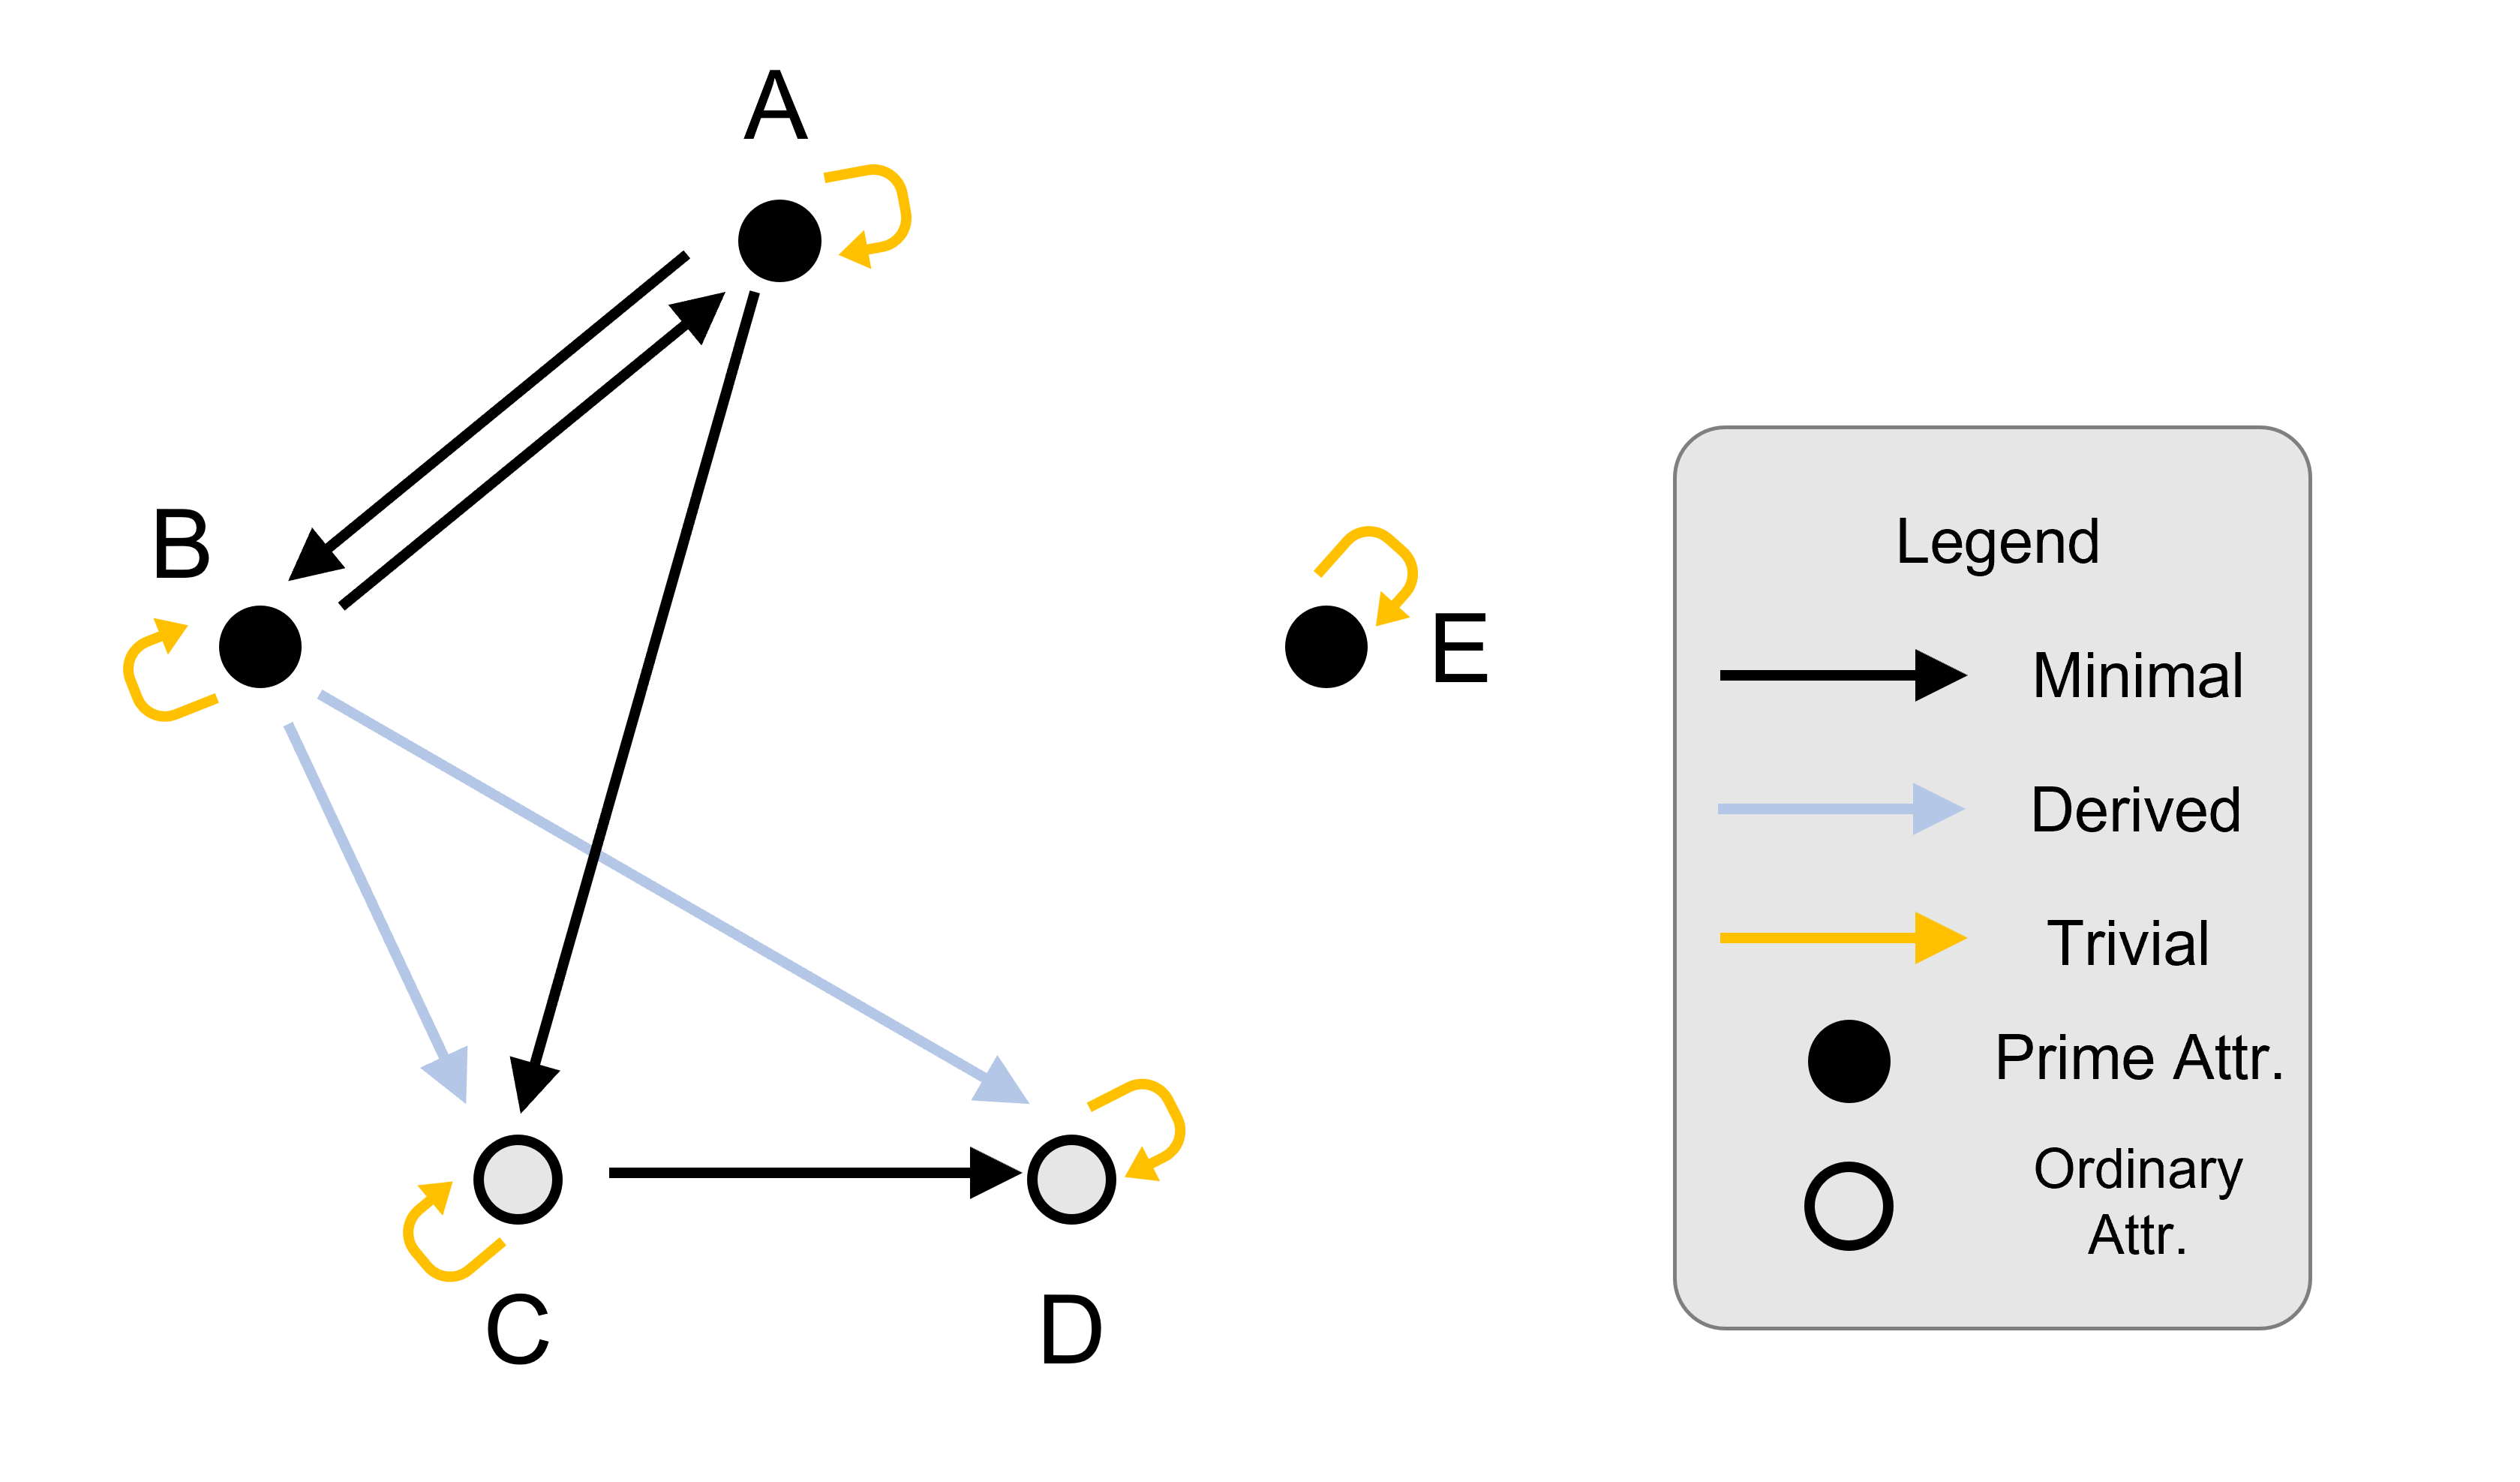
\includegraphics[width=0.85\textwidth, trim=0 0 0 0, clip]{t5/images/end_q1.png}
\end{figure}

\textit{(We will keep using this (kind of) figures for later demonstrations)}
\end{frame}

\begin{frame}[fragile]{Question 1 (b-c) Normal Forms}
(*) Is $R$ with $\Sigma$ in 2NF? (Just for recap purpose)\\\vspace{10pt}
(b) Is $R$ with $\Sigma$ in 3NF?\\\vspace{10pt}
(c) Is $R$ with $\Sigma$ in BCNF?\\\vspace{10pt}
\end{frame}

\begin{frame}[fragile]{Question 1 (b-c) Cont.}
(*) Is $R$ with $\Sigma$ in 2NF?\\\vspace{10pt}

\textbf{Recap}: How to \textcolor{brown}{mechanically} define 2NF?\\\vspace{10pt}
A relation $R$ with a set of functional dependencies $\Sigma$ is in second norm form (2NF) if and only iff for every functional dependency $X\rightarrow\{A\}$, we have:
\begin{itemize}
	\item $X\rightarrow\{A\}$ is trivial, or
	\item $X$ is not a subset of a candidate key, or
	\item $A$ is a prime attribute.
\end{itemize}\vspace{10pt}

\begin{alertblock}{Just to understand, no need to keep it in mind!}
	Unlike the 1NF that allow any attribute as long as they are single values, 
	The 2NF is more strict so that it does not allow any non-prime attribute to be determined by partial (not full) candidate keys.
\end{alertblock}

\end{frame}

\begin{frame}[fragile]{Question 1 (b-c) Cont.}
\begin{figure}
	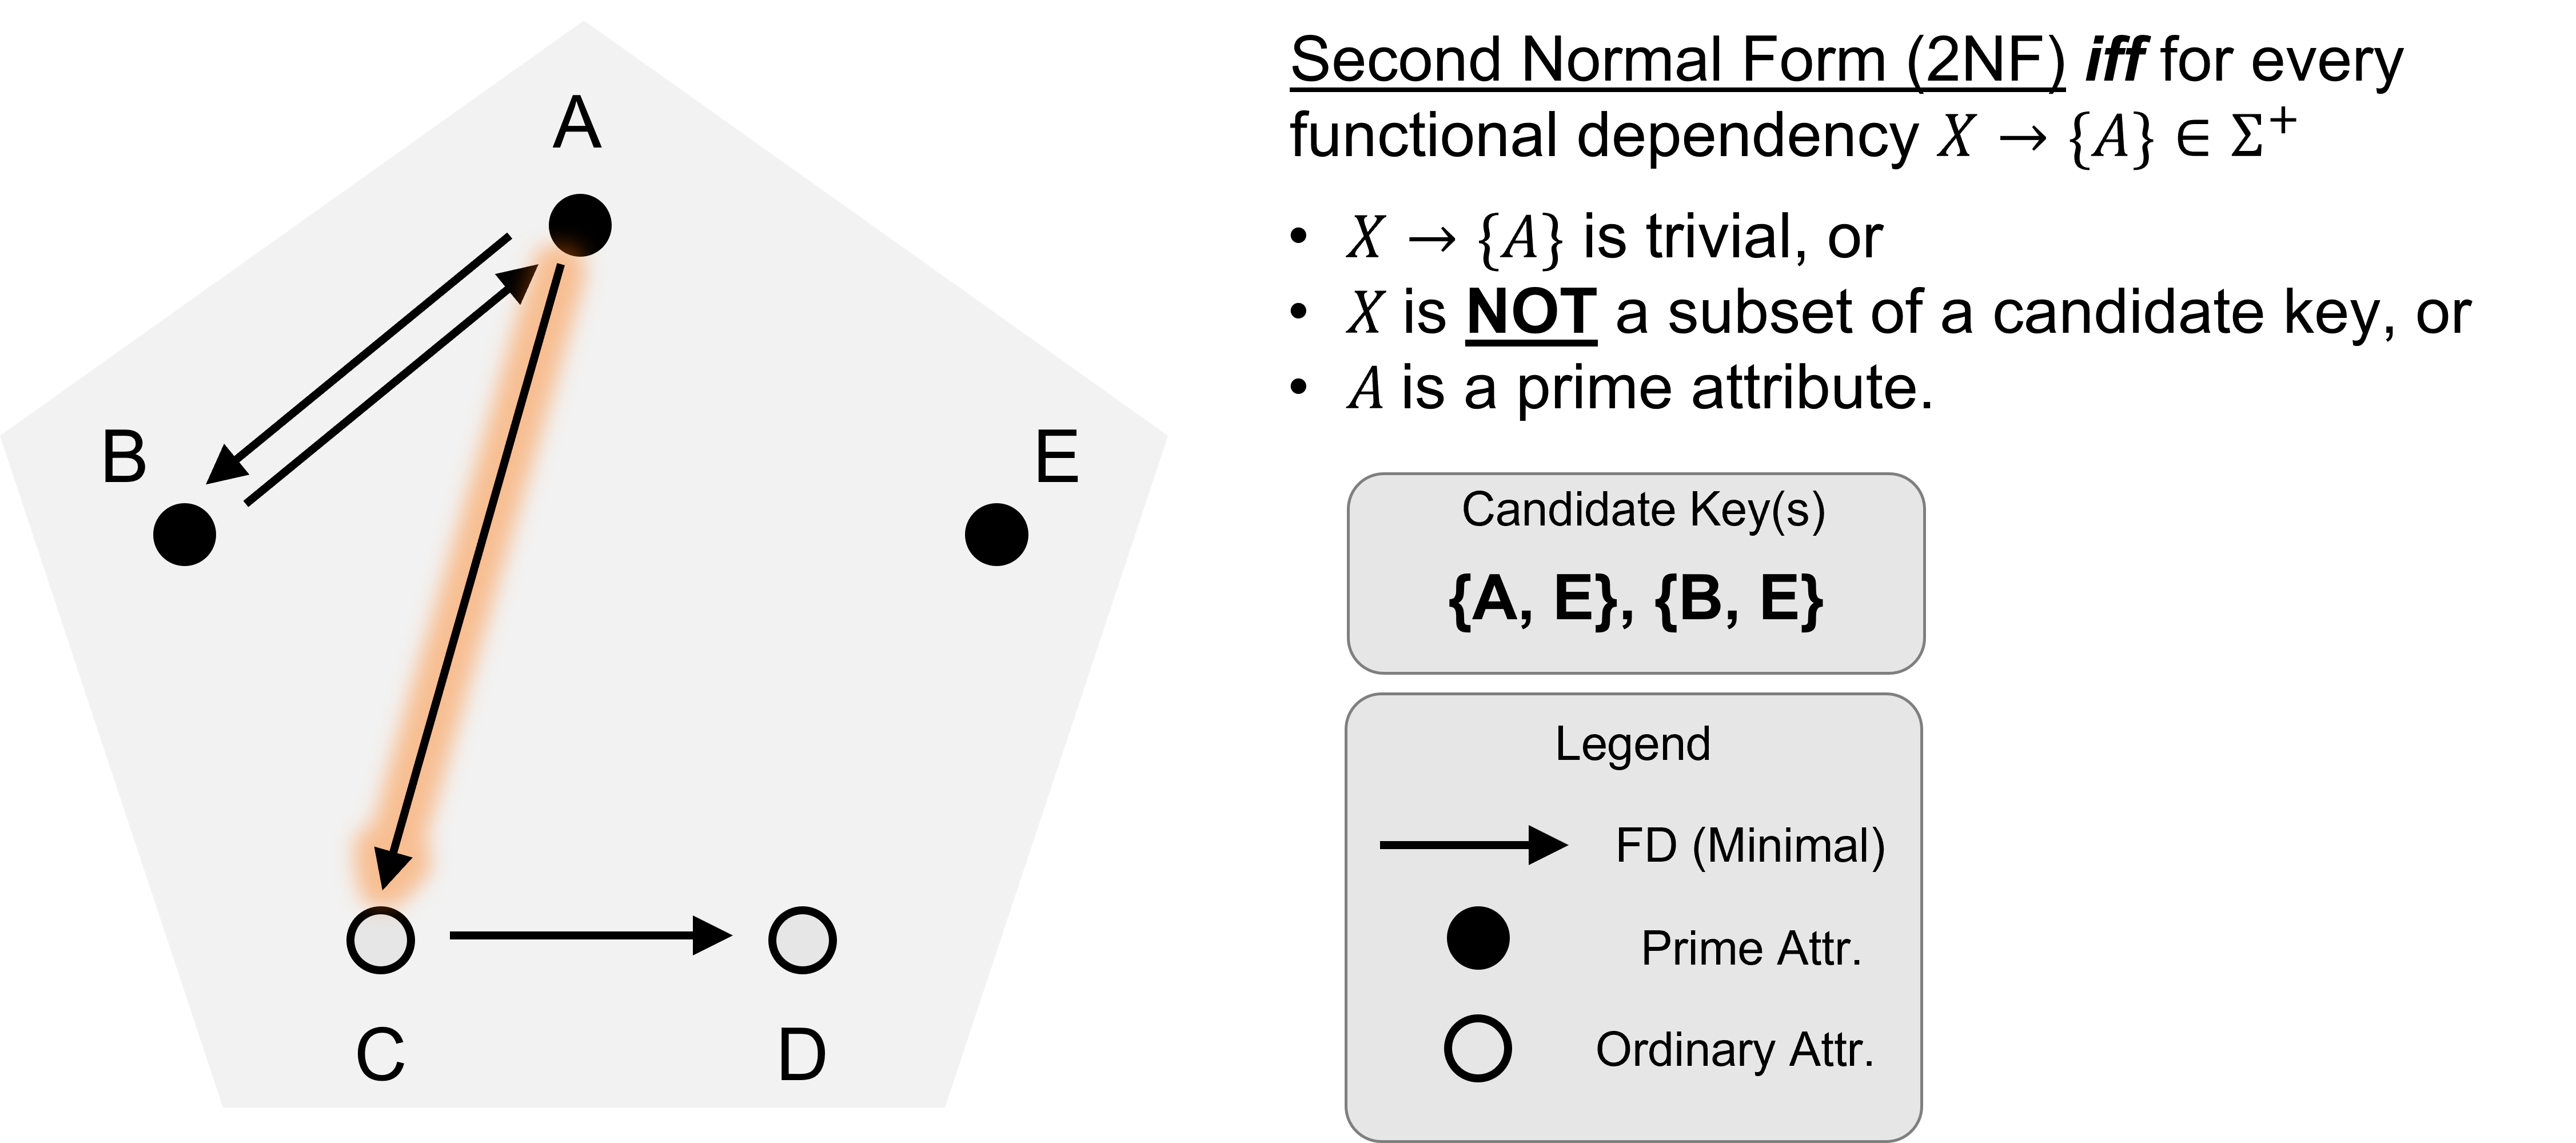
\includegraphics[width=0.85\textwidth, trim=0 0 0 0, clip]{t5/images/q3_2nf_highlight.png}
\end{figure}
\end{frame}

\begin{frame}[fragile]{Question 1 (b-c) Cont.}
\textbf{Solution}:
Let us look at the non-trivial functional dependencies of the form $X \rightarrow \{A\}$ derived from $\Sigma$. Namely after removing the trivial functional dependencies after step 1 of the minimal cover algorithm. Equivalently, we could use a minimal cover.\\\vspace{3pt}
$\{A\} \rightarrow \{C\}$ is non-trivial, $\{A\}$ is a proper subset of a candidate key and $\{C\}$ is not a prime attribute. This functional dependency violates the three conditions of the 2NF definition. $R$ with $\Sigma$ is not in 2NF.\\\vspace{3pt}

Incidentally, several other functional dependencies also violate the 2NF definition:\\
$\{B\} \rightarrow \{C\}$ is non-trivial, $\{B\}$ is a proper subset of a candidate key and $\{C\}$ is not a prime attribute. \\\vspace{3pt}
This ones do not (one condition is met):\\
$\{B,C\} \rightarrow \{D\}$ $\{B,C\}$ is not a proper subset of a candidate key.\\
$\{C\} \rightarrow \{D\}$ $\{C\}$ is not a proper subset of a candidate key.\\
$\{A\} \rightarrow \{B\}$ $\{B\}$ is a prime attribute.\\
$\{B, C\} \rightarrow \{A\}$ $\{A\}$ is a prime attribute.
\end{frame}

\begin{frame}[fragile]{Question 1 (b-c) Cont.}

(b) Is $R$ with $\Sigma$ in 3NF?\\\vspace{10pt}

\textbf{Recap}: How to \textcolor{brown}{mechanically} define 3NF?\\\vspace{10pt}
A relation $R$ with a set of functional dependencies $\Sigma$ is in third norm form (3NF) if and only iff for every functional dependency $X\rightarrow\{A\}$, we have:
\begin{itemize}
	\item $X\rightarrow\{A\}$ is trivial, or
	\item $X$ is a superkey, or
	\item $A$ is a prime attribute.
\end{itemize}\vspace{5pt}

\begin{alertblock}{Just to understand, no need to keep it in mind!}
	Unlike the 2NF that still allows a non-prime attribute to be determined by another non-prime attribute.\\ 
	The 3NF is more strict so that it does not allow any non-prime attribute to be determined by other non-prime attributes (all non-prime attributes have to be independent to each other, and therefore can only be determined by prime attributes).
\end{alertblock}

\end{frame}

\begin{frame}[fragile]{Question 1 (b-c) Cont.}
\begin{figure}
	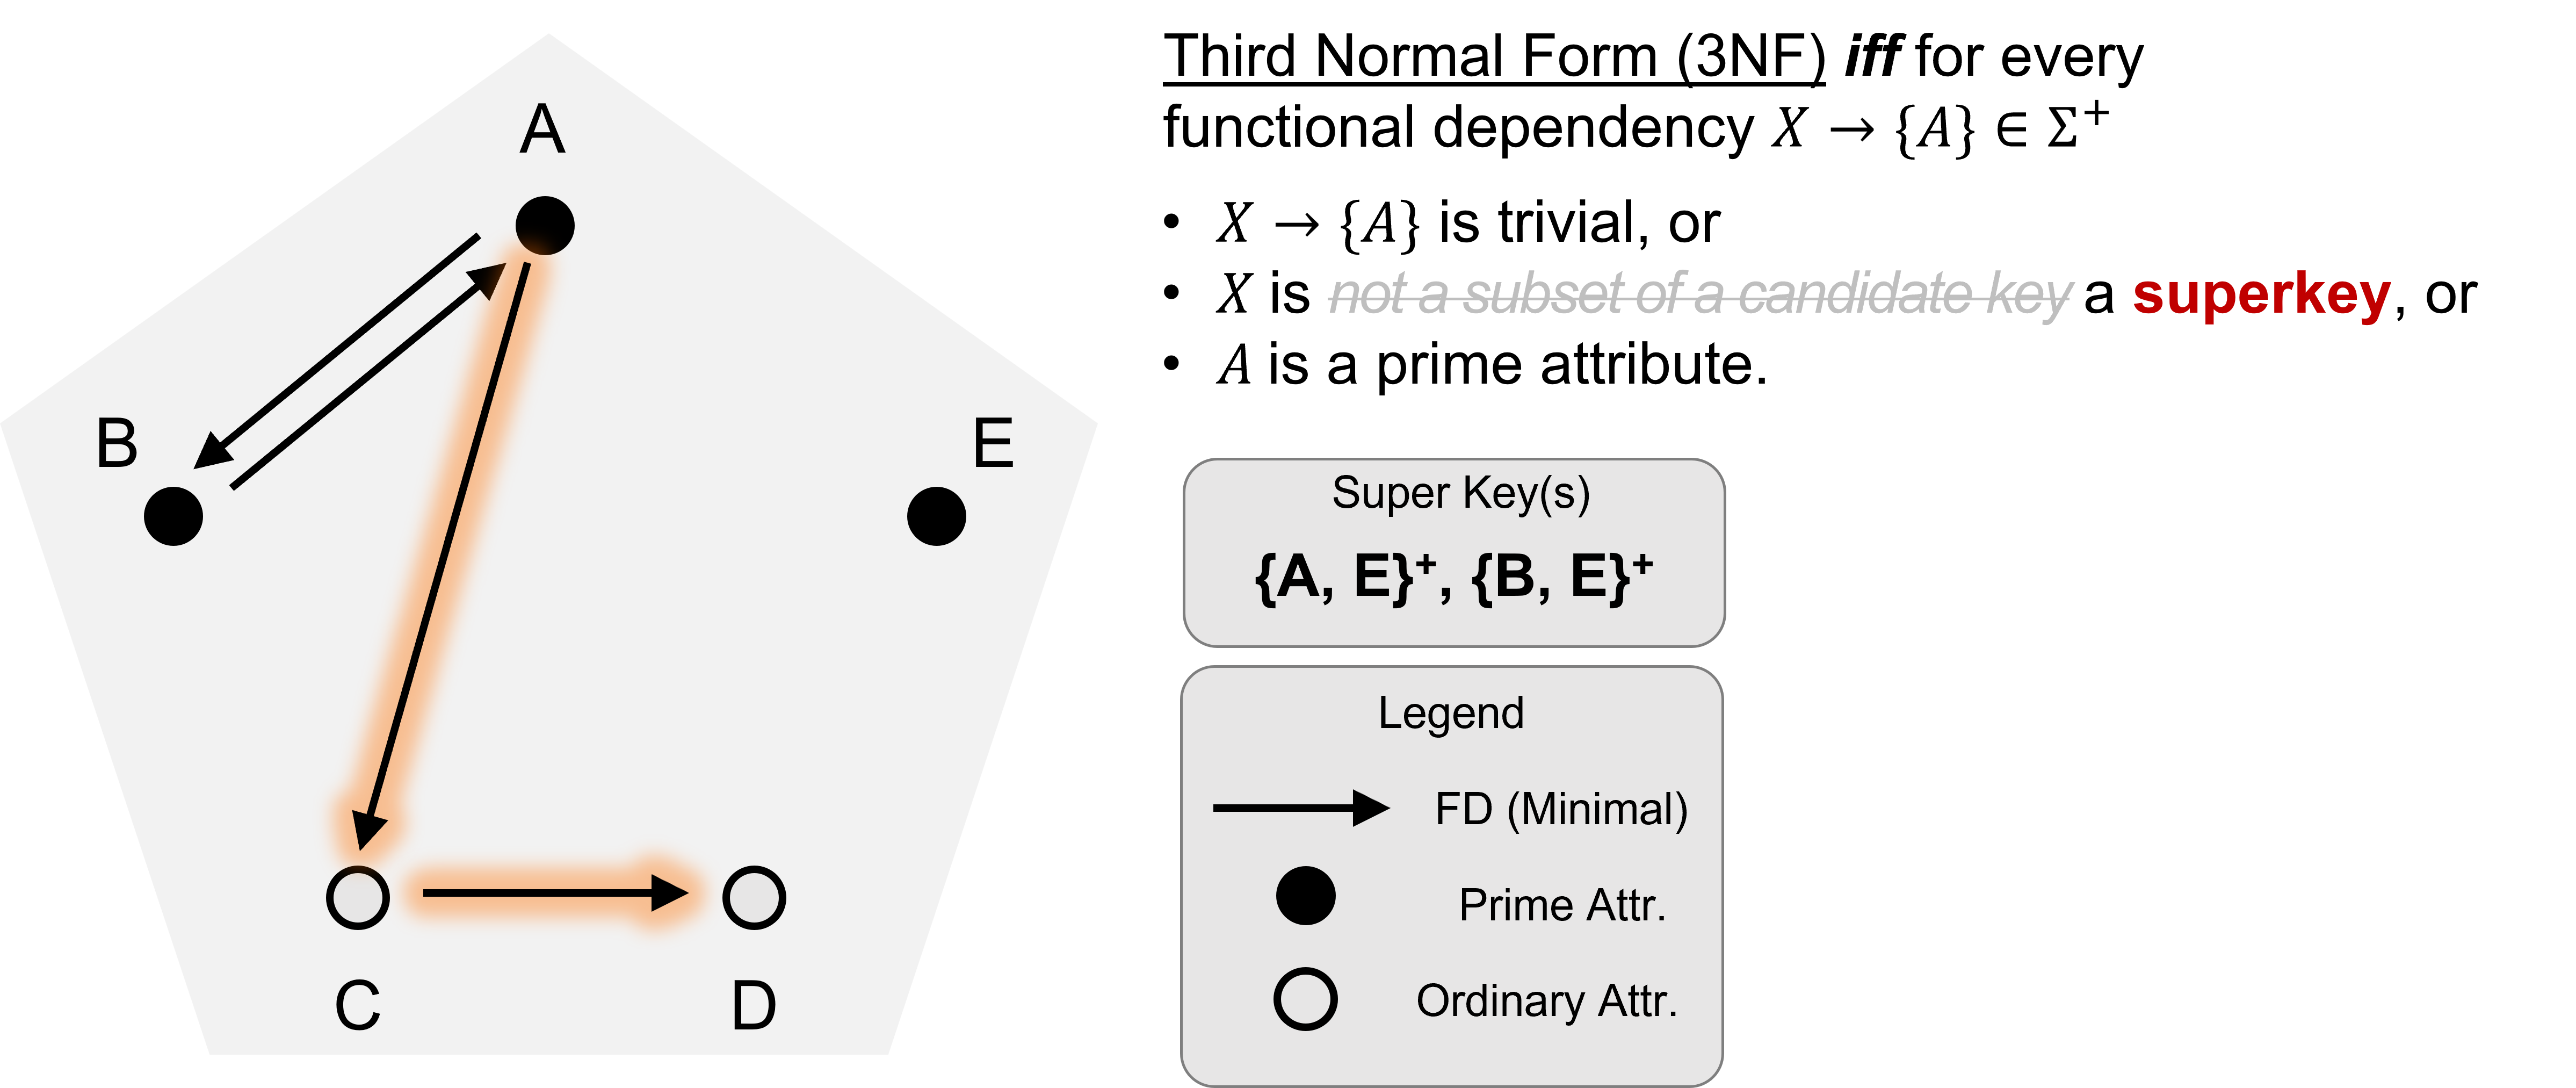
\includegraphics[width=0.95\textwidth, trim=0 0 0 0, clip]{t5/images/q3_3nf_highlight.png}
\end{figure}
\end{frame}

\begin{frame}[fragile]{Question 1 (b-c) Cont.}
\textbf{Solution}:
Let us look at the non-trivial functional dependencies of the form $X \rightarrow \{A\}$ derived from $\Sigma$. Namely after removing the trivial functional dependencies after step 1 of the minimal cover algorithm. Equivalently, we could use a minimal cover.\\\vspace{3pt}
$\{A\} \rightarrow \{C\}$ is non-trivial, $\{A\}$ is not a superkey and $\{C\}$ is not a prime attribute. This functional dependency violates the three conditions of the 3NF definition. $R$ with $\Sigma$ is not in 3NF.\\\vspace{3pt}

\end{frame}

\begin{frame}[fragile]{Question 1 (b-c) Cont.}
Incidentally, several other functional dependencies also violate the 3NF definition:\\

$\{B, C\} \rightarrow \{D\}$ is non-trivial, $\{B, C\}$ is not a superkey and $\{D\}$ is not a prime attribute.\\
$\{B\} \rightarrow \{C\}$ is non-trivial, $\{B\}$ is not a superkey and $\{C\}$ is not a prime attribute.\\
$\{C\} \rightarrow \{D\}$ is non-trivial, $\{C\}$ is not a superkey and $\{D\}$ is not a prime attribute.\\\vspace{10pt}

This two do not (one condition is met):\\
$\{A\} \rightarrow \{B\}$ is non-trivial, $\{A\}$ is not a superkey but $\{B\}$ is a prime attribute.\\\vspace{3pt}
$\{B, C\} \rightarrow \{A\}$ $\{A\}$ is a prime attribute.\\\vspace{3pt}

\end{frame}

\begin{frame}[fragile]{Question 1 (b-c) Cont.}
(c) Is $R$ with $\Sigma$ in BCNF?\\\vspace{10pt}

\textbf{Recap}: How to \textcolor{brown}{mechanically} define BCNF?\\\vspace{10pt}
A relation $R$ with a set of functional dependencies $\Sigma$ is in Boyce-Codd norm form (BCNF) if and only iff for every functional dependency $X\rightarrow\{A\}$, we have:
\begin{itemize}
	\item $X\rightarrow\{A\}$ is trivial, or
	\item $X$ is a superkey.
\end{itemize}\vspace{3pt}

\begin{alertblock}{Just to understand, no need to keep it in mind!}
BCNF was proposed in 1974 (3 years later than 2NF and 3NF) and was known as 3.5NF at the beginning.\\\vspace{3pt}
Unlike the 3NF that does not allow a non-prime attribute to be determined by other non-prime attributes (e.g. \texttt{city} is determined by \texttt{postal} in a database that record residence details). 
The BCNF is more strict so that it only allow attribute(s) to be determined by superkeys.
\end{alertblock}

\end{frame}

\begin{frame}[fragile]{Question 1 (b-c) Cont.}
\begin{figure}
	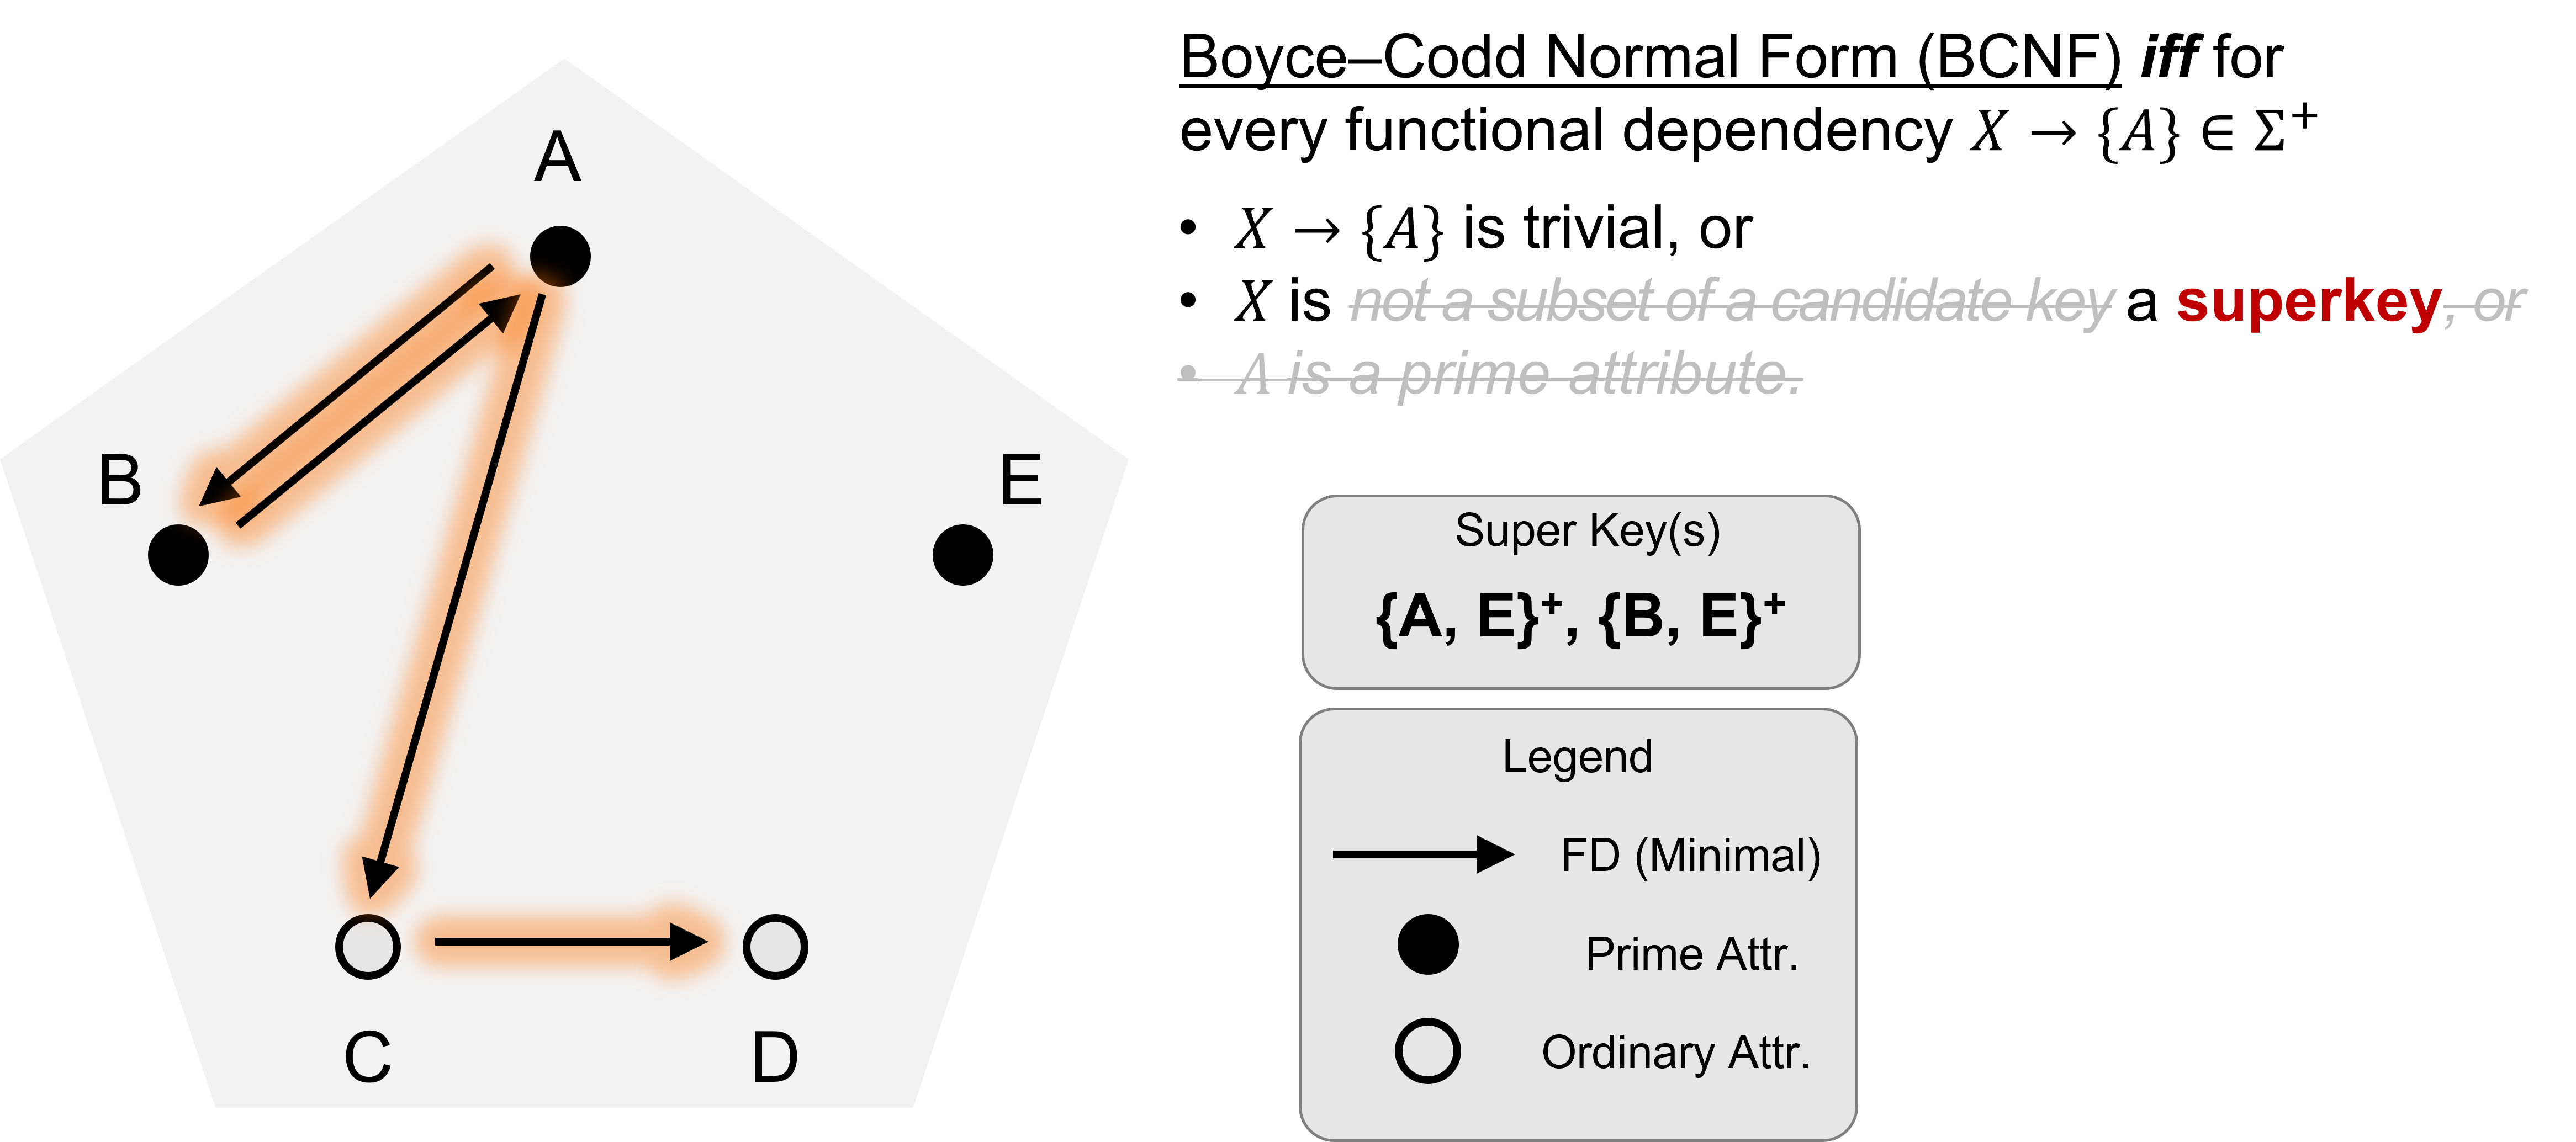
\includegraphics[width=0.85\textwidth, trim=0 0 0 0, clip]{t5/images/q3_bcnf_highlight.png}
\end{figure}
\end{frame}

\begin{frame}[fragile]{Question 1 (b-c) Cont.}
\textbf{Solution}:
$R$ with $\Sigma$ is not in 3NF, then it cannot be in BCNF.\\\vspace{3pt}

Let us look at the non-trivial functional dependencies of the form $X \rightarrow \{A\}$ derived from $\Sigma$. Namely after removing the trivial functional dependencies after step 1 of the minimal cover algorithm. Equivalently, we could use a minimal cover.\\\vspace{3pt}

$\{A\} \rightarrow \{C\}$ is non-trivial and $\{A\}$ is not a superkey . This functional dependency violates the two conditions of the BCNF definition. $R$ with $\Sigma$ is not in BCNF.\\\vspace{3pt}

Incidentally, all the other functional dependencies also violate the BCNF definition:\\
$\{A\} \rightarrow \{B\}$ is non-trivial and $\{A\}$ is not a superkey.\\
$\{B, C\} \rightarrow \{D\}$ is non-trivial and $\{B, C\}$ is not a superkey.\\
$\{B\} \rightarrow \{C\}$ is non-trivial and $\{B\}$ is not a superkey.\\
$\{C\} \rightarrow \{D\}$ is non-trivial and  $\{C\}$ is not a superkey.\\
$\{B, C\} \rightarrow \{A\}$ $\{A\}$ is non-trivial and  $\{B, C\}$ is not a superkey.
\end{frame}

\begin{frame}[fragile]{Question 1 (d-j) Normalisation}
	(d) Decompose $R$ with $\Sigma$ into a BCNF decomposition using the algorithm from the lecture.\\\vspace{5pt}
	
	\textbf{Solution}: We found that $\{A\} \rightarrow \{C\}$ violates the BCNF condition.\\\vspace{3pt}
	
	We use it to decompose into two fragments:\\
	$R_1 = \{A\}^{+} = \{A, B, C, D\}$ with $\Sigma_1 = \{\{A\} \rightarrow \{C\}, \{A\} \rightarrow \{B\},\{B\} \rightarrow \{A\}, \{C\} \rightarrow \{D\}\}$.
	
	$R_2 = \{A, E\}$ with $\Sigma_2 = \emptyset$.
	
	$R_2$ with $\Sigma_2$ is in BCNF.
	
	$R_1$ with $\Sigma_1$ is not in BCNF because $\{C\} \rightarrow \{D\}$ violates the BCNF condition.
	\textbf{$\leftarrow$ We need to further decompose it.}
\end{frame}

\begin{frame}[fragile]{Question 1 (d-j) Cont.}
	For $R_1 = \{A\}^{+} = \{A, B, C, D\}$, we use it to decompose into two fragments:\\\vspace{5pt}
	$R_{1.1} = \{C\}^{+} = \{C, D\}$ (computed for $R_1$ with $\Sigma_1$!) with $\Sigma_{1.1} = \{\{C\} \rightarrow \{D\}\}$.
	
	$R_{1.2} = \{A, B, C\}$ with $\Sigma_{1.2} = \{\{A\} \rightarrow \{B\}, \{A\} \rightarrow \{C\}, \{B\} \rightarrow \{A\}\}$.\\\vspace{5pt}
	
	$R_{1.1}$ with $\Sigma_{1.1}$ is in BCNF.
	
	$R_{1.2}$ with $\Sigma_{1.2}$ is in BCNF.\\\vspace{5pt}
	
	The result is a decomposition into three fragments: $R_2$, $R_{1.1}$ and $R_{1.2}$.\\\vspace{5pt}
\end{frame}

\begin{frame}[fragile]{Question 1 (d-j) Cont.}
	(e) Is the results lossless?\\\vspace{5pt}
	\textbf{Solution}: Yes, the algorithm guarantees that the result is lossless.\\
	\vspace{30pt}
	(f) Is the results dependency preserving?\\\vspace{5pt}
	\textbf{Solution}:
	Incidentally yes, the \textbf{algorithm} (itself) \textcolor{red}{\textbf{does not}} guarantee that the result is dependency preserving.\\
	\begin{alertblock}{Notice}
		Don't take the dependency preserving for granted in decomposition.
	\end{alertblock}
	
\end{frame}

\begin{frame}[fragile]{Question 1 (d-j) Cont.}
(g) Synthesise $R$ with $\Sigma$ into a 3NF decomposition using the algorithm from the lecture.\\\vspace{5pt}

\textbf{Solution}:
First compute a compact minimal cover:

$\{A\} \rightarrow \{B, C\}$

$\{B\} \rightarrow \{A\}$

$\{C\} \rightarrow \{D\}$

For each functional dependency create a fragment:

$R_1 = \{A, B, C\}$

$R_2 = \{B, A\}$ , this fragment is not kept: it is subsumed by $R_1$.

$R_3 = \{C, D\}$.

None of the fragments contain a candidate key. We choose one: say $\{A, E\}$, and add it as fragment:

$R_4 = \{A, E\}$.

The result is:
$R_1 = \{\underline{A}, \underline{B}, C\}$
$R_3 = \{\underline{C}, D\}$.
$R_4 = \{\underline{A, E}\}$.

The algorithm always works. It is guaranteed to find a decomposition in 3NF. Note that using a different minimal cover or compact minimal cover may give a different (but equally correct) result.
\end{frame}

\begin{frame}[fragile]{Question 1 (d-j) Cont.}
(h) Is the results lossless?\\\vspace{5pt}
\textbf{Solution}: Yes, the algorithm guarantees that the result is lossless.
\\\vspace{30pt}
(i) Is the results dependency preserving?\\\vspace{5pt}
\textbf{Solution}:
Yes, the algorithm guarantees that the result is dependency preserving.

\end{frame}

\begin{frame}[fragile]{Question 1 (d-j) Cont.}
(j) Is the results in BCNF?\\\vspace{5pt}

\textbf{Solution}:
The algorithm guarantees that the result is in 3NF. In this case, it is also in BCNF! (you can check). It is not always but often the case.\\\vspace{10pt}

\textcolor{red}{\textbf{Extra}}:\\
To wrap-up, BCNF decomposition is \textbf{not always optimal}, as it aims to dismiss some ``unnecessary'' dependencies among attributes. (sometimes 3NF is good enough)\\\vspace{5pt}
\end{frame}


\begin{frame}{}
	\begin{figure}
		
\includegraphics[width=0.6\textwidth, trim=0 3.5cm 0 0, clip]{t5/images/final.png}
	\end{figure}
\begin{center}
	Enjoy the recess week and have a good rest. Keep safe!
\end{center} 
\end{frame}

\begin{frame}{}
	\centering  
	For any further question, please feel free to email me:\vspace{10pt}
	
	huasong.meng@u.nus.edu\\\vspace{3pt}
	%menghs@i2r.a-star.edu.sg (work)\\\vspace{3pt}
	%huasong.meng@gmail.com (personal)\vspace{10pt}
	
	Or you can whatsapp/wechat me via: 81028639 \vspace{20pt}
	
	\begin{tcolorbox}
		\begin{center}
			\textcolor{red}{Copyright 2021 Mark H. Meng. All rights reserved.}
		\end{center}
	\end{tcolorbox}
\end{frame}
%\title{CS4221/CS5421}

\subtitle{Tutorial 5: Dependencies, entity-relationship modelling and the Chase}

\author{Mark Meng Huasong}

\institute[National University of Singapore] % (optional, but mostly needed)
{
	School of Computing\\
	National University of Singapore
}

\titlegraphic{
	
\includegraphics[width=2cm]{nus-logo}
}

\date{Week 7, 2022 Spring}

\begin{frame}
	\titlepage
	\begin{tcolorbox}
		\begin{center}
			{\scriptsize \textcolor{red}{All the materials within presentation slides are protected by copyrights.\\
					It is forbidden by NUS to upload these materials to the Internet.}}
		\end{center}
	\end{tcolorbox}
\end{frame}

\section*{Question 1 Entity-relationship Design}

\begin{frame}[fragile]{Question 1 Entity-relationship Design}
Consider the entity-relationship diagram of Figure 1.
\begin{figure}
	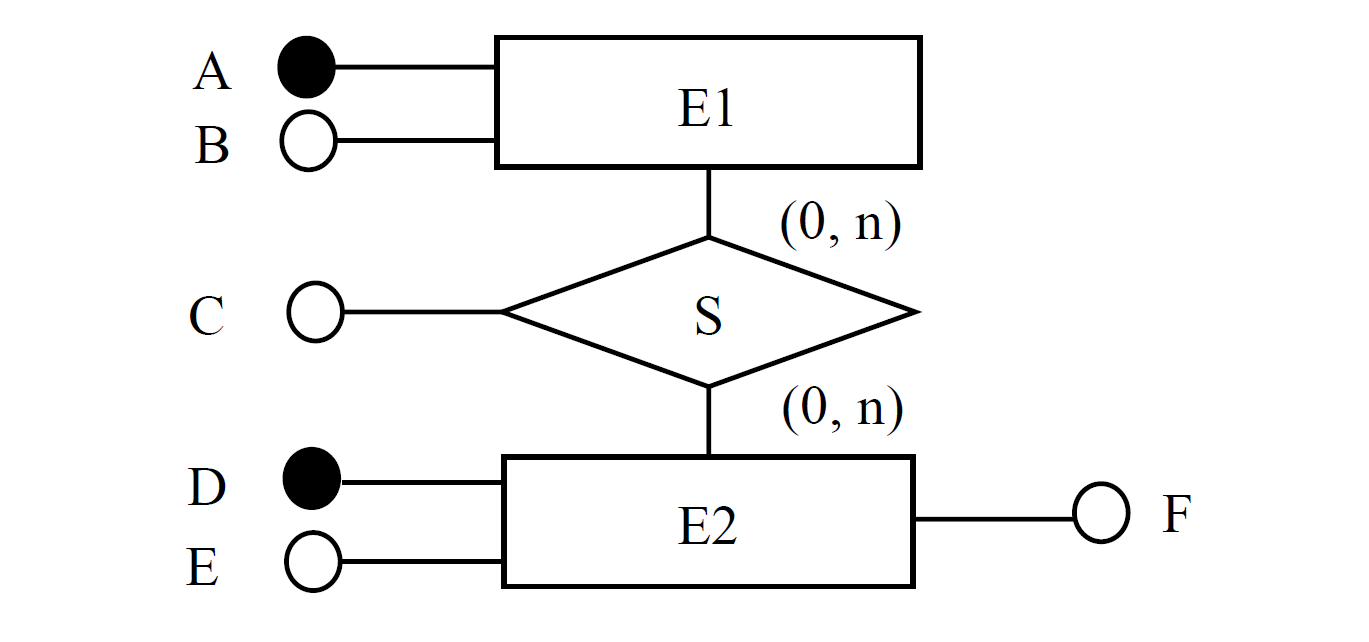
\includegraphics[width=0.75\textwidth, trim=0 0 0 0, clip]{4221-t5/images/q1.png}
\end{figure}
(a) Without other knowledge than that captured by the entity-relationship diagram, what are the \textbf{functional} and \textbf{multi-valued} dependencies?
\end{frame}

\begin{frame}[fragile]{Question 1 (Cont.)}
\textbf{Solution}: The entity-relationship diagram tells us the following functional dependencies.\\ \vspace{5pt}

$\Sigma = \{\{A\}\rightarrow\{B\}, \{D\}\rightarrow\{E,F\}, \{A,D\}\rightarrow\{C\}\}$
\\ \vspace{10pt}

Multi-valued dependencies depend on the translation of this design into tables. The entity-
relationship diagram and its translation will only result in ``not interesting'' multi-valued dependencies, those are trivial or correspond to the table or the functional dependencies.\\ \vspace{5pt}
If we canonically translate this design into three tables, we have
$\{A\} \twoheadrightarrow \{B\}$ and $\{C\}\twoheadrightarrow \{A,D\}$ and many more (none of them being useful for normalisation), for instance.
\end{frame}

\begin{frame}[fragile]{Question 1 (Cont.)}
	
Note that additional knowledge of the application could tell us additional functional and multivalued dependencies not captured by the design.\\ \vspace{5pt}

For instance, we could know that $\{E\}\rightarrow\{F\}$ (which would suggest that the entity-relationship design is probably missing entities and relationships that have been merged too early), which we could use to produce a design in the Boyce-Codd normal by splitting the table $R_3(D,E,F)$ into two tables $R_{3.1}=(\underline{D},E)$ and $R_{3.2}=(\underline{E},F)$.\\ \vspace{5pt}

For instance, we could know that $\{E\}\twoheadrightarrow\{F\}$, which we could use to produce a design in the fifth normal by splitting the table $R_3(D,E,F)$ into two tables $R_{3.1}=(\underline{D},E)$ and $R_{3.2}=(\underline{E,F})$.	
\end{frame}

\section*{Question 2 MVD \& Chase}

\begin{frame}[fragile]{Question 2 MVD}
Consider the relational schema $R = \{A,B,C,D,E\}$ with the following set of functional and multi-valued dependencies.\\ \vspace{5pt}

$\Sigma=\{\{C\}\rightarrow\{A\}, \{D\}\rightarrow\{D,B\}, \{B\}\rightarrow\{E\},\{E\}\twoheadrightarrow\{A,D\},\{A,B,D\}\rightarrow\{A,B,C,D\},\{B\}\rightarrow\{D\}\}$\\ \vspace{5pt}

(a) Prove that $\{E\}\rightarrow\{D\}$ using the Armstrong and multi-valued dependencies axioms.\\ \vspace{5pt}

\textbf{Solution:}\\ \vspace{5pt}
1. We know that $\{E\}\twoheadrightarrow\{A,D\}$.\\ \vspace{2pt}
2. We know that $\{B\}\rightarrow\{D\}$.\\\vspace{2pt}
3. We see that $\{D\}\subset\{A,D\}$.\\\vspace{2pt}
4. We see that $\{B\}\cap \{A,D\}=\emptyset$\\\vspace{2pt}
5. Therefore $\{E\}\rightarrow\{D\}$ by Coalescence of (1), (2), (3) and (4).\\\vspace{2pt}
\hfill Q.E.D.\\\vspace{10pt}
Try the same question with the Chase (answer not provided).
\end{frame}

\begin{frame}[fragile]{Question 3 Chase}
Consider the relation $R(A,B,C,D,E,G)$ with the following set, $F$, of functional and multi-valued dependencies.\\ \vspace{5pt}
	
$F=\{\{A,B\}\rightarrow\{C\}, \{A,B\}\twoheadrightarrow\{E\},\{C,D\}\twoheadrightarrow\{A,B\}\}$\\ \vspace{5pt}
	
Prove that the decomposition of $R$ into $R_1(A,B,C,D,G)$ and $R_2(C,D,E)$ is lossless using the Chase algorithm (as shown in the lecture).\\ \vspace{5pt}

\textbf{\textcolor{blue}{How to solve this question?}}\\\vspace{5pt}
\textcolor{blue}{Recall the lecture note ``\emph{Testing if a decomposition is lossless}''.
We first analyze the decomposition to find out what is the $X$ of ``$R=X\cup Y\cup Z$''. We have $X=\{C,D\}$.\\\vspace{2pt}
Then we need to use the Chase method to chase $\{C,D\}\twoheadrightarrow\{E\}$ ({\small or $\{C,D\}\twoheadrightarrow\{A,B,G\}$ equivalently, according to Complementation rule of Armstrong Axiom}).}\\\vspace{5pt}

\textcolor{blue}{Now the question becomes:\\
$\{\{A,B\}\rightarrow\{C\}, \{A,B\}\twoheadrightarrow\{E\},\{C,D\}\twoheadrightarrow\{A,B\}\} \models \{C,D\}\twoheadrightarrow\{E\}$?.}
\end{frame}

\begin{frame}[fragile]{Question 3 (Cont.)}	
\textbf{Solution:}\\ \vspace{2pt}
1. Initial table.\\
\begin{figure}
	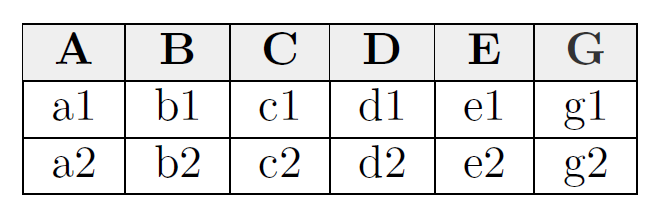
\includegraphics[width=0.4\textwidth, trim=0 0 0 0, clip]{4221-t5/images/3-1.png}
\end{figure}

2. We want to chase $\{C,D\} \twoheadrightarrow \{E\}$, make $C$ and $D$ values the same.\\
\begin{figure}
	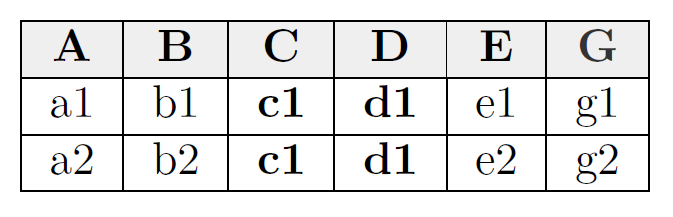
\includegraphics[width=0.4\textwidth, trim=0 0 0 0, clip]{4221-t5/images/3-2.png}
\end{figure}

\end{frame}

\begin{frame}[fragile]{Question 3 (Cont.)}
3. Apply $\{C,D\} \twoheadrightarrow \{A,B\}$ by copying two tuples that have the same $C$ and $D$ values but swapping their $A$ and $B$ values.\\\vspace{10pt}

\textcolor{blue}{{\small Below are cited from the ``Chasing the Chase'' part of the lecture note:\\\vspace{5pt}
\textit{For each multi-valued dependency $Z\twoheadrightarrow V\in\Sigma$, if there are 2 tuples in the table with the \textbf{SAME $Z$-value}, then add two new tuples with \textbf{all the same values and except} for their $V$-values that are \textbf{SWAPPED}.}}}

\begin{figure}
	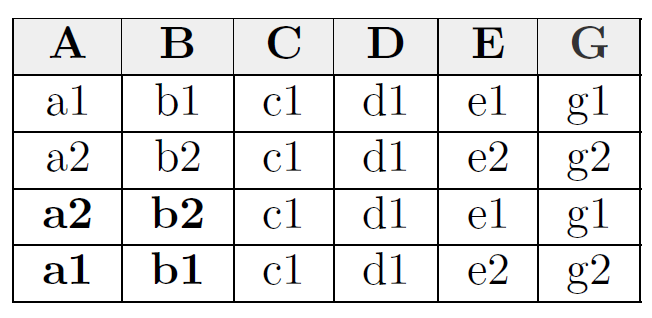
\includegraphics[width=0.4\textwidth, trim=0 0 0 0, clip]{4221-t5/images/3-3.png}
\end{figure}

\end{frame}


\begin{frame}[fragile]{Question 3 (Cont.)}
4. Apply $\{A,B\} \twoheadrightarrow \{E\}$ by copying two tuples that have the same $A$ and $B$ values but swapping their $A$ and $E$ values.\\
\begin{figure}
	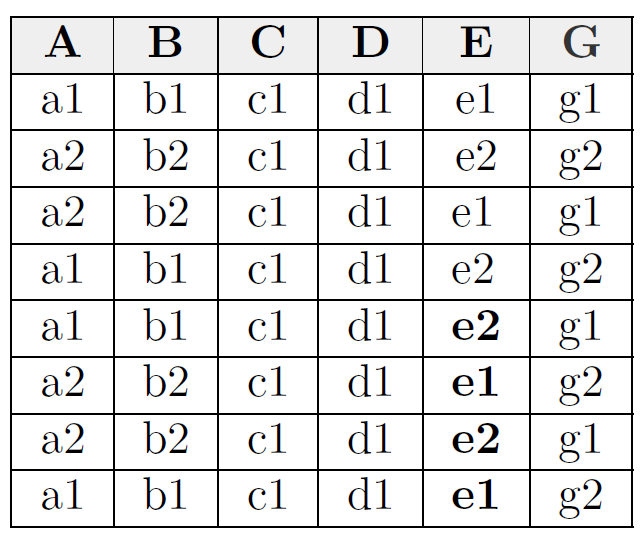
\includegraphics[width=0.4\textwidth, trim=0 0 0 0, clip]{4221-t5/images/3-4.png}
\end{figure}
\end{frame}


\begin{frame}[fragile]{Question 3 (Cont.)}
5. Applying $\{A,B\} \rightarrow \{C\}$ do not change the table.\\\vspace{5pt}
\textcolor{blue}{{\small \textit{Because we cannot find for any two tuples $\{a1,b1,c1,...\}$ and $\{a2,b2,c2,...\}$ s.t. $\{a1,b1\}=\{a2,b2\}$ but $c1 \ne c2$}.}}\\\vspace{10pt}

6. Sort the table and proved that $\{C,D\}\twoheadrightarrow\{E\}$ 
	\begin{figure}
		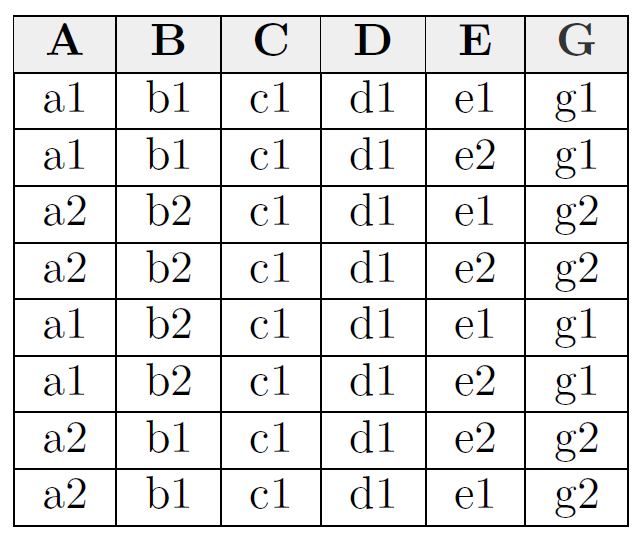
\includegraphics[width=0.4\textwidth, trim=0 0 0 0, clip]{4221-t5/images/3-6.png}
	\end{figure}

\textcolor{blue}{{\small \textit{Because we cannot find any counterexample.}}}\\\vspace{10pt}
	\hfill Q.E.D
\end{frame}


\begin{frame}[fragile]{Question 4 Chase}
	Consider the relation $R(A,B,C,D,E,F,G)$ with the following set, $\Sigma$, of functional dependencies.\\ \vspace{5pt}
	
	$\Sigma=\{\{A,B\}\rightarrow\{C\},\{C\}\rightarrow\{D,E\},\{E\}\rightarrow\{D\},\{F\}\rightarrow\{G\}\}$\\ \vspace{5pt}
	
	Prove that the decomposition of $R$ into $R_1(A,B,C,D,E)$ and $R_2(A,B,F,G)$ is lossless using the Chase algorithm (as shown in the lecture).\\ \vspace{5pt}
	
	\textbf{Solution:}\\ \vspace{2pt}
	1. Initial table.\\
	\begin{figure}
		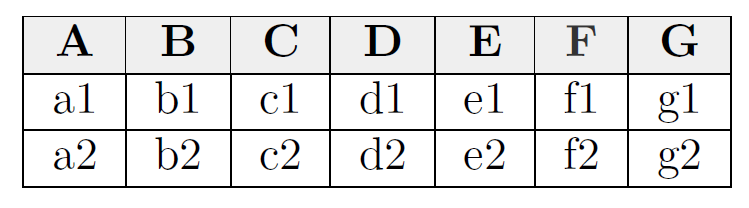
\includegraphics[width=0.4\textwidth, trim=0 0 0 0, clip]{4221-t5/images/4-1.png}
	\end{figure}
	
	2. We want to chase $\{A,B\} \twoheadrightarrow \{C,D,E\}$, make $A$ and $B$ values the same.\\
	\begin{figure}
		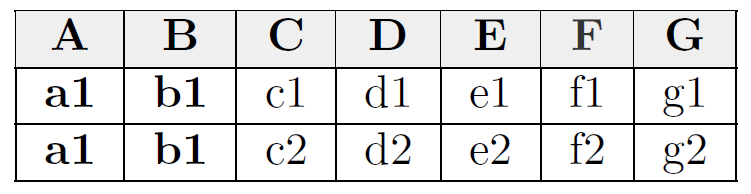
\includegraphics[width=0.4\textwidth, trim=0 0 0 0, clip]{4221-t5/images/4-2.png}
	\end{figure}	
\end{frame}

\begin{frame}[fragile]{Question 4 (Cont.)}
	3. Apply $\{A,B\} \rightarrow \{C\}$, make $C$ with the same $A$ and $B$ values the same.\\
	\begin{figure}
		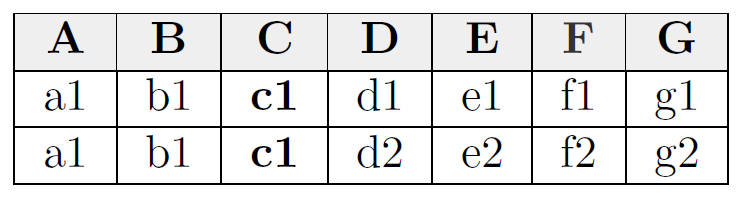
\includegraphics[width=0.4\textwidth, trim=0 0 0 0, clip]{4221-t5/images/4-3.png}
	\end{figure}
	
	4. Apply $\{C\} \rightarrow \{D,E\}$, make $D$ and $E$ with the same $C$ values the same.\\
	\begin{figure}
		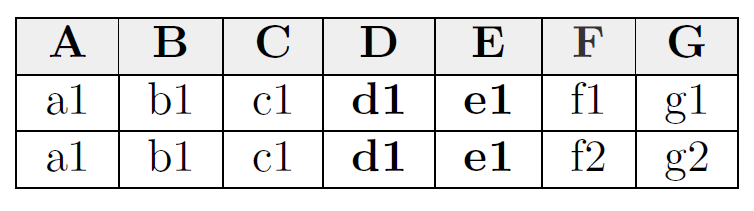
\includegraphics[width=0.4\textwidth, trim=0 0 0 0, clip]{4221-t5/images/4-4.png}
	\end{figure}

	5. Applying $\{E\} \rightarrow \{D\}$ does not change the table.\\\vspace{5pt}
	6. Applying $\{F\} \rightarrow \{G\}$ does not change the table.\\\vspace{5pt}
	7. Proved that $\{A,B\} \twoheadrightarrow \{C,D,E\}.$\\
	\hfill Q.E.D
	
\end{frame}


\begin{frame}[fragile]{Question 5 Chase with the Distinguished Attributes}
	Consider the relation $R(A,B,C,D,E)$ with the following set, $F$, of functional dependencies.\\ \vspace{5pt}
	
	$\Sigma=\{\{A\}\rightarrow\{B,C\}, \{B\}\rightarrow\{A\},\{C\}\rightarrow\{D\}\}$\\ \vspace{5pt}
	
	Check whether the decomposition of $R$ into $R_1(A,E)$, $R_2(C,D)$ and $R_3(A,B,C)$ is lossless using the Chase algorithm with the distinguished attributes.\\ \vspace{5pt}
	
	\textbf{Solution:}\\ \vspace{2pt}
	1. Initial table.\\
	\begin{figure}
		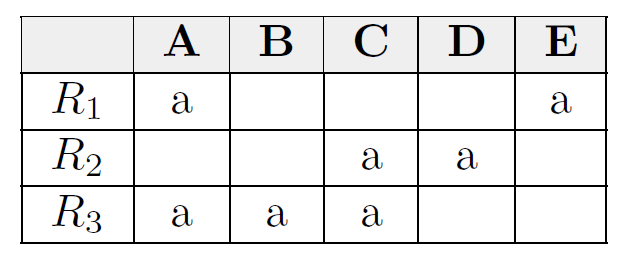
\includegraphics[width=0.3\textwidth, trim=0 0 0 0, clip]{4221-t5/images/5-1.png}
	\end{figure}
	
	2. Apply $\{A\} \rightarrow \{B,C\}$.\\
	\begin{figure}
		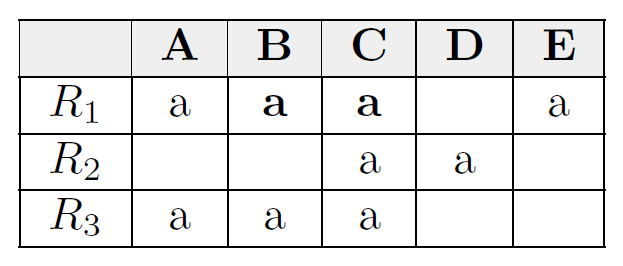
\includegraphics[width=0.3\textwidth, trim=0 0 0 0, clip]{4221-t5/images/5-2.png}
	\end{figure}
	
\end{frame}
\begin{frame}[fragile]{Question 5 (Cont.)}
	
	3. Applying $\{B\} \rightarrow \{A\}$ does not change the table.\\
	4. Apply $\{C\} \rightarrow \{D\}$.\\
	\begin{figure}
		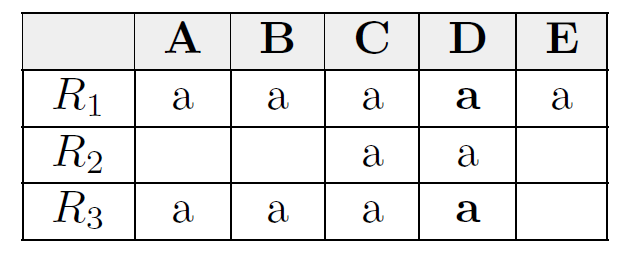
\includegraphics[width=0.3\textwidth, trim=0 0 0 0, clip]{4221-t5/images/5-4.png}
	\end{figure}

	5. $R_1$ has distinguished variables in all of the columns, therefore the decomposition is lossless.\\
	\hfill Q.E.D
\end{frame}

\section*{Extra Practice}
\begin{frame}[fragile]{Extra Practice (A): Chase}
\underline{Q2 Revisit}: consider the relational schema $R = \{A,B,C,D,E\}$ with the following set of functional and multi-valued dependencies.\\ \vspace{5pt}

$\Sigma=\{\{C\}\rightarrow\{A\}, \{D\}\rightarrow\{D,B\}, \{B\}\rightarrow\{E\},\{E\}\twoheadrightarrow\{A,D\},\{A,B,D\}\rightarrow\{A,B,C,D\},\{B\}\rightarrow\{D\}\}$\\ \vspace{5pt}

Prove that $\{E\}\rightarrow\{D\}$ using the \textbf{Chase algorithm}.\\ \vspace{5pt}
\end{frame}

\begin{frame}[fragile]{Extra Practice (B): ER Participation vs. Logical Design}
Can you spot the difference among the 4 cases below? Can you explain what they look like in the logical design? Can you give an example from the real world for each case?\\ \vspace{4pt}
	
\begin{figure}
	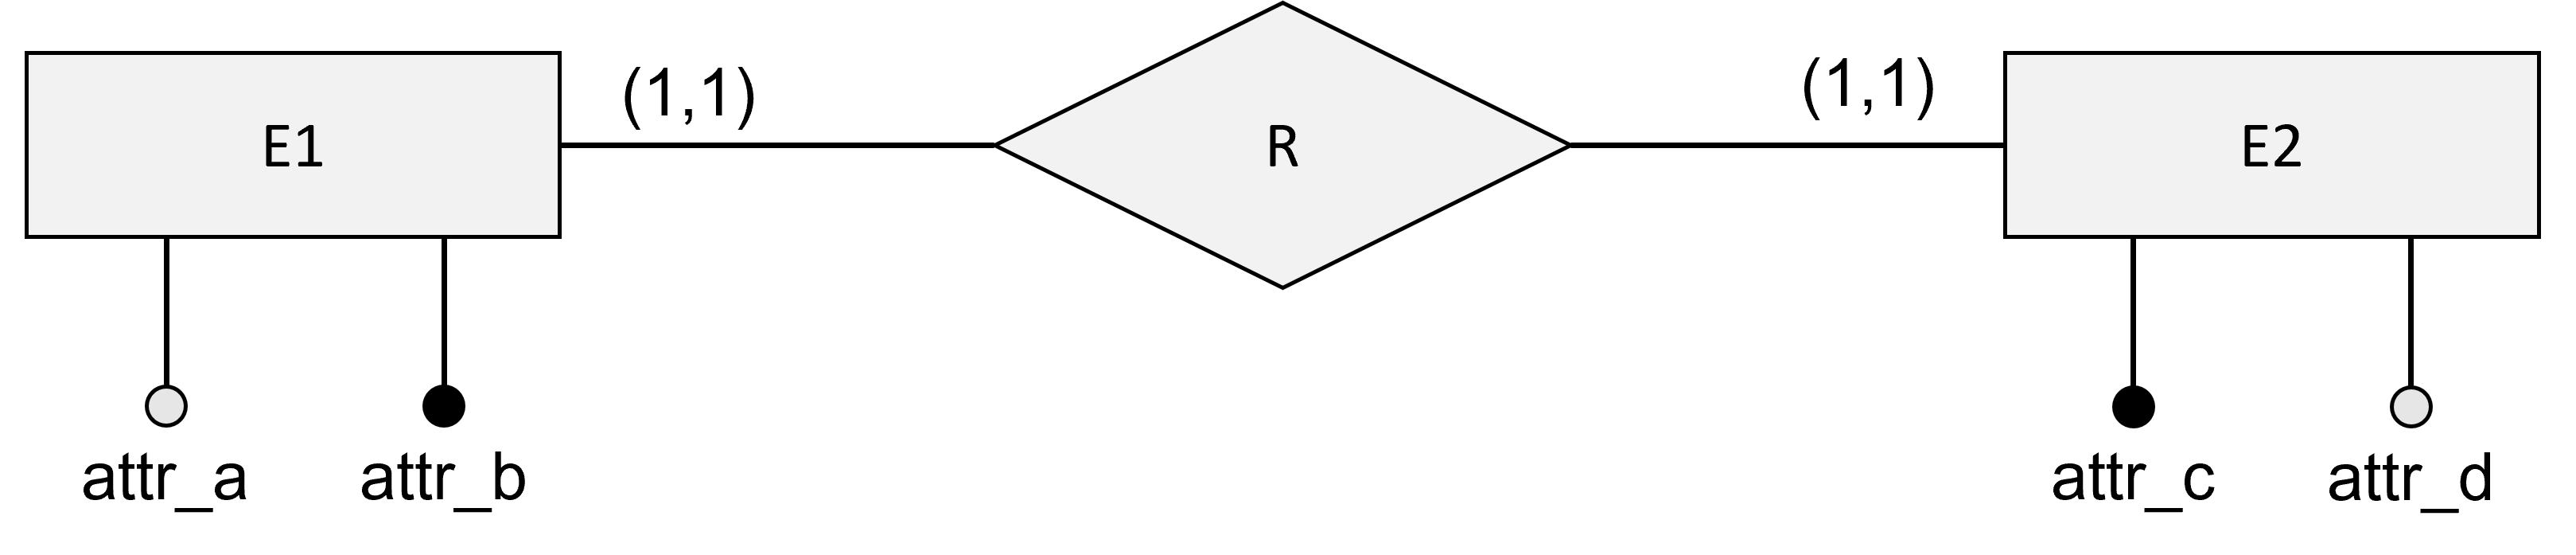
\includegraphics[width=0.65\textwidth, trim=0 0 0 0, clip]{t4/images/case1.png}
	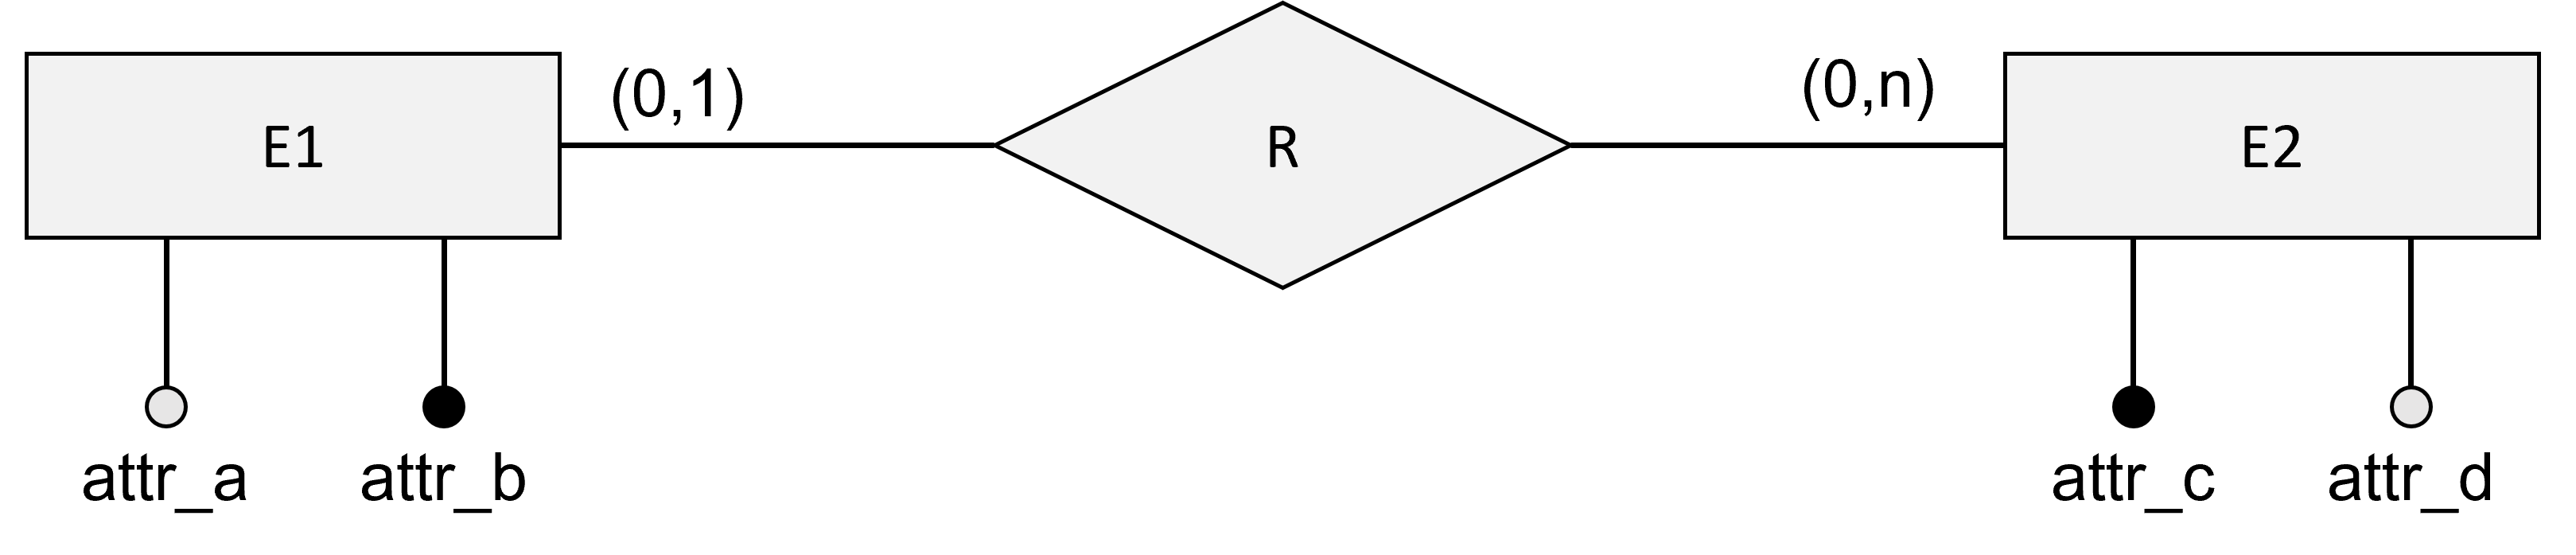
\includegraphics[width=0.65\textwidth, trim=0 0 0 0, clip]{t4/images/case2.png}
	\includegraphics[width=0.65\textwidth, trim=0 0 0 0, clip]{t4/images/case3.png}
	\includegraphics[width=0.65\textwidth, trim=0 0 0 0, clip]{t4/images/case4.png}
\end{figure}
\end{frame}

\begin{frame}[fragile]{Extra Practice (Case 1)}
\begin{figure}
	\includegraphics[width=0.65\textwidth, trim=0 0 0 0, clip]{t4/images/case1.png}
\end{figure}

\begin{columns}
\column{0.5\textwidth}
\begin{figure}
	\centering
	E1 as \textbf{political\_party},\\E2 as \textbf{secretary\_general},\\R as \textbf{led\_by}\vspace{10pt}
	\scriptsize
	
\begin{tikzpicture}[ele/.style={fill=black,minimum size=1pt,circle}, node distance=5pt]
		\node[ele,label=left:People's Action] (a1) {};    
		\node[ele,label=left:Workers (S'pore)] (a2) [below=of a1] {};    
		\node[ele,label=left:Progress Singapore] (a3) [below=of a2] {};
		\node[ele,label=left:Reform (S'pore)] (a4) [below=of a3]  {};
		
		\node[ele,,label=right:Lee Hsien Loong] (b1) [right=of a1,xshift=15pt] {};
		\node[ele,,label=right:Francis Yuen] (b2) [below=of b1] {};
		\node[ele,,label=right:Pritam Singh] (b3) [below=of b2] {};
		\node[ele,,label=right:Kenneth Jeyaretnam] (b4) [below=of b3] {};
		
		%\node[draw,fit= (a1) (a2) (a3) (a4),minimum width=2cm] {} ;
		%\node[draw,fit= (b1) (b2) (b3) (b4),minimum width=2cm] {} ;  
		\draw[-,thick,shorten <=2pt,shorten >=2pt] (a1) -- (b1);
		\draw[-,thick,shorten <=2pt,shorten >=2] (a2) -- (b3);
		\draw[-,thick,shorten <=2pt,shorten >=2] (a3) -- (b2);
		\draw[-,thick,shorten <=2pt,shorten >=2] (a4) -- (b4);
	\end{tikzpicture}
\end{figure}

\column{0.01\textwidth}
\column{0.47\textwidth}
\underline{\textbf{Table E1}}: \\\faIcon{key} name,\\ secretary\_general \\\vspace{5pt}
\textit{or \underline{alternatively}, we define}\\\vspace{5pt}
\underline{\textbf{Table E2}}:\\\faIcon{key} name\\ leading\_party,
\end{columns}
\end{frame}

\begin{frame}[fragile]{Extra Practice (Case 2)}
	\begin{figure}
		\includegraphics[width=0.58\textwidth, trim=0 0 0 0, clip]{t4/images/case2.png}
	\end{figure}
	
	\begin{columns}
		\column{0.52\textwidth}
		\begin{figure}
			\centering
			E1 as \textbf{parliament\_member},\\E2 as \textbf{political\_party},\\R as \textbf{belongs\_to}\vspace{10pt}
			\scriptsize
			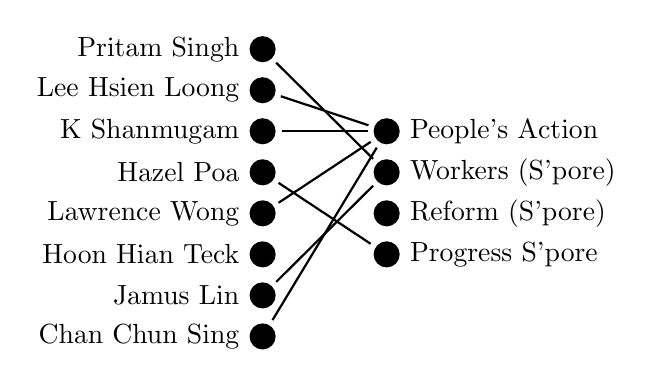
\begin{tikzpicture}[ele/.style={fill=black,minimum size=1pt,circle}, node distance=5pt]
				\node[ele,label=left:Pritam Singh] (a1) {};    
				\node[ele,label=left:Lee Hsien Loong] (a2) [below=of a1] {};    
				\node[ele,label=left:K Shanmugam] (a3) [below=of a2] {};
				\node[ele,label=left:Hazel Poa] (a4) [below=of a3]  {};
				\node[ele,label=left:Lawrence Wong] (a5) [below=of a4]  {};
				\node[ele,label=left:Hoon Hian Teck] (a6) [below=of a5]  {};
				\node[ele,label=left:Jamus Lin] (a7) [below=of a6]  {};
				\node[ele,label=left:Chan Chun Sing] (a8) [below=of a7]  {};
				
				\node[ele,,label=right:People's Action] (b1) [right=of a3,xshift=30pt] {};
				\node[ele,,label=right:Workers (S'pore)] (b2) [below=of b1] {};
				\node[ele,,label=right:Reform (S'pore)] (b3) [below=of b2] {};
				\node[ele,,label=right:Progress S'pore] (b4) [below=of b3] {};
				
				%\node[draw,fit= (a1) (a2) (a3) (a4),minimum width=2cm] {} ;
				%\node[draw,fit= (b1) (b2) (b3) (b4),minimum width=2cm] {} ;  
				\draw[-,thick,shorten <=2pt,shorten >=2pt] (a1) -- (b2);  
				\draw[-,thick,shorten <=2pt,shorten >=2pt] (a7) -- (b2);
				\draw[-,thick,shorten <=2pt,shorten >=2] (a2) -- (b1);
				\draw[-,thick,shorten <=2pt,shorten >=2] (a3) -- (b1);
				\draw[-,thick,shorten <=2pt,shorten >=2] (a5) -- (b1);
				\draw[-,thick,shorten <=2pt,shorten >=2] (a8) -- (b1);
				\draw[-,thick,shorten <=2pt,shorten >=2] (a4) -- (b4);
			\end{tikzpicture}
		\end{figure}
		
		\column{0.48\textwidth}
		\underline{\textbf{Table E1}}: \\\faIcon{key} name \\\vspace{5pt}
		\underline{\textbf{Table E2}}: \\\faIcon{key} name \\\vspace{5pt}
		\underline{\textbf{Table R}}: \\\faIcon{key}~\faIcon{arrow-right} member\_name (E1.name), \\
		\faIcon{arrow-right} affiliation\_party (E2.name)
		\vspace{5pt}
	\end{columns}
\end{frame}


\begin{frame}[fragile]{Extra Practice (Case 3)}
	\begin{figure}
		\includegraphics[width=0.65\textwidth, trim=0 0 0 0, clip]{t4/images/case3.png}
	\end{figure}
	
	\begin{columns}
		\column{0.5\textwidth}
		\begin{figure}
			\centering
			E1 as \textbf{government},\\E2 as \textbf{parliament\_member},\\R as \textbf{head}\vspace{10pt}
			\scriptsize
			
\begin{tikzpicture}[ele/.style={fill=black,minimum size=1pt,circle}, node distance=5pt] 
				\node[ele,label=left:Prime Minister Office] (a1) {};    
				\node[ele,label=left:Ministry of Finance] (a2) [below=of a1] {};    
				\node[ele,label=left:Ministry of Law] (a3) [below=of a2] {};
				\node[ele,label=left:Ministry of Home Affairs] (a4) [below=of a3]  {};
				
				\node[ele,label=right:Pritam Singh] (b1) [right=of a1, above=of a1,xshift=25pt] {};
				\node[ele,,label=right:K Shanmugam] (b2) [below=of b1] {};
				\node[ele,,label=right:Lawrence Wong] (b3) [below=of b2] {};
				\node[ele,,label=right:Jamus Lim] (b4) [below=of b3] {};
				\node[ele,,label=right:Lee Hsien Loong] (b5) [below=of b4] {};
				\node[ele,,label=right:Patrick Tay] (b6) [below=of b5] {};
				
				%\node[draw,fit= (a1) (a2) (a3) (a4),minimum width=2cm] {} ;
				%\node[draw,fit= (b1) (b2) (b3) (b4),minimum width=2cm] {} ;  
				\draw[-,thick,shorten <=1pt,shorten >=1pt] (a1) -- (b5);
				\draw[-,thick,shorten <=1pt,shorten >=1] (a2) -- (b3);
				\draw[-,thick,shorten <=1pt,shorten >=1] (a3) -- (b2);
				\draw[-,thick,shorten <=1pt,shorten >=1] (a4) -- (b2);
			\end{tikzpicture}
		\end{figure}
		
		\column{0.42\textwidth}
		
		\underline{\textbf{Table E1}}: \\\faIcon{key} government\_name\\ \faIcon{arrow-right} name (E2.name) \\\vspace{5pt}
		\underline{\textbf{Table E2}}: \\\faIcon{key} name
	\end{columns}
\end{frame}


\begin{frame}[fragile]{Extra Practice (Case 4)}
	\begin{figure}
		\includegraphics[width=0.65\textwidth, trim=0 0 0 0, clip]{t4/images/case4.png}
	\end{figure}
	
	\begin{columns}
		\column{0.5\textwidth}
		\begin{figure}
			\centering
			E1 as \textbf{party},\\E2 as \textbf{country},\\R as \textbf{belongs\_to}\vspace{10pt}
			\scriptsize
			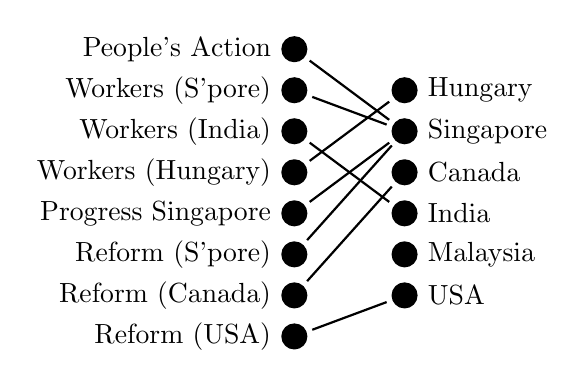
\begin{tikzpicture}[ele/.style={fill=black,minimum size=1pt,circle}, node distance=5pt]
				\node[ele,label=left:People's Action] (a1) {};    
				\node[ele,label=left:Workers (S'pore)] (a2) [below=of a1] {}; 
				\node[ele,label=left:Workers (India)] (a3) [below=of a2] {};
				\node[ele,label=left:Workers (Hungary)] (a4) [below=of a3] {};     
				\node[ele,label=left:Progress Singapore] (a5) [below=of a4] {};
				\node[ele,label=left:Reform (S'pore)] (a6) [below=of a5]  {};
				\node[ele,label=left:Reform (Canada)] (a7) [below=of a6]  {};
				\node[ele,label=left:Reform (USA)] (a8) [below=of a7]  {};
				
				\node[ele,,label=right:Hungary] (b1) [right=of a2,xshift=25pt] {};
				\node[ele,,label=right:Singapore] (b2) [below=of b1] {};
				\node[ele,,label=right:Canada] (b3) [below=of b2] {};
				\node[ele,,label=right:India] (b4) [below=of b3] {};
				\node[ele,,label=right:Malaysia] (b5) [below=of b4] {};
				\node[ele,,label=right:USA] (b6) [below=of b5] {};
				
				%\node[draw,fit= (a1) (a2) (a3) (a4),minimum width=2cm] {} ;
				%\node[draw,fit= (b1) (b2) (b3) (b4),minimum width=2cm] {} ;  
				\draw[-,thick,shorten <=2pt,shorten >=2pt] (a1) -- (b2);
				\draw[-,thick,shorten <=2pt,shorten >=2] (a2) -- (b2);
				\draw[-,thick,shorten <=2pt,shorten >=2] (a5) -- (b2);
				\draw[-,thick,shorten <=2pt,shorten >=2] (a6) -- (b2);
				\draw[-,thick,shorten <=2pt,shorten >=2] (a3) -- (b4);
				\draw[-,thick,shorten <=2pt,shorten >=2] (a4) -- (b1);
				\draw[-,thick,shorten <=2pt,shorten >=2] (a7) -- (b3);
				\draw[-,thick,shorten <=2pt,shorten >=2] (a8) -- (b6);
			\end{tikzpicture}
		\end{figure}
		
		\column{0.02\textwidth}
		\column{0.45\textwidth}
	
		\underline{\textbf{Table E1}}: \\\faIcon{key} party\_name\\ \faIcon{key}~\faIcon{arrow-right} country (E2.name) \\\vspace{5pt}
		\underline{\textbf{Table E2}}: \\\faIcon{key} name
	\end{columns}
\end{frame}
	
\begin{frame}{}
	\centering  
	For any further question, please feel free to email me:\vspace{10pt}
	
	huasong.meng@u.nus.edu \vspace{20pt}
	
	\begin{tcolorbox}
		\begin{center}
			\textcolor{red}{Cases in the extra practice are contributed by our students.\\\vspace{5pt}Copyright 2022 Mark H. Meng. All rights reserved.}
		\end{center}
	\end{tcolorbox}
\end{frame}


\title{BT5110 Data Management and Warehousing}

\subtitle{Tutorial 5: Normalisation\\ \textbf{(Extra Practice)}}

\author{Mark Meng Huasong}

\institute[National University of Singapore] % (optional, but mostly needed)
{
	School of Computing\\
	National University of Singapore
}

\titlegraphic{
	\includegraphics[width=2cm]{nus-logo}
}

\date{4 - 8 Oct, 2021}

\begin{frame}
	\titlepage
	\begin{tcolorbox}
		\begin{center}
			{\scriptsize \textcolor{red}{All the materials within presentation slides are protected by copyrights.\\
					It is forbidden by NUS to upload these materials to the Internet.}}
		\end{center}
	\end{tcolorbox}
\end{frame}

\begin{frame}
	\begin{itemize}
		\item Extra Case No.1 - Warehouse management system
		\item Extra Case No.2 - University transcript issuing system
		\item Extra Case No.3 (Abstract) - \textcolor{red}{\textit{Non dependency preserving decomposition}}
		\item Extra Case No.4 (Abstract) - \textcolor{red}{\textit{Candidate keys with different sizes}}
		\item In-class Case No.1 (Abstract) 
		\item In-class Case No.2 (Abstract) - \textcolor{red}{\textit{Trick wanted for finding candidate key(s)}}
		
	\end{itemize}
\end{frame}

\begin{frame}[fragile]{\boss{Extra} - Case 1}
	We are designing a warehouse management system for a lot of warehouses. Each warehouse ($W$) has one manager ($M$), and each manager only manage one warehouse. There could be many products ($P$) in per warehouse. For each product we also record its stock number ($S$).\\\vspace{10pt}
	\textbf{Questions}:\\
	(1) Find \textbf{candidate key(s)} and \textbf{prime attribute(s)} from attribute closures $\Sigma^{+}$.\\
	(2) Compute the \textbf{compact minimal cover} of $R$ with all FDs $\Sigma$.\\
	(3) Determine if it is \textbf{2NF}? If yes, is it \textbf{3NF}? If yes, is it \textbf{BCNF}?\\
	(4) If it is not 3NF, \textbf{synthesis} the relations to make it 3NF.\\
	(5) If it is not BCNF, \textbf{decomposite} the relations to make it BCNF and verify the \textbf{dependency preservation}. 
\end{frame}

\begin{frame}[fragile]{\boss{Extra} - Case 1 (Solution)}
	\textbf{W}: warehouse; \textbf{M}: manager;
	\textbf{P}: product; \textbf{S}: stock.\\\vspace{5pt}
	$R = \{W, M, P, S\}$\\
	$\Sigma = \{\{W\} \rightarrow \{M\}, \{M\} \rightarrow \{W\},
	\{W, P\} \rightarrow \{S\}\}$.\\\vspace{15pt}
	\begin{figure}
		\includegraphics[width=0.2\textwidth, trim=0 0 0 0, clip]{t5/images/case1.png}
	\end{figure}\vspace{-5pt}
\end{frame}

\begin{frame}[fragile]{\boss{Extra} - Case 1 (Solution)}
	$R = \{W, M, P, S\}$\\
	$\Sigma = \{\{W\} \rightarrow \{M\}, \{M\} \rightarrow \{W\},
	\{W, P\} \rightarrow \{S\}\}$.\\\vspace{5pt}
	
	\textbf{Solution}:\\
	(1) The attribute closure of $R$ is:
	\begin{align*} 
		\Sigma^{+} = \{&\{W\}^{+} \rightarrow \{W, M\},\\
		&\{M\}^{+} \rightarrow \{W, M\},\\
		&\{P\}^{+} \rightarrow \{P\},\\
		&\{S\}^{+} \rightarrow \{S\},\\
		&\{{M,W}\}^{+} \rightarrow \{W, M\},\\
		&\{{M,P}\}^{+} \rightarrow \{W, M, P, S\},\\
		&\{{M,S}\}^{+} \rightarrow \{W, M, S\},\\
		&\{{W,P}\}^{+} \rightarrow \{W, M, P, S\},\\
		&\{{W,S}\}^{+} \rightarrow \{W, M, S\},...\}.
	\end{align*} 
	
	Now we find candidate keys: $\{W, P\}$ and $\{M, P\}$.\\
	Prime attributes: $W, M, P$
\end{frame}

\begin{frame}[fragile]{\boss{Extra} - Case 1 (Solution)}
	(2) The compact minimal cover is:\\\vspace{5pt}
	
	$\{W\} \rightarrow \{M\},$\\
	$\{M\}  \rightarrow \{W\},$\\
	$\{W, P\} \rightarrow \{S\}.$\\\vspace{5pt}
	
	(3)  Yes it is 2NF, 3NF, but not BCNF (e.g., $\{W\} \rightarrow \{M\}$, where $\{W\}$ is not a superkey).\\\vspace{5pt}
	
	(4) Omitted as it is 3NF. \\\vspace{5pt}
	
	(5) Decomposition at $\{W\} \rightarrow \{M\}$:\\\vspace{5pt}
	
	$R_1 = (\underline{W}, \underline{M}),$\\
	$R_2 = (\underline{W}, \underline{P}, S).$\\\vspace{5pt}
	
	It is (luckily) dependency preserving.
	
\end{frame}

\begin{frame}[fragile]{\boss{Extra} - Case 2}
	We are designing a transcript issuing system for our university. 
	Each student is identified by its matric number/student ID, written as $S$.
	We are going to record a grade ($G$) for each student ($S$) and each module ($M$).
	We also record students' names ($N$) and their faculty ($F$). In case any verification is needed, we also save the dean's name for each department ($D$) so that people can contact him/her.\\\vspace{10pt}
	\textbf{Questions}:\\
	(1) Find \textbf{candidate key(s)} and \textbf{prime attribute(s)} from attribute closures $\Sigma^{+}$.\\
	(2) Compute the \textbf{compact minimal cover} of $R$ with all FDs $\Sigma$.\\
	(3) Determine if it is \textbf{2NF}? If yes, is it \textbf{3NF}? If yes, is it \textbf{BCNF}?\\
	(4) If it is not 3NF, \textbf{synthesis} the relations to make it 3NF.\\
	(5) If it is not BCNF, \textbf{decomposite} the relations to make it BCNF and verify the \textbf{dependency preservation}. 
\end{frame}

\begin{frame}[fragile]{\boss{Extra} - Case 2 (Solution)}
	\textbf{S}: student ID; \textbf{M}: module; \textbf{N}: name;
	\textbf{F}: faculty; \textbf{G}: grade; \textbf{D}: dean\\\vspace{5pt}
	$R = \{S, M, G, N, F, D\}$\\
	$\Sigma = \{\{S, M\} \rightarrow \{G\}, 
	\{S\} \rightarrow \{N, F\},
	\{F\} \rightarrow \{D\}\}$.\\\vspace{15pt}
	\begin{figure}
		\includegraphics[width=0.4\textwidth, trim=0 0 0 0, clip]{t5/images/case2.png}
	\end{figure}\vspace{-5pt}
\end{frame}

\begin{frame}[fragile]{\boss{Extra} - Case 2 (Solution)}
	$R = \{S, M, G, N, F, D\}$\\
	$\Sigma = \{\{S, M\} \rightarrow \{G\}, 
	\{S\} \rightarrow \{N, F\},
	\{F\} \rightarrow \{D\}\}$.\\\vspace{5pt}
	
	\textbf{Solution}:\\
	(1) The attribute closure of $R$ is:
	\begin{align*} 
		\Sigma^{+} = \{&\{S\}^{+} \rightarrow \{S, N, F, D\},\\
		&\{M\}^{+} \rightarrow \{M\},\\
		&\{G\}^{+} \rightarrow \{G\},\\
		&\{N\}^{+} \rightarrow \{N\},\\
		&\{F\}^{+} \rightarrow \{F, D\},\\
		&\{D\}^{+} \rightarrow \{D\},\\
		&\{{S, M}\}^{+} \rightarrow \{S, M, N, F, D, G\},\\
		&\{{S, G}\}^{+} \rightarrow \{S, G, N, F, D\}, ...
	\end{align*} 
	
	Now we find candidate keys: $\{S, M\}$.\\
	Prime attributes: $S, M$
\end{frame}

\begin{frame}[fragile]{\boss{Extra} - Case 2 (Solution)}
	(2) The compact minimal cover is:\\\vspace{5pt}
	
	$\{S, M\} \rightarrow \{G\},$\\
	$\{S\}  \rightarrow \{N, F\},$\\
	$\{F\} \rightarrow \{D\}.$\\\vspace{5pt}
	
	(3)  No it is not 2NF (e.g., $\{S\}\rightarrow\{N, F\}$, \{N, F\} are not prime attributes and $S$ is a subset of candidate key). Therefore it is not 3NF, and not BCNF, too.\\\vspace{5pt}
	
	(4) Synthesis result has 3 relations and is (luckily) BCNF: \\\vspace{5pt}
	
	$R_1 = (\underline{S}, \underline{M}, G),$\\
	$R_2 = (\underline{S}, N, F),$\\
	$R_3 = (\underline{F}, D).$\\\vspace{5pt}
	
\end{frame}

\begin{frame}[fragile]{\boss{Extra} - Case 2 (Solution)}
	(5) Decomposition at $\{F\} \rightarrow \{D\}$:\\\vspace{5pt}
	
	$R_1 = (\underline{F}, D),$\\
	$R_2 = (\underline{S}, \underline{M}, G, N, F).$\\\vspace{5pt}
	
	However, $R_2$ needs to be further decomposed, at $\{S\} \rightarrow \{N\}$:\\\vspace{5pt}
	
	$R_{2.1} = (\underline{S}, N, F).$\\
	$R_{2.2} = (\underline{S}, \underline{M}, G).$\\\vspace{5pt}
	
	As the result, the BCNF decomposition is (luckily) dependency preserving and is given below:\\\vspace{5pt}
	
	$R_1 = (\underline{F}, D),$\\
	$R_{2.1} = (\underline{S}, N, F).$\\
	$R_{2.2} = (\underline{S}, \underline{M}, G).$\\\vspace{5pt}
	
	\textit{(In fact this decomposition result is same with the synthesis one)}
\end{frame}

\begin{frame}[fragile]{\boss{Extra} - Case 3}
	This time we deal with abstract relations with functional dependencies shown as in the figure below:\\\vspace{-5pt}
	
	\begin{figure}
		\includegraphics[width=0.4\textwidth, trim=0 0 0 0, clip]{t5/images/case3.png}
	\end{figure}\vspace{-10pt}
	
	\textbf{Questions}:\\
	(1) Find \textbf{candidate key(s)} and \textbf{prime attribute(s)} from attribute closures $\Sigma^{+}$.\\
	(2) Compute the \textbf{compact minimal cover} of $R$ with all FDs $\Sigma$.\\
	(3) Determine if it is \textbf{2NF}? If yes, is it \textbf{3NF}? If yes, is it \textbf{BCNF}?\\
	(4) If it is not 3NF, \textbf{synthesis} the relations to make it 3NF.\\
	(5) If it is not BCNF, \textbf{decomposite} the relations to make it BCNF and verify the \textbf{dependency preservation}. 
\end{frame}


\begin{frame}[fragile]{\boss{Extra} - Case 3 (Solution)}
	
	\textbf{Solution}:\\
	(1) The attribute closure of $R = \{A, B, C, D\}$ is:\\\vspace{5pt}
	\begin{scriptsize}
		\begin{align*} 
			\Sigma^{+} = \{&\{A\}^{+} \rightarrow \{A\},\\
			&\{B\}^{+} \rightarrow \{B\},\\
			&\{C\}^{+} \rightarrow \{A, C, D\},\\
			&\{D\}^{+} \rightarrow \{A, D\},\\
			&\{A, B\}^{+} \rightarrow \{A, B, C, D\},\\
			&\{A, C\}^{+} \rightarrow \{A, C, D\},\\
			&\{A, D\}^{+} \rightarrow \{A, D\},\\
			&\{B, C\}^{+} \rightarrow \{A, B, C, D\}\\
			&\{B, D\}^{+} \rightarrow \{A, B, C, D\}, ...
		\end{align*}
	\end{scriptsize}
	
	Now we find candidate keys: $\{A, B\}$ or $\{B, C\}$ or $\{B, D\}$.\\
	Prime attributes: $A, B, C, D$ (There is no non-prime attribute for this case)
\end{frame}

\begin{frame}[fragile]{\boss{Extra} - Case 3 (Solution)}
	(2) The compact minimal cover is:\\\vspace{5pt}
	
	$\{A, B\} \rightarrow \{C\}$\\
	$\{C\} \rightarrow \{D\}$\\
	$\{D\} \rightarrow \{A\}$.\\\vspace{5pt}
	
	(3) Yes it is 2NF and 3NF (because all attributes are prime attributes). However, it is not BCNF (e.g., $\{C\} \rightarrow \{D\}$ and $\{D\} \rightarrow \{A\}$).\\\vspace{5pt}
	
	(4) Omitted as it is 3NF. \\\vspace{5pt}
	
\end{frame}

\begin{frame}[fragile]{\boss{Extra} - Case 3 (Solution)}
	(5) Decomposition at $\{C\} \rightarrow \{D\}$:\\\vspace{5pt}
	
	$R_1 = (A, \underline{C}, D),$\\
	$R_2 = (\underline{B}, \underline{C}).$\\\vspace{5pt}
	
	In this way both relations are BCNF, but we lose a dependency $\{A, B\} \rightarrow \{C\}$.\\\vspace{5pt}
	
	\textcolor{red}{How about we change the entry point of decomposition?}\\\vspace{5pt}
	
	Decomposition at $\{D\} \rightarrow \{A\}$:\\\vspace{5pt}
	
	$R_1 = (A, \underline{D}),$\\
	$R_2 = (B, \underline{C}, D).$\\\vspace{5pt}
	
	In this way both relations are BCNF, but we (still) lose that dependency $\{A, B\} \rightarrow \{C\}$.
\end{frame}

\begin{frame}[fragile]{\boss{Extra} - Case 4}
	Another abstract relations with functional dependencies shown as in the figure below:\\\vspace{-5pt}
	
	\begin{figure}
		\includegraphics[width=0.25\textwidth, trim=0 0 0 0, clip]{t5/images/case4.png}
	\end{figure}\vspace{-5pt}
	
	\textbf{Questions}:\\
	(1) Find \textbf{candidate key(s)} and \textbf{prime attribute(s)} from attribute closures $\Sigma^{+}$.\\
	(2) Compute the \textbf{compact minimal cover} of $R$ with all FDs $\Sigma$.\\
	(3) Determine if it is \textbf{2NF}? If yes, is it \textbf{3NF}? If yes, is it \textbf{BCNF}?\\
	(4) If it is not 3NF, \textbf{synthesis} the relations to make it 3NF.\\
	(5) If it is not BCNF, \textbf{decomposite} the relations to make it BCNF and verify the \textbf{dependency preservation}. 
\end{frame}


\begin{frame}[fragile]{\boss{Extra} - Case 4 (Solution)}
	
	\textbf{Solution}:\\
	(1) The attribute closure of $R = \{A, B, C, D\}$ is:\\\vspace{5pt}
	\begin{scriptsize}
		\begin{align*} 
			\Sigma^{+} = \{&\{A\}^{+} \rightarrow \{A, B, C, D\},\\
			&\{B\}^{+} \rightarrow \{B, D\},\\
			&\{C\}^{+} \rightarrow \{C\},\\
			&\{D\}^{+} \rightarrow \{D\},\\
			&\{A, B\}^{+} \rightarrow \{A, B, C, D\},\\
			&\{A, C\}^{+} \rightarrow \{A, B, C, D\} (trivial),\\
			&\{A, D\}^{+} \rightarrow \{A, B, C, D\} (trivial),\\
			&\{B, C\}^{+} \rightarrow \{A, B, C, D\}\\
			&\{B, D\}^{+} \rightarrow \{B, D\}, ...
		\end{align*}
	\end{scriptsize}
	
	Now we find candidate keys: $\{A\}$ or $\{B, C\}$.\\
	Prime attributes: $A, B, C$.
\end{frame}

\begin{frame}[fragile]{\boss{Extra} - Case 4 (Solution)}
	(2) The compact minimal cover is:\\\vspace{5pt}
	
	$\{A\} \rightarrow \{B, C, D\}$\\
	$\{B\} \rightarrow \{D\}$\\
	$\{B, C\} \rightarrow \{A\}$.\\\vspace{5pt}
	
	(3) No it is not 2NF (e.g., $\{B\} \rightarrow \{D\}$, where $D$ is a non-prime attribute but $B$ is a subset of candidate key). Therefore, it is not 3NF and not BCNF, too.\\\vspace{5pt}
	
	(4) Synthesis result has 2 relations and each one is (luckily) BCNF: \\\vspace{5pt}
	
	$R_1 = (\underline{A}, \underline{B, C}, D),$\\\vspace{2pt}
	$R_2 = (\underline{B}, D),$\\\vspace{1pt}
	$\cancel{R_3 = (\underline{B, C}, \underline{A})}.$ (duplicate with $R_1$)\\\vspace{5pt}
	
\end{frame}

\begin{frame}[fragile]{\boss{Extra} - Case 4 (Solution)}
	(5) Decomposition at $\{B\} \rightarrow \{D\}$:\\\vspace{5pt}
	
	$R_1 = (\underline{B}, D),$\\
	$R_2 = (\underline{A}, \underline{B, C}).$\\\vspace{5pt}
	
	In this way both relations are BCNF, but we lose a dependency $\{A\} \rightarrow \{D\}$.\\\vspace{5pt}
	
\end{frame}

\begin{frame}[fragile]{\boss{Extra} - In-class Case 1}
	Given a relation $R=\{A, B, C\}$ with functional dependency set:\\ 
	$\Sigma=\{\{A\} \rightarrow \{B\},\{B\} \rightarrow \{C\}, \{A, B\} \rightarrow \{C\},\{B, C\} \rightarrow \{A\}\}.$\\\vspace{10pt}
	\textbf{Questions}:\\
	(1) Find \textbf{candidate key(s)} and \textbf{prime attribute(s)} from attribute closures $\Sigma^{+}$.\\
	(2) Compute the \textbf{compact minimal cover} of $R$ with all FDs $\Sigma$.\\
	(3) Determine if it is \textbf{2NF}? If yes, is it \textbf{3NF}? If yes, is it \textbf{BCNF}?\\
	(4) If it is not 3NF, \textbf{synthesis} the relations to make it 3NF.\\
	(5) If it is not BCNF, \textbf{decomposite} the relations to make it BCNF and verify the \textbf{dependency preservation}. 
\end{frame}

\begin{frame}[fragile]{\boss{Extra} - In-class Case 1 (Solution)}
	$R=\{A, B, C\}$\\ 
	$\Sigma=\{\{A\} \rightarrow \{B\},\{B\} \rightarrow \{C\}, \{A, B\} \rightarrow \{C\},\{B, C\} \rightarrow \{A\}\}.$\\\vspace{5pt}
	
	\textbf{Solution}:\\
	(1) The attribute closure of $R$ is:
	\begin{align*} 
		\Sigma^{+} = \{&\{A\}^{+} \rightarrow \{A,B,C\},\\
		&\{B\}^{+} \rightarrow \{A,B,C\},\\
		&\{C\}^{+} \rightarrow \{C\},\\
		&\{A,B\}^{+} \rightarrow \{A,B,C\},\\
		&\{A,C\}^{+} \rightarrow \{A,B,C\},\\
		&\{B,C\}^{+} \rightarrow \{A,B,C\},\\
		&\{A,B,C\}^{+} \rightarrow \{A,B,C\}\}.
	\end{align*} 
	
	Now we find candidate keys: $\{A\}$ and $\{B\}$.\\
	Prime attributes: $A, B$
\end{frame}

\begin{frame}[fragile]{\boss{Extra} - In-class Case 1 (Solution)}
	$\Sigma=\{\{A\} \rightarrow \{B\},\{B\} \rightarrow \{C\}, \{A, B\} \rightarrow \{C\},\{B, C\} \rightarrow \{A\}\}.$\\\vspace{25pt}
	
	(2) The minimal cover is:\\\vspace{5pt}
	
	$\{A\} \rightarrow \{B\},$\\
	$\{B\}  \rightarrow \{C\},$\\
	$\{B,C\} \rightarrow \{A\}.$\\\vspace{5pt}
	
	This is the compact minimal cover, too.\\\vspace{5pt}
	
	(3)  Yes it is 2NF, 3NF, and BCNF, too.\\\vspace{5pt}
	
	(4) Omitted as it is 3NF. \\\vspace{5pt}
	
	(5) Omitted as it is BCNF. \\\vspace{5pt}
	
\end{frame}

\begin{frame}[fragile]{\boss{Extra} - In-class Case 2}
	Given a relation $R=\{A, B, C, D, E\}$ with functional dependency set:\\ 
	$\Sigma=\{\{C,D\} \rightarrow \{E\},\{A,B\} \rightarrow \{B\}, \{A,C,D\} \rightarrow \{E\},\{A\} \rightarrow \{E\},\{D,E\} \rightarrow \{B,C\},\{A\} \rightarrow \{A\}\}.$\\\vspace{10pt}
	\textbf{Questions}:\\
	(1) Find \textbf{candidate key(s)} and \textbf{prime attribute(s)} from attribute closures $\Sigma^{+}$.\\
	(2) Compute the \textbf{compact minimal cover} of $R$ with all FDs $\Sigma$.\\
	(3) Determine if it is \textbf{2NF}? If yes, is it \textbf{3NF}? If yes, is it \textbf{BCNF}?\\
	(4) If it is not 3NF, \textbf{synthesis} the relations to make it 3NF.\\
	(5) If it is not BCNF, \textbf{decomposite} the relations to make it BCNF and verify the \textbf{dependency preservation}. 
\end{frame}

\begin{frame}[fragile]{\boss{Extra} - In-class Case 2 (Solution)}
	$\Sigma=\{\{C,D\} \rightarrow \{E\},\{A,B\} \rightarrow \{B\}, \{A,C,D\} \rightarrow \{E\},\{A\} \rightarrow \{E\},\{D,E\} \rightarrow \{B,C\},\{A\} \rightarrow \{A\}\}.$\\\vspace{5pt}
	
	\textbf{Solution}:\\
	(1) The attribute closure of $R$ is:
	\vspace{-10pt}\begin{columns}
	\column{0.35\textwidth}
	\begin{scriptsize}\begin{align*} 
		\Sigma^{+} = \{&\{A\}^{+} \rightarrow \{A,E\},\\
		&\{B\}^{+} \rightarrow \{B\},\\
		&\{C\}^{+} \rightarrow \{C\},\\
		&\{D\}^{+} \rightarrow \{D\},\\
		&\{E\}^{+} \rightarrow \{E\},\\
		&\{A,B\}^{+} \rightarrow \{A,B,E\},\\
		&\{A,C\}^{+} \rightarrow \{A,C,E\},\\
		&\{A,D\}^{+} \rightarrow \{A,D\},\\
		&\{A,E\}^{+} \rightarrow \{A,B,E\}\}\\
		& ...\\
		&\{A,C,D,E\}^{+} \rightarrow \{A,B,C,D,E\}\}\\
		&\{A,B,C,D,E\}^{+} \rightarrow \{A,B,C,D,E\}\}.
	\end{align*}\end{scriptsize} 
	
	\column{0.45\textwidth}
	\textbf{Hint}:\\
	After removing all trivial FDs, we find $A$ and $D$ have never appeared in the right-hand side, which means the candidate key must contains $A$ and $D$. We just need to find the minimal set that implies $\{B,C,E\}$.\\\vspace{10pt}

	Then we can find candidate key: $\{A,C,D,E\}$.\\
	Prime attributes: $A, C, D, E$
	\end{columns}
	
\end{frame}

\begin{frame}[fragile]{\boss{Extra} - In-class Case 2 (Solution)}
	$\Sigma=\{\{C,D\} \rightarrow \{E\},\{A,B\} \rightarrow \{B\}, \{A,C,D\} \rightarrow \{E\},\{A\} \rightarrow \{E\},\{D,E\} \rightarrow \{B,C\},\{A\} \rightarrow \{A\}\}.$\\\vspace{5pt}
	
	(2) The compact minimal cover is:\\\vspace{5pt}
	
	\begin{columns}
	\column{0.35\textwidth}
	$\{C,D\} \rightarrow \{E\},$\\
	$\cancel{\{A,B\} \rightarrow \{B\}}$,\\
	$\cancel{\{A,C,D\} \rightarrow \{E\}}$,\\
	$\{A\}  \rightarrow \{E\},$\\
	$\{D,E\} \rightarrow \{B\}.$\\
	$\{D,E\} \rightarrow \{C\}.$\\
	$\cancel{\{A\} \rightarrow \{A\}}$\\\vspace{5pt}
	\column{0.05\textwidth} $\rightarrow$
	\column{0.45\textwidth}
	So the finalized set is:\\
	$\{C,D\} \rightarrow \{E\},$\\
	$\{A\}  \rightarrow \{E\},$\\
	$\{D,E\} \rightarrow \{B\}.$\\
	$\{D,E\} \rightarrow \{C\}.$\\
	\end{columns}
	
	(3)  No it is not 2NF, not 3NF, and not BCNF, too.\\\vspace{5pt}
	
	$\{D,E\} \rightarrow \{B\}$ violates 2NF.\\
	$\{D,E\} \rightarrow \{B\}$ violates 3NF.\\
	All FDs in minimal cover violate BCNF.
	
\end{frame}


\begin{frame}[fragile]{\boss{Extra} - In-class Case 2 (Solution)}
	(4) Recall the compact minimal cover:\\\vspace{5pt}
	
	$\{C,D\} \rightarrow \{E\},$\\
	$\{A\}  \rightarrow \{E\},$\\
	$\{D,E\} \rightarrow \{B\}.$\\
	$\{D,E\} \rightarrow \{C\}.$\\\vspace{5pt}
	
	Let's do 3NF synthesis:\\ \vspace{5pt}
	\begin{columns}
	\column{0.35\textwidth}
	$R_1 = (\underline{C, D}, E),$\\
	$R_2 = (\underline{A}, E),$\\
	$R_3 = (B, \underline{D, E}).$\\
	$R_4 = (C, \underline{D, E}).$\\
	$R_5 = (\underline{A,C,D,E}).$\\\vspace{5pt}
	\column{0.05\textwidth} $\rightarrow$
	\column{0.35\textwidth}
	So the simplified result is:\\
	$R_1 = (\underline{A, C, D, E}),$\\
	$R_2 = (B, \underline{D, E}),$\\
	
	\end{columns}
	Both relation are BCNF.

\end{frame}

\begin{frame}[fragile]{\boss{Extra} - In-class Case 2 (Solution)}
	(5) Recall the compact minimal cover:\\
	
	$\{C,D\} \rightarrow \{E\},$\\
	$\{A\}  \rightarrow \{E\},$\\
	$\{D,E\} \rightarrow \{B\}.$\\
	$\{D,E\} \rightarrow \{C\}.$\\\vspace{5pt}
	
	Decomposition at $\{C,D\} \rightarrow \{E\}$:\\\vspace{5pt}
		
	$R_1 = (\underline{C,D}, E),$\\
	$R_2 = (\underline{A}, B, \underline{C,D}).$\\\vspace{5pt}
	
	We can find that:\\\vspace{5pt}
	$\Sigma_1 = \{\{C,D\}\rightarrow\{E\}\}$
	$\Sigma_2 = \emptyset$
	
	Both relations are BCNF\\\vspace{5pt}
	However, we lose lots of dependency in this decomposition.
\end{frame}

\begin{frame}{}
	\centering  
	For any further question, please feel free to email me:\vspace{10pt}
	
	huasong.meng@u.nus.edu\\\vspace{3pt}
	
	\begin{tcolorbox}
		\begin{center}
			\textcolor{red}{Copyright 2021 Mark H. Meng. All rights reserved.}
		\end{center}
	\end{tcolorbox}
\end{frame}
%%\begin{comment}
\begin{frame}[fragile]{\boss{Extra Exercise}}
	There are four extra exercises for you to practice what have learned in normalisation lecture. 
	As normalisation is one of the most challenging parts of the fundamental database module, it would be helpful for you to evaluate your understanding of this part. \\
\end{frame}
\end{comment}

\begin{frame}[fragile]{\boss{Extra} - Case 1}
	We are designing a warehouse management system for a lot of warehouses. Each warehouse ($W$) has one manager ($M$), and each manager only manage one warehouse. There could be many products ($P$) in per warehouse. For each product we also record its stock number ($S$).\\\vspace{10pt}
	\textbf{Questions}:\\
	(1) Find \textbf{candidate key(s)} and \textbf{prime attribute(s)} from attribute closures $\Sigma^{+}$.\\
	(2) Compute the \textbf{compact minimal cover} of $R$ with all FDs $\Sigma$.\\
	(3) Determine if it is \textbf{2NF}? If yes, is it \textbf{3NF}? If yes, is it \textbf{BCNF}?\\
	(4) If it is not 3NF, \textbf{synthesis} the relations to make it 3NF.\\
	(5) If it is not BCNF, \textbf{decomposite} the relations to make it BCNF and verify the \textbf{dependency preservation}. 
\end{frame}

\begin{frame}[fragile]{\boss{Extra} - Case 2}
	We are designing a transcript issuing system for our university. 
	Each student is identified by its matric number/student ID, written as $S$.
	We are going to record a grade ($G$) for each student ($S$) and each module ($M$).
	We also record students' names ($N$) and their faculty ($F$). In case any verification is needed, we also save the dean's name for each department ($D$) so that people can contact him/her.\\\vspace{10pt}
	\textbf{Questions}:\\
	(1) Find \textbf{candidate key(s)} and \textbf{prime attribute(s)} from attribute closures $\Sigma^{+}$.\\
	(2) Compute the \textbf{compact minimal cover} of $R$ with all FDs $\Sigma$.\\
	(3) Determine if it is \textbf{2NF}? If yes, is it \textbf{3NF}? If yes, is it \textbf{BCNF}?\\
	(4) If it is not 3NF, \textbf{synthesis} the relations to make it 3NF.\\
	(5) If it is not BCNF, \textbf{decomposite} the relations to make it BCNF and verify the \textbf{dependency preservation}. 
\end{frame}

\begin{frame}[fragile]{\boss{Extra} - Case 3}
	This time we deal with abstract relations with functional dependencies shown as in the figure below:\\\vspace{-5pt}
	
	\begin{figure}
		\includegraphics[width=0.4\textwidth, trim=0 0 0 0, clip]{t5/images/case3.png}
	\end{figure}\vspace{-10pt}
	
	\textbf{Questions}:\\
	(1) Find \textbf{candidate key(s)} and \textbf{prime attribute(s)} from attribute closures $\Sigma^{+}$.\\
	(2) Compute the \textbf{compact minimal cover} of $R$ with all FDs $\Sigma$.\\
	(3) Determine if it is \textbf{2NF}? If yes, is it \textbf{3NF}? If yes, is it \textbf{BCNF}?\\
	(4) If it is not 3NF, \textbf{synthesis} the relations to make it 3NF.\\
	(5) If it is not BCNF, \textbf{decomposite} the relations to make it BCNF and verify the \textbf{dependency preservation}. 
\end{frame}

\begin{frame}[fragile]{\boss{Extra} - Case 4}
	Another abstract relations with functional dependencies shown as in the figure below:\\\vspace{-5pt}
	
	\begin{figure}
		\includegraphics[width=0.25\textwidth, trim=0 0 0 0, clip]{t5/images/case4.png}
	\end{figure}\vspace{-5pt}
	
	\textbf{Questions}:\\
	(1) Find \textbf{candidate key(s)} and \textbf{prime attribute(s)} from attribute closures $\Sigma^{+}$.\\
	(2) Compute the \textbf{compact minimal cover} of $R$ with all FDs $\Sigma$.\\
	(3) Determine if it is \textbf{2NF}? If yes, is it \textbf{3NF}? If yes, is it \textbf{BCNF}?\\
	(4) If it is not 3NF, \textbf{synthesis} the relations to make it 3NF.\\
	(5) If it is not BCNF, \textbf{decomposite} the relations to make it BCNF and verify the \textbf{dependency preservation}. 
\end{frame}



\end{document}